\documentclass[11pt, twoside, a4paper]{scrreprt}

%%%%%%%%%%%%%%%%%%%%%%%%%
%% Place packages here %%
%%%%%%%%%%%%%%%%%%%%%%%%%

\usepackage[T1]{fontenc}

% Math
\usepackage{amsmath, amssymb}

% Color
\usepackage{color}
\usepackage[dvipsnames]{xcolor}

% Figure
\usepackage{graphicx}
\usepackage{rotating}
\usepackage{eso-pic}

% Tables
\usepackage{tabularx}
\newcolumntype{L}[1]{>{\hsize=#1\hsize\raggedright\arraybackslash}X}
\newcolumntype{C}[1]{>{\hsize=#1\hsize\centering\arraybackslash}X}
\def\arraystretch{1.5}

% Code
\usepackage{alltt}

% Style options
\PassOptionsToPackage{utf8}{inputenc}
\usepackage{inputenc}

\newcommand{\thesisTitle}{Development of the DAQ System of Triple-GEM Detectors for the CMS Muon Spectrometer Upgrade at LHC}
\newcommand{\thesisName}{Thomas Lenzi}
\newcommand{\thesisSubject}{PhD Thesis}
\newcommand{\thesisDate}{October 2016}
\newcommand{\thesisVersion}{}

\newcommand{\thesisFirstReviewer}{Jane Doe}
\newcommand{\thesisFirstReviewerUniversity}{\protect{Clean Thesis Style University}}
\newcommand{\thesisFirstReviewerDepartment}{Department of Clean Thesis Style}

\newcommand{\thesisSecondReviewer}{John Doe}
\newcommand{\thesisSecondReviewerUniversity}{\protect{Clean Thesis Style University}}
\newcommand{\thesisSecondReviewerDepartment}{Department of Clean Thesis Style}

\newcommand{\thesisFirstSupervisor}{Prof. Gilles De Lentdecker}

\newcommand{\thesisUniversity}{\protect{Université Libre de Bruxelles}}
\newcommand{\thesisUniversityDepartment}{Département de Physique}
\newcommand{\thesisUniversityInstitute}{IIHE - Interuniversity Institute for High Energies}
\newcommand{\thesisUniversityCity}{Brussels}
\newcommand{\thesisUniversityStreetAddress}{Boulevard du Triomphe, 2}
\newcommand{\thesisUniversityPostalCode}{1050}


\usepackage[english]{babel} % babel system, adjust the language of the content
\PassOptionsToPackage{% setup clean thesis style
    figuresep=endash,%
    sansserif=false,%
    hangfigurecaption=false,%
    hangsection=true,%
    hangsubsection=true,%
    colorize=bw,%
    colortheme=bluemagenta,%
    bibsys=bibtex,%
    bibfile=bibliography,%
    bibstyle=numeric,%
    wrapfooter=false,%
}{cleanthesis}
\usepackage{cleanthesis}

\hypersetup{% setup the hyperref-package options
    pdftitle={\thesisTitle},    %   - title (PDF meta)
    pdfsubject={\thesisSubject},%   - subject (PDF meta)
    pdfauthor={\thesisName},    %   - author (PDF meta)
    plainpages=false,           %   -
    colorlinks=false,           %   - colorize links?
    pdfborder={0 0 0},          %   -
    breaklinks=true,            %   - allow line break inside links
    bookmarksnumbered=true,     %
    bookmarksopen=true          %
}


%%%%%%%%%%%
%% Begin %%
%%%%%%%%%%%

\begin{document}

  %%%%%%%%%%%%%%%%%%%%%%%%%%%%%%%%
  %% Front matter of the thesis %%
  %% Title pages, abstract, ... %%
  %%%%%%%%%%%%%%%%%%%%%%%%%%%%%%%%

  \pagenumbering{roman}
  \pagestyle{empty}

  % % Title
  % \begin{titlepage}
  \AddToShipoutPictureBG*{
    \AtPageUpperLeft{\raisebox{-\height}{\includegraphics[width=\paperwidth]{img/0-0-title/logo.jpg}}}
  }
  \tgherosfont
	\centering

  \vspace*{\fill}
	{ \large \thesisSubject } \\[5mm]
	{ \LARGE \color{ctcolortitle} \textbf{\thesisTitle} \\[10mm] }
	{ \Large \thesisName } \\
	\vfill
  % Supervisor
	\begin{minipage}[t]{.27\textwidth}
		\raggedleft
		\textit{Supervisor}
	\end{minipage}
	\hspace*{15pt}
	\begin{minipage}[t]{.65\textwidth}
		\Large \thesisFirstSupervisor
	\end{minipage} \\[30mm]

	\thesisDate \\

\end{titlepage}


% ------------------------------------  --> main title page
\begin{titlepage}
	\tgherosfont
	\centering

	{ \Large \thesisUniversity } \\[4mm]
	\textsf{\thesisUniversityDepartment} \\
	\textsf{\thesisUniversityInstitute} \\

	\vfill
	{ \large \thesisSubject } \\[5mm]
	{ \LARGE \color{ctcolortitle} \textbf{\thesisTitle} \\[10mm] }
	{ \Large \thesisName } \\

	\vfill
  \begin{minipage}[t]{.27\textwidth}
    \raggedleft \hfill
  \end{minipage}
  \hspace*{15pt}
  \begin{minipage}[t]{.65\textwidth}
    { \small Jury members }
  \end{minipage} \\[3mm]
  % Supervisor
	\begin{minipage}[t]{.27\textwidth}
		\raggedleft
		\textit{Supervisor}
	\end{minipage}
	\hspace*{15pt}
	\begin{minipage}[t]{.65\textwidth}
		{ \Large \thesisFirstSupervisor } \\
    { \small \thesisFirstSupervisorUniversity }
	\end{minipage} \\[3mm]
  % Reviewers
	\begin{minipage}[t]{.27\textwidth}
		\raggedleft
		\textit{President}
	\end{minipage}
	\hspace*{15pt}
	\begin{minipage}[t]{.65\textwidth}
		{ \Large \thesisFirstReviewer } \\
	  { \small \thesisFirstReviewerUniversity }
	\end{minipage} \\[3mm]
	\begin{minipage}[t]{.27\textwidth}
		\raggedleft
		\textit{Secretary}
	\end{minipage}
	\hspace*{15pt}
	\begin{minipage}[t]{.65\textwidth}
		{ \Large \thesisSecondReviewer } \\
	  { \small \thesisSecondReviewerUniversity }
	\end{minipage} \\[3mm]
	\begin{minipage}[t]{.27\textwidth}
		\raggedleft
		\textit{Reviewers}
	\end{minipage}
	\hspace*{15pt}
	\begin{minipage}[t]{.65\textwidth}
		{ \Large \thesisThirdReviewer } \\
	  { \small \thesisThirdReviewerUniversity } \\[3mm]
		{ \Large \thesisFourthReviewer } \\
	  { \small \thesisFourthReviewerUniversity } \\[3mm]
		{ \Large \thesisFifthReviewer } \\
	  { \small \thesisFifthReviewerUniversity } \\[3mm]
		{ \Large \thesisSixthReviewer } \\
	  { \small \thesisSixthReviewerUniversity } \\[3mm]
		{ \Large \thesisSeventhReviewer } \\
	  { \small \thesisSeventhReviewerUniversity }
	\end{minipage} \\[10mm]

	\thesisDate \\

\end{titlepage}

% ------------------------------------  --> lower title back for single page layout
\hfill
\vfill
{
	\small
	\textbf{\thesisName} \\
	\textit{\thesisTitle} \\
	\thesisSubject, \thesisDate \\
	Reviewers: \thesisFirstReviewer,\ \thesisSecondReviewer,\ \thesisThirdReviewer,\ \thesisFourthReviewer,\ \thesisFifthReviewer,\ \thesisSixthReviewer,\ and\ \thesisSeventhReviewer \\
	Supervisor: \thesisFirstSupervisor \\[1.5em]
	\textbf{\thesisUniversity} \\
	\thesisUniversityInstitute \\
	\thesisUniversityDepartment \\
	\thesisUniversityStreetAddress \\
	\thesisUniversityPostalCode\ - \thesisUniversityCity
}
\clearpage

% ------------------------------------  --> lower title back for single page layout
% ------------------------------------  -->
\hfill
\vfill
\begin{flushright}
	\small
  \textit{``A vous'''}\\[3mm]
\end{flushright}
\vfill

  % \cleardoublepage

  \pagestyle{plain}

  % % Abstract
  % \chapter*{Abstract}
\addcontentsline{toc}{chapter}{Abstract}

  The Gas Electron Multiplier (GEM) upgrade project aims at improving the performance of the muon spectrometer of the Compact Muon Solenoid (CMS) experiment which will suffer from the increase in luminosity of the Large Hadron Collider (LHC). After a long technical stop in 2018-2019, the LHC will restart and run at a luminosity of 2 $\times$ 10$^{34}$ cm$^{-2}$ s$^{-1}$, twice its nominal value. This will in turn increase the rate of particles to which detectors in CMS will be exposed and affect performance. The muon spectrometers in particular will suffer from a degraded detection efficiency due to the lack of redundancy in its most forward region. To solve this issue, the GEM collaboration proposes to instrument the first muon station with Triple-GEM detectors, a technology which has proven to be resistant to high fluxes of particles. Within the GEM collaboration, the Data Acquisition (DAQ) subgroup is in charge of the development of the electronics and software of the DAQ system of the detectors. \\

  This thesis presents the work of the author as lead developer of the firmware for the front-end and back-end electronics. These developments have been performed from the ground up and designed to transfer data from the analog front-end to the off-detector electronics while offering extensive control and monitoring capabilities. The developed DAQ chain has been tested extensively during two test beam campaigns which provided results on both the stability of the system and the efficiency of the detectors. Further characterization of the electronics is described along with the procedures and tools built to qualify the components for their installation in CMS. Finally, the results of the irradiation tests performed on the on-detector electronics are presented. These allowed to understand the effects of radiation on the board and the impact it has on the design of the firmware for CMS. \\

  Additionally, the work of the author on a new architecture for DAQ systems is described. The latter uses modified network topologies and novel web technologies to increase the available bandwidth on the network and yield an event-driven system.
                 % T OK
  % \cleardoublepage

  % % Résumé
  % \chapter*{Résumé}
\addcontentsline{toc}{chapter}{Résumé}

  Cette thèse de doctorat s'inscrit dans le projet de mise à niveau du spectromètre à muons du Compact Muon Solénoid (CMS) auprès du Large Hadron Collider (LHC). Après un arrêt pour maintenance prévu en 2018-2019, le LHC reprendra son programme de recherche à une luminosité de 2 $\times$ 10$^{34}$ cm$^{-2}$ s$^{-1}$, soit deux fois sa valeur nominale. Ceci aura pour conséquence d'accroître le taux de particules auquel seront soumis les détecteurs de CMS et d'entraver l'efficacité de détection de ces derniers. Le spectromètre à muons de CMS sera tout particulièrement touché à cause du manque de redondance dans sa partie avant. Afin de palier à ce problème, il est proposé d'installer des détecteurs Gas Electron Multipliers (GEM) dans la première station à muons. La technologie GEM répond aux besoins de CMS en offrant une excellente efficacité de détection à de hauts flux de particules. Au sein de la collaboration GEM, le sous-groupe en charge du système d'acquisition de données (DAQ) doit développer l'électronique et les logiciels de gestion de la chaine de lecture des détecteurs. \\

  Nous présentons ici le travail de l'auteur réalisé en tant que principal développeur firmware pour l'électronique du système DAQ. Ces développements visent à créer une architecture qui achemine les données depuis l'électronique de lecture du détecteur jusqu'aux systèmes situés dans la zone de comptage, tout en offrant la possibilité de contrôler et surveiller l'ensemble des composants du DAQ. Le système mis en place a été largement testé durant deux campagnes de tests en faisceaux qui ont fourni des informations concernant la stabilité du DAQ ainsi que des mesures de l'efficacité des détecteurs. Nous décrivons également l'ensemble des travaux réalisés afin de caractériser les composants électroniques avant leur installation dans CMS ainsi que les résultats des tests d'irradiation effectués sur l'électronique du détecteur. Ces derniers permettent de mieux comprendre les conséquences des radiations sur le système et de développer des méthodes de mitigation. \\

  De plus, le travail de l'auteur sur la création d'une nouvelle architecture de système DAQ est décrite. Cette dernière combine les avancées récentes en terme de technologies web à une topologie de réseaux non-classique afin d'accroitre la bande passante disponible et de créer un système en temps réel.
                   % T OK
  % \cleardoublepage

  % % Acknowledgment
  % \chapter*{Acknowledgments}
\addcontentsline{toc}{chapter}{Acknowledgments}

  I would like to start by thanking my supervisor Dr. Gilles De Lentdecker for his guidance throughout my PhD and the valuable advice he has given me during these years. I greatly appreciate the freedom he gave me to investigate topics outside of my research scope. I am also thankfull to the members of my jury - Dr. Laurent Favart, Dr. Pascal Vanlaer, Dr. Paul Aspell, Dr. Kael Hanson, Dr. Nick Van Remortel, Dr. Frédéric Robert, and Dr. Yifan Yand -  whose insightfull comments have helped to improve this dissertation. \\

  My time at the IIHE would not have been the same without my colleagues and friends. A special thank you to Alexandre, Audrey, Erik, Florian, Nadir, Thierry, and many others for their friendship and the moments we shared. \\

  Finally, I would like to thank my friends and family for it is the moments we share that are most precious to me.
          % -
  % \cleardoublepage

  % % Table of contents
  % \addcontentsline{toc}{chapter}{Table of Contents}
  % \tableofcontents
  % \cleardoublepage

  \pagenumbering{arabic}
  \setcounter{page}{1}
  \pagestyle{maincontentstyle}

  % % Introduction
  % \chapter*{Introduction}
\label{chap:0-4-introduction}

  The Large Hadron Collider (LHC), operated since 2008 by the European Organization for Nuclear Research (CERN), is state-of-the-art in the field of particle accelerators and colliders. Providing collisions at an energy of 14 TeV and a luminosity of 10$^{34}$ cm$^{-2}$ s$^{-1}$, it enables scientists to study particle physics at scales never reached before. The data collected by the experiments recording the collisions of the LHC, among which the Compact Muon Solenoid (CMS), is used to test and refine the current models used to describe our universe. To improve the performance of the LHC and increase the recorded statistics, an upgrade of the machine is foreseen for 2018-2019, during the so-called Long Shutdown 2 (LS2). After this upgrade, the LHC will restart with a luminosity of 2 $\times$ 10$^{34}$ cm$^{-2}$ s$^{-1}$, twice its nominal value. This will in turn impact the detectors as the number of particles created during each collision will increase. \\

  The increase in luminosity of the LHC will greatly affect the forward region of the muon spectrometer of CMS were particle rates can reach several kHz cm$^{-2}$. While most of the muon  spectrometer is equipped with two technologies of detectors, either Drift Tubes (DTs) or Cathode Strip Chambers (CSCs) combined with Resistive Plate Chambers (RPCs), the forward region only equips CSCs. Due to concerns regarding the rate capability of the RPCs, the space foreseen to equip these detectors was left vacant, thus relying solely on CSCs to perform measurements. If left as is, CMS will experience of loss of efficiency in the triggering and reconstruction of tracks after LS2. 
             % T OK
  % \cleardoublepage

  %%%%%%%%%%%%%%%%%%%%%%%%%%%%%%%
  %% Main matter of the thesis %%
  %% Content chapters          %%
  %%%%%%%%%%%%%%%%%%%%%%%%%%%%%%%

  % \part{An Introduction to Particle Physics}
  %
  %   Over the last century, with the advent of quantum physics and special relativity, the field of particle physics has made tremendous progress in the understanding of the elements and the forces that compose our universe. While many questions remain open for future generations to answer, scientists have continuously been improving the models developed to describe the building blocks of nature and their interactions. Benefiting from the technological advancements led by the advent of the transistor and modern computing, physicists have been given the tools required to create more powerful and complex experiments. These advancements allow scientists to confront theoretical predictions and experimental observations while probing deeper the secrets of the universe. \\

In 2013, the Nobel Prize in Physics was awarded to Fran\c{c}ois Englert and Peter W. Higgs ``\textit{for the theoretical discovery of a mechanism that contributes to our understanding of the origin of mass of subatomic particles, and which recently was confirmed through the discovery of the predicted fundamental particle, by the ATLAS and CMS experiments at CERN's Large Hadron Collider}``. For the thousands of physicists who helped make this discovery possible, the news was received as the recognition of a search spanning over 40 years. It started in 1964 when Fran\c{c}ois Englert together with Robert Brout \cite{PhysRevLett.13.321} and, independently, Peter W. Higgs \cite{PhysRevLett.13.508} proposed a mechanism to explain possible mass differences among the gauge bosons of the Standard Model. As a consequence they postulated the existence of a new elementary particle. They thereby solved the ever present question of the origin of mass in the theory as it was formulated, allowing the field of particle physics to leap forward. However, their hypothesis remained unproven until July 4th 2012, day on which two international collaborations of more than 3000 scientists announced that, after two years of experimentation and data analysis, they had discovered the so called Higgs boson \cite{PhysRevLett.114.191803}, the missing particle which would validate the famed theory. \\

The discovery of the Higgs boson not only solved the problem of the origin of mass of elementary particles but also strengthened the foundations of the Standard Model, the prominent theory in particle physics also considered to be one of the greatest achievements in the field. The Standard Model is a mathematical construction that classifies the elementary particles and the interactions they undergo. It was developed in the 1970s driven by the idea of grand unification: the description of all forces of nature by a single theory. It combined the electroweak and quantum chromodynamics theories, respectively describing the electromagnetic and weak, and strong interactions. The Standard Model quickly gained credibility with the discoveries of neutral weak currents by the Gargamelle experiment and the charm quark by the Stanford Linear Accelerator Center and the Brookhaven National Laboratory in 1974. Over the years, many other theoretical predictions have proven to be correct through experimental results and discoveries. These successes were made possible thanks to the construction of new experiments that allow physicists to reach new frontiers in the search for answers. \\

This introduction to particle physics aims to provide the reader with a background on both the theoretical and experimental aspects of the field. Chapter \ref{chap:I-1-standard-model} covers the Standard Model and the mathematical tools used to describe the physics supporting it. After a review of the current state of the theory and the description of nature it yields, the limitations of the model are addressed along with the solutions that are currently being investigated. Focus is then given to the experimental side of particle physics in Chapters \ref{chap:I-2-lhc} and \ref{chap:I-3-cms} which respectively describe the Large Hadron Collider at CERN, the European Organization for Nuclear Research, and the Compact Muon Solenoid experiment. The Large Hadron Collider is state-of-the-art in particle collider engineering which, through the collisions it provides, enables the Compact Muon Solenoid detector to probe the mysteries of nature.
             % T OK - G OK
  %   \cleardoublepage
  %
  %   \chapter{The Standard Model}
\label{chap:I-1-standard-model}

  The standard model provides a classification and description of the subatomic particles that compose our universe and their interactions. It describes both the particles of matter called fermions, which are subdivied among quarks and leptons, and the force carriers named bosons. Figure \ref{fig:I-1-sm-particles} gives a schematic view of the particle content of the standard model and the ways they are classified. Quarks and leptons are further divided into three generations, with identical properties but increasing mass, from which the first constitutes the everyday matter while the two others quickly decay towards lower generations. The interaction of fermions with each other is carried out through the exchange of bosons. Gluons are the carriers of the strong force and interract solely with themselves and quarks as described by QCD. The photon, responsable for electromagnetism couples to all charged particles while the $ W^\pm $ and $ Z $ bosons couple to all particles except gluons as described by EWK. Finally, the Higgs boson as previously stated is the manifestation of the Higgs mechanism at the origin of mass. \\

	\begin{figure}[h!]
		\centering
		\includegraphics[width = 0.8 \textwidth]{img/I-1/sm-particles.png}
		\caption{Overview of the elementary particles as described by the standard model. Everyday matter is composed of the first generation of quarks and leptons to which two generations of heavier declinaisions are added. Gauge bosons or force particles are the carriers of the interactions between other particles. The Higgs boson is the manifestation of the mechanism that gives mass to particles [CERN].}
		\label{fig:I-1-sm-particles}
	\end{figure}

  Besides classifying particles, the standard model also provide as strong mathematical model built on top of quantum field theory and gauge invariance. The gauge group of the theory is $ SU(3)_C \otimes SU(2)_L \otimes U(1)_Y $, where $ SU(3)_C $ and $ SU(2)_L \otimes U(1)_Y $ are respectivly the symetry groups of the QCD and EWK sectors. Quarks and leptons are represented as fermionic fields within the Lagrangian of the model while bosons arise from the invariance of the Lagrangian under local gauge transformations. \\

  \section{Gauge Invariance and Gauge Bosons}

    A local transformation of a fermionic field $ \psi $ under a gauge group $ G $  can be written as
    \begin{equation}
      \psi \rightarrow \psi' = \exp\left(- \frac{i}{2} g \alpha^k(x) T^k \right) \psi ,
    \end{equation}
    where $ g $ is the gauge coupling constante, $ \alpha^k(x) $ are the local rotation paramters, and $ T^k $ are the generators of the representation of $ G $. To preserve the invariance of the Lagrangian of a free massless field $ \psi $,
    \begin{equation}
      \mathcal{L} = i \bar{\psi} \gamma^\mu \partial_\mu \psi ,
    \end{equation}
    the partial derivate $ \partial_\mu $ must be rewriten as a covariant derivate
    \begin{equation}
      D_\mu = \partial_\mu - \frac{i g}{2} W^k_\mu T^k ,
    \end{equation}
    where $ W^k_\mu $ are the emerging gauge fields associated to $ G $. The gauge invaratiant Lagrangian thus becomes
    \begin{equation}
      \mathcal{L} = i \bar{\psi} \gamma^\mu D_\mu \psi - \frac{1}{4} W^i_{\mu \nu} W^{i \mu \nu} ,
    \end{equation}
    where $ W^i_{\mu \nu} $ are the field strength tensors of the $ W^i_\mu $ gauge fields given by
    \begin{equation}
      W^i_{\mu \nu} = \partial_\mu W^i_\nu - \partial_\nu W^i_\mu - g \epsilon^{ijk} W^j_\nu W^k_\mu ,
    \end{equation}
    with $ \epsilon^{ijk} $ the totaly antisymetrical tensor. Interaction terms between the fermionic field $ \psi $ and the gauge fields $ W^i_\mu $ as well as self-interacting gauge field terms have emerged from the necessity of the invariance of the theory under local transformations. A new massless gauge boson is associated to each generator of the adjoint representation of the symetry group $ G $.

  \section{Electroweak Theory}

    The gauge group of the EWK sector of the standard model is $ SU(2)_L \otimes U(1)_Y $ for which a transformation of a field $ \psi $ can be written as
    \begin{equation}
      \psi \rightarrow \psi' = \exp\left(- \frac{i}{2} g_W \Lambda^k(x) T^k \right) \exp\left(- \frac{i}{2} g_W' \alpha(x) Y \right) \psi ,
    \end{equation}
    where $ g_W $, $ \Lambda^k(x) $, and $ T^k $ are respectivly the gauge coupling, local rotation parameters, and represenation of the $ SU(2)_L $ weak isospin algebra and $ g_W' $, $ \alpha(x) $, and $ Y $ are their $ U(1)_Y $ hypercharge algebra counterparts. The corresponding covariant derivate is
    \begin{equation}
      D_\mu = \partial_\mu - \frac{i g_W}{2} W^k_\mu T^k - \frac{i g_W'}{2} B_\mu Y ,
    \end{equation}
    where $ W^k_\mu $ and $ B_\mu$ are the emerging gauge fields associated to $ SU(2)_L $ and $ U(1)_Y $. \\

    Each fermion can couple differently to the gauge fields according to the representation of the $ SU(2)_L $ group they are part of. To determine the coupling constants it is important to separate each fermionic field into its left-handed and right-handed components such that
    \begin{equation}
      \psi = \psi_L + \psi_R \equiv \gamma^L \psi + \gamma^R \psi ,
    \end{equation}
    with
    \begin{align}
      \gamma^{L/R} & = \frac{1}{2} \left( 1 \mp \gamma^5 \right) \ \text{and} \\
      \gamma^5 & = i \gamma^0 \gamma^1 \gamma^2 \gamma^3 ,
    \end{align}
    where $ \gamma^\mu $ are the Dirac matrices. It has been showed experimentatly that only left-handed particles interact with the $ SU(2)_L $ group, meaning that right-handed particles are part of the trivial representation of the group while left-handed particles are part of the fundamental representation which generators are given by Pauli's matrices. Particles are thus grouped as follows:
    \begin{itemize}
      \item leptons: $ e_R $, $ \mu_R $, $ \tau_R $, $ \left( \begin{matrix} \nu_e \\ e \end{matrix} \right)_L $, $ \left( \begin{matrix} \nu_\mu \\ \mu \end{matrix} \right)_L $, and $ \left( \begin{matrix} \nu_\tau \\ \tau \end{matrix} \right)_L $ ;
      \item quarks: $ u_R $, $ d_R $, $ c_R $, $ s_R $, $ t_R $, $ b_R $, $ \left( \begin{matrix} u \\ d \end{matrix} \right)_L $, $ \left( \begin{matrix} c \\ s \end{matrix} \right)_L $, and $ \left( \begin{matrix} t \\ b \end{matrix} \right)_L $.
    \end{itemize}
    Note that the right-handed neutrinos are not present as they do not interact with particles and are thus sterile. \\

    To each particle, a weak isospin $ T_3 $ can be associated, corresponding to the Casimir operator of $ SU(2)_L $. Right-handed particles have $ T_3 = 0 $, positive quarks and neutrinos have $ T_3 = \frac{1}{2} $, and negative quarks and charged leptons have $ T_3 = - \frac{1}{2} $. The same can be done for the $ U(1)_Y $ group for which an hypercharge $ Y $ is defined. Through breaking of the symetry as explained in the next section, a new relation can be obtained:
    \begin{equation}
      Q = T_3 + Y ,
    \end{equation}
    where $ Q $ is the electric charge of the particle.

  \section{Electroweak Symetry Breaking}

    The physical fields of the photon $ A_\mu $ and the weak interaction bosons $ W^\pm_\mu $ and $ Z_\mu $ are linear combination of the $ B_\mu $ and $ W^i_\mu $ gauge fields. This is a consequence of the higgs mechanism that gives masses to the $ W^\pm $ and $ Z $ bosons but leaves the photon massless, thus breaking the gauge symetry of EWK under $ SU(2)_L \otimes U(1)_Y $ into a $ U(1)_{em} $ symetry group. \\

    To account for the masses of particles, R. Brout, F. Englert, and P. W. Higgs postulated the existance of a scalar doublet in $ SU(2)_L $ with hypercharge $ Y = \frac{1}{2} $
    \begin{equation}
      \phi = \left( \begin{matrix} \phi^+ \\ \phi^0 \end{matrix} \right)
    \end{equation}
    for which the Lagrangian can be written as
    \begin{equation}
      \mathcal{L} = \left( D_\mu \phi \right)^\dagger \left( D^\mu \phi \right) - V(\phi^\dagger \phi)
    \end{equation}
    with $ D_\mu $ the covariant derivate of the $ SU(2)_L \otimes U(1)_Y $ gauge groupe, and $ V $ the potential of the so called Higgs field. The chosen form of $ V $,
    \begin{equation}
      V(\phi^\dagger \phi) = \lambda \left( \phi^\dagger \phi \right)^2 - \mu^2 \phi^\dagger \phi ,
    \end{equation}
    is where the symetry breaking occurs as the ground state of the system is reached when
    \begin{equation}
      \left| \phi \right| = \sqrt{\frac{\mu^2}{2 \lambda}} = \frac{v}{\sqrt{2}} .
    \end{equation}
    The spountaneous breakdown of the symetry accounts for the creation of three Nambu-Goldstone bosons which give their masses to the three weak interaction bosons, and one new field $ H $, the Higgs field. It can be shown that the masses of these particles are directly proportionnal to $ v $:
    \begin{align}
      m_H & = \sqrt{2 \lambda} v \\
      m_Z & = \frac{1}{2} \sqrt{g_W^2 + g_W^2\text{'}} \\
      m_W & = \frac{1}{2} v g .
    \end{align}
    Giving masses to fermionic fields occurs through coupling to the $ \phi $ doublet which respects the gauge invariance of $ SU(2)_L \otimes U(1)_Y $
    \begin{equation}
      \mathcal{L} = - \lambda \bar{\psi}_L \phi \psi_R + h.c.
    \end{equation} \\

    Requiring that the photon field $ A_\mu $ be massless, a linear combination of the $ B_\mu $ and $ W^i_\mu $ must be done
    \begin{align}
      A_\mu & = W^3_\mu \sin \theta_W + B_\mu \cos \theta_W , \\
      Z_\mu & = W^3_\mu \cos \theta_W - B_\mu \sin \theta_W , \\
      W^\pm_\mu & = \frac{1}{\sqrt{2}} \left( W^1_\mu \mp i W^2_\mu \right) \text{and}
    \end{align}
    with
    \begin{equation}
      \tan \theta_W = \frac{g_W'}{g_W} ,
    \end{equation}
    where $ \theta_W $ is the weak mixing or Weinberg angle. From this transformation, it is easy to compute the coupling strengths of particles to the photon field and more particularly the coupling of the positron to the photon
    \begin{equation}
      e = g_w \sin \theta_W .
    \end{equation}

  \section{Quantum Chromodynamics}

    QCD uses the $ SU(3)_C $ gauge group to describe the behaviour of quarks and gluons, and introduces the notion of colour charge. After the observation of particles composed of three identical quarks in the same spin configuration, a new quantum number had to be introduced in order to obey Pauli's exclusion principle. Through their symetry under the $ SU(3)_C $ group, quarks carry a colour (red, blue, or green) that is changed by the interaction with gluons. However, as given quark configurations are not observed experimentaly, a constraint was added and forced hadrons (quark groupments) to be colorless: compoused of a quark and an antiquark of opposite color, or composed of three quarks of different color. \\

    Quarks are placed in the fundamental representation of the $ SU(3)_C $ group which are triplets of the same quark with the three different colours while leptons are singlets as they do not interact under QCD. The convariant derivate becomes
    \begin{equation}
      D_\mu = \partial_\mu - \frac{i g_S}{2} G^a_\mu \lambda^a
    \end{equation}
    where $ g_S $ is the strong coupling constant, $ G^a $ are the 8 gluon gauge fields, and $ \lambda^a $ are the Gell-Mann matrices. Gluons are massless as they do not interact with the Higgs fields.

  \section{Beyond the Standard Model}
     % T OK - G OK
  %   \cleardoublepage
  %
  %   \chapter{The Large Hadron Collider}
\label{chap:I-2-lhc}

	The Large Hadron Collider (LHC) \cite{Evans:2008zzb} is a hadron accelerator and collider that is installed in a 26.7 km long tunnel beneath the Franco-Swiwss border near Geneva at a depth varying from 170 m below the Jura mountains to 45 m below the Leman lake. The tunnel was built by the European Organisation for Nuclear Research (CERN) between 1984 to 1989 to host the former Large Electron Positron collider (LEP). As represented in Figure \ref{fig:I-2-lhc-schematic} which provides a schematic illustration of the LHC, it is composed of eight arc and eight straight section, and two transfer tunnels which connect the LHC to CERN's main injection complex. From the eight possible collision points of the LHC located in the straigth sections of the tunnel, only four are in use and equipped with detectors: ALICE \cite{1748-0221-3-08-S08002}, ATLAS \cite{1748-0221-3-08-S08003}, CMS \cite{1748-0221-3-08-S08004}, and LHCb \cite{1748-0221-3-08-S08005}. \\

	\begin{figure}[h!]
		\centering
		\includegraphics[width=0.7\textwidth]{img/I-2-lhc/lhc.jpg}
		\caption{Schematic representation of the Large Hadron Collider complex under the Franco-Swiss border detailling the location of the four experiment (ALICE, ATLAS, CMS, and LHCb) that analyze the produced collision [CERN].}
		\label{fig:I-2-lhc-schematic}
	\end{figure}

  The construction of the LHC, which concept dates back to 1984, was approved by the CERN Council in December 1994 and started in 1998 with the excavation of the caverns that would hold the experiment sites. In 2003, the first section of the accelerator was assembled inside the tunnel marking the start of the installation phase of the LHC and its detectors which would spawn until 2008. On September 10th 2008, the first beam of protons is circulated inside the LHC only to reveal a major technical issue with the superconducting magnets which will shutdown the machine for nearly a year. In November 2009, reparation works are finished just in time for the LHC to produce its first collisions at 2.36 TeV before its Year End Technical Stop (YETS), a yearly technical stop during which maintainance is performed on the machine. In February 2010, the LHC restarts with a physics program with collisions at 7 TeV that will last until February 2013. At that time, the LHC is stopped for two years during the Long Shutdown (LS) in order to perform upgrades to prepare it to run at 14 TeV. On June 3rd 2015, the LHC restart and sets a new record with an energy in the center of mass reference frame of 13 TeV.

  \section{The Injection Complex}

    The beams that enter the LHC are first created and accelerated by the injection complexe of CERN depicted in Figure \ref{fig:I-2-injection-chain}. Protons are extracted from a gaseous hydrogen source by means of a duoplasmatron, a device that uses a heated filament cathode in conjunction with electric fields to produce electrons that will ionize and break gas. The resulting protons have an energy of 100 keV and are injected in the Linac2 linear accelerator. \\

		\begin{figure}[h!]
			\centering
			\includegraphics[width = 12cm]{img/I-2-LHC/injectors.png}
			\caption{Schematic representation of the LHC's injection chain composed of multiple smaller accelerators \Cite{TE-EPC-LPC}.}
			\label{fig:I-2-injection-chain}
		\end{figure}

    Linac2 uses radiofrequency cavities that produce an electromagnetic field inside the accelerator in order to transfer energy to the charged particles. The oscillations of the field allow to form bunches of particles by regrouping them on the front of the radio wave. The succession of cavities that form Linac2 boosts the incoming protons to an energy of 50 MeV before they enter the Booster. \\

    Following Linac2, three consecutive circular synchrotrons, namelly the Proton Synchrotron Booster (Booster), the Proton Synchrotron (PS), and the Super Proton Synchrotron (SPS), accelerate the beams to energies of respectivly 1.4 GeV, 25 GeV, and 450 GeV. Each accelerator is composed of electromagnets that bend the trajectory of the beam and boost it further. From the SPS, the beam is injected in the LHC through two transfer tunnels into two rings where they rotate in opposite directions to be further accellerated until they reach the desired energy. The SPS also provides beam to the North Area were various experiments take place and future technologies can be tested during test beam campaignes frequently organised by CERN.

	\section{Preformance Goals}

  	The beams inside the LHC are composed of 2808 bunches, each made of approximatly 110 billion protons, roughtly 30 cm long and separated by 25 ns, time between two consecutive bunch crossing (BX).

    Depending on various parameters, between 20 and 140 proton-proton interactions occur during each bunch crossing (BX).

  	The LHC also delivers a high instantaneous luminosity $ \mathcal{L} $ which is essential to detect rare processes as it yields the apparition's frequency of events in a given interaction process
  	\begin{equation}
  		f_{process} = \mathcal{L} \sigma_{process} \ ,
  	\end{equation}
  	where $ f_{process} $ is the number of expected events per second, and $ \sigma_{process} $ is the interaction cross-section of the process. For a circular collider, the instantaneous luminosity is defined as
  	\begin{equation}
  		\mathcal{L} = \frac{N^2_b n_b f_{rev} \gamma}{4 \pi \epsilon_n \beta^*} F \ ,
  		\label{eq:lhc_and_cms__luminosity}
  	\end{equation}
  	where $ N_b $ is the number of protons or ions per bunch, $ n_b $ is the number of bunches per beam, $ f_{rev} $ is the revolution frequency, $ \gamma $ is the Lorentz factor, $ \epsilon_n $ is the beam emittance, $ \beta^* $ is the beta function at the \emph{Interaction Point} (IP), and $ F $ is a function of the crossing angle between the beams at the IP. The $ \epsilon_n $ and $ F $ parameters are related to the bunches' structure and more specifically to their spatial spreading. These parameters change during the machine's operation as the number of protons per bunch decreases, and the bunches spread out. We can integrate $ \mathcal{L} $ over a long period of time in order to get the integrated luminosity
  	\begin{equation}
  		L = \int \mathcal{L} \ dt \ ,
  	\end{equation}
  	which results in the number of events we can expect for a given interaction process
  	\begin{equation}
  		N_{process} = L \sigma_{process} \ .
  		\label{eq:lhc_and_cms__luminosity_to_N}
  	\end{equation}

	\section{Operations and Schedule}

		The LHC's operation plan \Cite{CMS_Upgrades} is divided in two phases: phase 1 during which the machine will slowly reach its nominal capabilities, and phase 2 where the machine will run at even higher luminosity after undergoing a major upgrade. \\

		Phase 1 extends from 2010 to about 2020 and is divided into three shorter periods separated by two Long Shutdowns. Table \ref{tab:lhc_and_cms__lhc_performances} shows the energy and luminosity at which the LHC will be running after both maintenances (LS1 and LS2). While the machine is shut down, physicists will have access to the detectors and will be able to perform repairs and upgrades. \\

		\begin{table}[h!]
			\centering
			\begin{tabular}{l|c|c}
				Period & Energy & Luminosity \\ \hline
				2010-2012 & 7-8 TeV & 0.5 10$ ^{34} $ cm$ ^{-2} $ s$ ^{-1} $ \\
				Long Shutdown 1 (LS1) & - & - \\
				2015-2017 & 13-14 TeV & 10$ ^{34} $ cm$ ^{-2} $ s$ ^{-1} $ \\
				Long Shutdown 2 (LS2) & - & - \\
				2019-2021 & 14 TeV & 2 10$ ^{34} $ cm$ ^{-2} $ s$ ^{-1} $
			\end{tabular}
			\caption{Energy and luminosity of the LHC during the different periods of phase 1 \Cite{LHC_Machine}.}
			\label{tab:lhc_and_cms__lhc_performances}
		\end{table}

		After LS1, the energy will be increased by using the magnets at full capability, and the luminosity will be multiplied by a factor of two by bringing down the time between two collisions to 25 ns instead of 50 ns. The luminosity will further be increased after LS2 when the machine enters the \emph{High Luminosity LHC} (HL-LHC) era. As reviewed in Equation \ref{eq:lhc_and_cms__luminosity}, various parameters can be tuned in order to achieve that goal. The main possibilities are to \Cite{LHC_LS1, LHC_Upgrade_Scenarios}
		\begin{enumerate}
			\item increase the number of bunches $ \sim n_b $;
			\item increase the number of protons per bunch by making them longer $ \sim N_b $;
			\item increase the collisions' frequency $ \sim f_{rev} $;
			\item decrease the bunches' spread by improving the efficiency of the focusing magnets $ \sim \epsilon_n $;
			\item decrease the collisions' angle by adding magnets near the IPs $ \sim F $. \\
		\end{enumerate}

		Phase 2 involves a major upgrade of the LHC and of the injection chain which would occur during LS3 after 2021. The objective is to increase the luminosity by a factor of 10 to reach 10$ ^{35} $ cm$ ^{-2} $ s$ ^{-1} $.
                % T OK - G OK
  %   \cleardoublepage
  %
  %   \chapter{The Compact Muon Solenoid Experiment}
\label{chap:I-3-cms}

	The Compact Muon Solenoid (CMS) \cite{1748-0221-3-08-S08004} is a multi-purpose particle detector recording the collisions provided by the LHC. It was, along with ATLAS, the first experiment officially approved for the LHC by the CERN research board in January 1997 after a long evalution process of the letter of intent published four years earlier by the collaboration. The construction of the detector started in 2005, after the excavation works of the cavern finished, and spanned until 2008. Since then, CMS has been proficiently taking and analyzing data, and announced on July 4th 2012 the discovery of the Brout-Englert-Higgs boson, one of the most significant results of the collaboraton.

  \section{Overview}

    At nominal energy and luminosity, the LHC produces around 20 proton-proton collisions per BX which results in around 1000 particles in the final state. In order to distingish physical processes with great precission CMS has to ensure good identification and reconstruction of the particles. To this end, the detector was built around four requirements:
    \begin{itemize}
      \item Good muon identification and momentum resolution over a wide range of momenta and angles, good dimuon mass resolution ($ \approx $ 1\% at 100 GeV), and the ability to determine unambiguously the charge of muons with p < 1 TeV;
      \item Good charged-particle momentum resolution and reconstruction efficiency in the inner tracker. Efficient triggering and offline tagging of $ \tau $'s and b-jets, requiring pixel detectors close to the interaction region;
      \item Good electromagnetic energy resolution, good diphoton and dielectron mass resolution ($ \approx $ 1\% at 100 GeV), wide geometric coverage, $ \pi^0 $ rejection, and efficient photon and lepton isolation at high luminosities;
      \item Good missing-transverse-energy and dijet-mass resolution, requiring hadron calorimeters with a large hermetic geometric coverage and with fine lateral segmentation. \\
    \end{itemize}

    \begin{figure}[h!]
      \centering
      \includegraphics[width=\textwidth]{img/I-3-cms/cms.png}
      \caption{Schematic representation of the Compact Muon Solenoid detector installed at LHC \cite{1748-0221-3-08-S08004}.}
      \label{fig:I-3-cms-global-view}
    \end{figure}

    These requirements are met through the subdivision of CMS in various detection systems each specialised in the reconstruction of a given type of particles. The overall layout of CMS, shown in Figure \ref{fig:I-3-cms-global-view}, is divided into the barrel and the two endcaps, regions where the detectors are respectivly placed in parrallel and perpendicularly to the beam pipe. At the center of the detector, closest to the interaction point, lies the inner tracking system. Composed of 3 layers of silicon pixels and 10 layers of silicon strips detectors, it is designed to detect the passage of any charged particle with high precision. Surrounding the tracking system are the electromagnetic and hadronic calorimeters which respectivly measure the energy of electrons and photons, and hadrons. These detectors are placed inside a superconducting solenoid magnet which produces a strong 3.8 T field that bends charged particles and allows for precise momentum measurments. Outside of the magnet, three different technologies of muon detectors are placed on large iron yokes. Furthest from the interaction point are the very-forward calorimeters which intercept particles with low flighing angle.

    The coordinate system used in CMS has its origin at the nominal interaction point of the beams, the y-axis pointing upwards, the x-axis pointing toward the center of the LHC, and the z-axis directed along the beam direction. The polar coordinates (r, $ \phi $) are defined in the x-y transverse plane and the widely used pseudorapidity $ \eta $ is taken to be
    \begin{equation}
      \eta = - \ln\left( \tan\left( \frac{\theta}{2} \right) \right) ,
    \end{equation}
    where $ \theta $ is the azimuthal angle between the z-axis and the transverse plane.

  \section{The Inner Tracking System}

    The inner tracking system of CMS is designed to provide a precise and efficient hit information on the trajectories of charged particles.  The proximity of the detectors to the beam pipe yields a high particle density of up to 10$^8$ particles per cm$^2$ at a radius of 4 cm. This justifies the need for a high granularity and fast response time to unambigously assign particles to the correct collision. However, these features come with an elevated power comsumption which in turn requires efficient cooling infrastructure. In order to keep the material budget of the tracker as low as possible, a compromise was found to use two technologies: silicon pixels close to the beam pipe to provide a high granularatiy, and silicon strips further away to reduce the material budget. \\

    The layout of the detectors is shown in Figure \ref{fig:I-3-tracker}. The silicon pixels (PIXELS) are installed on three cylindrical layers in the barrel and two disks in each endcap. These detectors cover an area between radii of 4.4 cm and 10.2 cm and a pseudorapidity $|\eta|$ > 2.5. The silicon strips (TIB, TOB, TEC, and TID) occupy a radial region between 20 cm and 116 cm and are divided in different sectors with a total of 10 layers in the barrel and 12 disks in each endcap. The segmentation into sectors corresponds to the various strip geometries and arrangment. \\

    \begin{figure}[h!]
      \centering
      \includegraphics[width=\textwidth]{img/I-3-cms/tracker.png}
      \caption{Schematic representation of the Compact Muon Solenoid detector installed at LHC \cite{1748-0221-3-08-S08004}.}
      \label{fig:I-3-tracker}
    \end{figure}

    The barrel pixel tracker contains 768 modules for a total of 48 million pixels. The disks of the endcaps are divided into 24 segments each composed of 7 modules which yields a total number of 672 modules with 18 million pixels for the both endcaps. Each pixel is 150 $\mu$m $\times$ 100 $\mu$m in size with a thickness of 260 $\mu$m to 300 $\mu$m resulting in a single point hit resolution of 15 $\mu$m to 20 $\mu$m. \\

    The silicon strip tracker is divided into three subsystems. The Tracker Inner Barrel and Disks (TIB/TID) are composed of 4 layers in the barrel and 3 disks in each endcap, covering a region up to 55 cm. The strips are 320 $\mu$m thick and run parallel to the beam pipe in the barrel and radially in the disks. The strip pitch is of 80 $\mu$m in the two first layers of the TIB and 120 $\mu$m in the two next ones, resulting in a spatial resolution of respectivly 23 $\mu$m and 35 $\mu$m. In the TID, the pitch varies between 100 $\mu$m and 141 $\mu$m. Surroungind the TIB and TID is the Tracker Outer Barrel (TOB) composed of 6 barrel layers of 500 $\mu$m thick strips. It provides a resolution of 53 $\mu$m for the first four layers and 35 $\mu$m for the two last ones. Closing the TOB on both sides are the Tracker EndCaps (TEC) which each hold 9 disks. In addition, given modules are equipped with a second strip detector mounted back-to-back with a stereo angle of 100 mrad to provide a measurment of the second coordinate.

  \section{The Electromagnetic Calorimeter}

    The Electromagnetic Calorimeter (ECAL) of CMS is composed of lead tungstene (PbWO$_4$) crystals that act as hermetic calorimeters: they initiate the particle cascades and providing the proportionnal response to the energy deposition. The barrel counts 61 200 crystals closed by 7 324 crystals in each endcap. In order to distinguish pion shower, a high granularity preshower is installed in front of the ECAL, providing detailed measurments of the impact points. \\

    The structure of the ECAL is shown in Figure \ref{fig:I-3-ecal}. In the barrel, the ECAL covers a pseudorapidity range $ | \eta | $ < 1.479 and is divided in 360 sections in $ \phi $ and 170 in $ \eta $. The crystals cross-section varies between 22 mm $ \times $ 22 mm to 26 mm $ \times $ 26 mm for a length of 230 mm corresponding to 25.8 radiation lengths. In the endcaps, the modules cover a pseudorapidity 1.479 < $ | \eta | $ < 3.0. Each crystal has a front cross-section of 28.62 mm $ \times $ 28.62 mm and a length of 220 mm. They are grouped in units of 5 $ \times $ 5 crystals called supercrystals further inserted in one of the two \emph{Dees} that compose an endcap and maintains the ECAL in place. The preshower uses a lead radiators to initiate the avalanche that will be detected by silicon strips to measure the deposited energy and the avalanche profile. \\

    \begin{figure}[h!]
      \centering
      \includegraphics[width=\textwidth]{img/I-3-cms/ecal.png}
      \caption{Layout of the ECAL and disposition of the crystals in modules and supermodules \cite{1748-0221-3-08-S08004}.}
      \label{fig:I-3-ecal}
    \end{figure}

    The energy resolution of the ECAL for particles with energy bellow 500 GeV is parametrized by the following equation:
    \begin{equation}
      \left( \frac{\sigma}{E} \right)^2 = \left( \frac{S}{\sqrt{E}} \right)^2 + \left( \frac{N}{E} \right)^2 + C^2
    \end{equation}
    where $ S $ is the stochastic term, $ N $ the noise terme, and $ C $ the constant term. The main contributions to the stochastic term are relatated to fluctuations in the lateral shower containment, photostatique contributions, and fluctuations in the energy deposition inside the preshower radiators compared to what is measured by the silicon detector. The noise term includes noise from the electronics, the digitisation, and pile-up. Finally, the constant term accounts for non-uniformities in the crystals, callibration errors, and leakage of energy from the back of the crystals. From test beams, the values of $ S $, $ N $, and $ E $, where found to be so that: \\
    \begin{equation}
      \left( \frac{\sigma}{E} \right)^2 = \left( \frac{2.8\%}{\sqrt{E}} \right)^2 + \left( \frac{0.12}{E} \right)^2 + (0.30\%)^2
    \end{equation}

  \newcommand{\GeVc}{GeV c$ ^{-1} $}
  \newcommand{\um}{$ \mu $m}
  \newcommand{\us}{$ \mu $s}
  \newcommand{\pT}{$ p_T $}
  \newcommand{\pZ}{$ p_Z $}
  \newcommand{\axis}[1]{#1}




  \section{The Hadronic Calorimeter}

  Where the ECAL relies on radiative processes to detect particles, the HCAL uses strong interactions between the hadrons and the material to create hadronic cascades. These are much longer than electromagnetic showers, requiring longer detectors. The most created particles are pions as they are the lightest hadrons. This induces an electromagnetic component as the $ \pi^0 $ principal decay channel is $ \pi^0 \rightarrow \gamma \gamma $. This creates a problem, as the response of the material can be different for the hadronic and electromagnetic component. \\

  Figures \ref{fig:lhc_and_cms__cms_hcal_view} are a picture of a section of the barrel HCAL representing the absorber (golden plates) with the scintillator in between and of the installation of the barrel HCAL in CMS. The HCAL is composed of an alternation of 16 layers of absorbers, made out of 40 to 70 mm thick steel plates and 50 to 56 mm thick 70\% Cu and 30\% Zn alloy plates, and 3.7 to 9 mm thick plastic scintillators. When particles hit the detectors perpendicularly, they have to travel through 79 cm of matter equivalent to 5.82 interaction lengths $ \lambda_I $. The barrel HCAL is divided into 72 segments in $ \phi $ and 16 $ \eta $ sectors while the endcap HCAL has 36 and 72 $ \phi $ segments for the inners and outers rings respectively, and 14 $ \eta $ sectors.

  \begin{figure}[h!]
    \centering
    % \includegraphics[height = 5cm]{2_LHC_CMS/img/cms_hcal.png}
    % \includegraphics[height = 5cm]{2_LHC_CMS/img/cms_hcal_install.jpg}
    \caption{Picture of the barrel HCAL composed of several dense absorber (golden plates) and smaller scintillators placed in between (left) \Cite{CMS_at_LHC}, and installation in CMS of the barrel HCAL (right) \Cite{CMS_HCAL_Install}}
    \label{fig:lhc_and_cms__cms_hcal_view}
  \end{figure}

  The CMS ECAL's energy resolution is \Cite{CMS_Performances}
  \begin{equation}
    \left( \frac{\sigma_E}{E} \right)^2 = \left( \frac{2.8\%}{\sqrt{E}} \right)^2 + \left( 0.30\% \right)^2 + \left( \frac{0.12}{E} \right)^2 \ ,
  \end{equation}
  where $ E $ is given in GeV. The CMS HCAL's energy resolution is
  \begin{equation}
    \left( \frac{\sigma_E}{E} \right)^2 = \left( \frac{120\%}{\sqrt{E}} \right)^2 + \left( 6.9\% \right)^2 \ .
  \end{equation}


  \section{The Superconducting Magnet}

    \begin{figure}[h!]
      \centering
      \includegraphics[width=\textwidth]{img/I-3-cms/magnet.png}
      \caption{??? \cite{Chatrchyan:2009si}.}
      \label{fig:I-3-cms-magnet}
    \end{figure}

  \section{The Muon System}


  			The intense magnetic field of CMS is created by cooling a solenoid down to 4.5 K, temperature at which the metal becomes supra-conductive, and by passing strong currents through it. The resulting field is uniform inside the solenoid but more complex outside, as shown in Figure \ref{fig:lhc_and_cms__cms_magnetic_field} which represents the measured magnetic field. The constant and strong field in which the tracker is placed allows it to measure the particles' transverse momentum with high-precision (resolution of less than 1\% in the tracker as seen in Figure \ref{fig:lhc_and_cms__cms_tracker_performances}). The intensity of the field is of 3.8 T inside the solenoid and typically 2 T outside the solenoid. \\

  			\begin{figure}[h!]
  				\centering
  				% \includegraphics[width = 12cm]{2_LHC_CMS/img/cms_magnetic_field.png}
  				\caption{Field map of the magnetic field of CMS measured using cosmic rays \Cite{CMS_B_Field}.}
  				\label{fig:lhc_and_cms__cms_magnetic_field}
  			\end{figure}

  			Having the calorimeters inside the magnet improves the energy resolution as particles have less matter to travel through before reaching them, but increases the size of the solenoid. Due to the technical difficulty to build large magnets, the muon chambers are placed on the outside. This layout has the advantage to use the magnet as barrier for most particles escaping the calorimeters, ensuring that only muons will be detected by the muon system.

    \begin{figure}[h!]
      \centering
      \includegraphics[width=\textwidth]{img/I-3-cms/quadrant-postls1.pdf}
      \caption{??? \cite{1748-0221-3-08-S08004}.}
      \label{fig:I-3-cms-quadrant}
    \end{figure}

    \begin{figure}[h!]
      \centering
      \includegraphics[width=\textwidth]{img/I-3-cms/muon-numbering.png}
      \caption{??? \cite{Chatrchyan:2009si}.}
      \label{fig:I-3-cms-muon-numbering}
    \end{figure}


    		Currently, the CMS muon system \Cite{CMS_at_LHC, CMS_Performances} is composed of three different types of gaseous detectors: \emph{Drift Tube} (DT), \emph{Cathode Strip Chamber} (CSC), and \emph{Resistive Plate Chamber} (RPC).

    		\subsection{Disposition of the Detectors}
    		\label{sec:muon_chambers__disposition_of_the_detectors}

    			Like all the CMS detectors, the muon system is divided into two regions: the barrel ($ | \eta | $ < 1) and the endcaps (1 < $ | \eta | $ < 2.4). The chambers are regrouped into stations attached to the wheels of CMS. The barrel stations contain DTs (identified by MBn) and RPCs while the endcaps stations hold CSCs (identified by MEx/y) and RPCs (identified by REn), as represented in Figure \ref{fig:muon_chambers__placement}. For financial reasons, the RPCs were not installed for the LHC's start-up in the 1.6 < $ | \eta | $ < 2.4 region where only CSCs are present.

    			\begin{figure}[h!]
    				\centering
    				% \includegraphics[width = 13cm]{3_Muon_Chambers/img/cms_chambers_placement.png}
    				\caption{Disposition of the muon chambers inside CMS. MBn refer to DTs, MEn to CSCs and the green lines to RPCs \Cite{CMS_Upgrades}.}
    				\label{fig:muon_chambers__placement}
    			\end{figure}

    			The barrel is composed of 5 wheels on which 4 layers of detectors are attached, each divided into 12 stations along $ \phi $. The endcaps have 4 layers of detectors divided into 1, 2 or 3 rings partitioned into 36 or 72 stations that overlap to ensure maximum efficiency. Figure \ref{fig:muon_chambers__cms_endcap} shows the first station of the muon endcap, ME1. The inner ring, called ME1/1 is hidden by the so-called \emph{nose}, in black. The two outer rings, ME1/2 and ME1/3 are well visible. In ME1/2, we can observe the overlap between the chambers. \\

    			\begin{figure}[p!]
    				\centering
    				% \includegraphics[width = 16.5cm]{3_Muon_Chambers/img/cms_endcap_view.jpg}
    				\caption{Picture of one of the endcaps' yokes. We can observe the two outer rings, ME1/2 and ME1/3. Chambers of the inner ring, ME1/1, are hidden inside the \emph{nose}, in black \Cite{Fig_CMS_Endcap}.}
    				\label{fig:muon_chambers__cms_endcap}
    			\end{figure}

    			The use of two different kinds of detectors in each station ensures that the system meets the required detection efficiency for muons imposed by CMS. This redundancy is crucial to select and reconstruct events with high momentum muons in the final state, signature of the Brout-Englert-Higgs boson's decay and of many processes of new physics, including super-symmetry.

    		\subsection{Drift Tubes}
    		\label{sec:muon_chambers__drift_tubes}

    			DTs are rectangular parallelepiped detectors composed of an anode wire stretched between two cathode strips as represented in Figure \ref{fig:muon_chambers__dt}. The chambers are 2.4 m long by 13 mm height by 42 mm wide. A strong electric field (of the order of 1.5 kV cm$ ^{-1} $) is formed by applying a high voltage difference between the electrodes, causing the electrons and ions to drift into the gas, and provoking avalanches near the anode. The two electrodes placed near the anode help flatten the electric field and improve the charges' drift. \\

    			\begin{figure}[h!]
    				\centering
    				% \includegraphics[width = 8cm]{3_Muon_Chambers/img/cms_dt.png}
    				\caption{Schematic view of a drift cell along with the electric field line \Cite{CMS_at_LHC}.}
    				\label{fig:muon_chambers__dt}
    			\end{figure}

    			Four DTs are assembled to create a \emph{Super Layer} (SL), and two or three SLs compose a DT module. Each SL has a spatial resolution of 100 \um{} in the direction perpendicular to the wire. To improve global precision, two SLs are used to measure the $ \phi $ coordinate and sometimes one additional SL is used to measure $ \eta $. DT modules have a time resolution of 3 ns. Their rather large size limits their rate capabilities, explaining why they are only present in the barrel where particles' fluxes are lower (< 10 Hz cm$ ^{-2} $).

    		\subsection{Cathode Strip Chambers}
    		\label{sec:muon_chambers__cathode_strip_chambers}

    			CSCs are trapezoidal multiwire proportional chambers placed in the endcaps of CMS. Multiple anode wires (about 1000 spaced by 3.2 mm) are stretched radially in the chamber above perpendicularly placed cathode strips (typically 80 separated by a pitch of 8.4 mm on the narrow side and 16 mm on the large side) as depicted in Figure \ref{fig:muon_chambers__csc}. As for the DTs, an electric field is formed between the wires and the strips, accelerating the electrons and forming the avalanches near the anodes. By reading-out both electrodes, the CSCs provide a measurement of both coordinates.

    			\begin{figure}[h!]
    				\centering
    				% \includegraphics[height = 4.5cm]{3_Muon_Chambers/img/cms_csc.png}
    				\caption{A representation of a CSC with its wires and strips \Cite{CMS_Performances}}
    				\label{fig:muon_chambers__csc}
    			\end{figure}

    			One CSC module is made out of six chambers put together (7 cathode planes and 6 wire planes). Due to the large number of readout channels in these modules, the spatial resolution is as good as 33 \um{} for ME1/1 and ME1/2, and 80 \um{} for the other stations. The time resolution for one cathode plane is 11 ns that can be brought down to the order of 5 ns when combining the measurements of all the planes. The largest CSC modules, ME2/2 and ME3/2, are 3.4 m by 1.5 m. \\

    			Note that the two dimensional readout configuration can create ambiguities called \emph{ghosts particles} as shown in Figure \ref{fig:muon_chambers__ghosts}. When two particles hit the chamber (left), four possibilities arise when reading the output signal (right). Two of them correspond to real particles, and the two others to ghost particles. It is easy to see that for $ n $ particles interacting in the chamber, $ n^2 $ particles can be reconstructed. This limits the rates at which the CSCs can function to 1 kHz cm$ ^{-2} $.

    			\begin{figure}[h!]
    				\centering
    				% \includegraphics[width = 8cm]{3_Muon_Chambers/img/cms_csc_ghost.png}
    				\caption{Ambiguities arise when more than one particle hit the chamber at the same time.}
    				\label{fig:muon_chambers__ghosts}
    			\end{figure}

    		\subsection{Resistive Plate Chambers}
    		\label{sec:muon_chambers__resistive_plate_chambers}

    			RPCs, represented in Figure \ref{fig:muon_chambers__rpc}, are gaseous parallel plate detectors. They consist of two parallel plates, made out of bakelite with a high resistivity (10$ ^{10} $ to 10$ ^{11} $ $ \Omega $ cm) separated by a gas gap of a few millimeters. The outer surfaces of the resistive materials are coated with conductive graphite to form the HV and ground electrodes. Due to the fact that ions and electrons never come in contact with the electrodes, the evacuation time can be of importance if too many charges are produced. Therefore, the gain of the detectors are reduced and most of the amplification is done by the readout electronics and not by avalanches. This allows the RPCs to run at rates up to 1 kHz cm$ ^{-2} $, while maintaining an excellent time resolution down to 1 ns. On the other hand, they have a poor spatial resolution of the order of 1 mm. \\

    			\begin{figure}[h!]
    				\centering
    				% \includegraphics[width = 10cm]{3_Muon_Chambers/img/cms_rpc.png}
    				\caption{Representation of an RPC with two gas gaps for one readout strip plane \Cite{These_Karol}.}
    				\label{fig:muon_chambers__rpc}
    			\end{figure}

    			Since the RPCs can operate at high hit rate, they are used in both the barrel and the endcaps as trigger system. In the barrel, RPCs are rectangular chambers covering the DTs, while in the endcaps, they have a trapezoidal shape like the CSCs.

    		\subsection{System Performances}
    		\label{sec:muon_chambers__system_performances}

    			Figure \ref{fig:muon_chambers__performances} represents the resolution on the transverse momentum $ p_T $ of muons as a function of the pseudo-rapidity $ \eta $ for the muon system in standalone (left) and combined with the tracker's data (right). The standalone system suffers from discontinuities in $ \eta $ when transitioning from the barrel to the endcaps ($ | \eta | $ = 1) or between stations in the endcaps where particles are not detected. These imprecisions can be removed by considering data from the trackers, which also improves the overall precision by a factor of 10. For a muon with a transverse momentum of 10 \GeVc{}, the resolution goes down from about 10\% in the standalone reconstruction to about 1\% when considering the tracker.

    			\begin{figure}[h!]
    				\centering
    				% \includegraphics[width = 13cm]{3_Muon_Chambers/img/cms_muon_performances.png}
    				\caption{Resolution on the transverse momentum $ p_T $ of muons as a function of the pseudo-rapidity $ \eta $ for the muon system in standalone (left) and combined with the tracker's data (right) \Cite{CMS_Performances}.}
    				\label{fig:muon_chambers__performances}
    			\end{figure}

    \section{The Trigger System}




    		With the LHC running at a rate of 40,000,000 collisions per second, the amount of data produced by CMS is considerable ($ \sim $ 40 TB s$ ^{-1} $). We do not yet have the technology to transfer nor handle all this information. Therefore, a selection of interesting events has to be done in order to reduce the transfer's rate. The decision to keep or drop an event is taken by the CMS trigger system which includes two stages: the \emph{Level-1 Trigger} (L1 Trigger) and the \emph{High Level Trigger} (HLT) \Cite{CMS_at_LHC}. \\

    		Figure \ref{fig:trigger_system_and_reconstruction_algorithms__rates} depicts the different stages of the trigger and the maximal rate of events kept by each one of them, starting at 40 MHz and ending at 100 Hz. The kept events are sent and stored in multiple locations around the world (called \emph{Tiers}) where physicists can analyze them.

    		\begin{figure}[h!]
    			\centering
    			% \includegraphics[width = 10cm]{5_Trigger/img/trigger_rates.png}
    			\caption{Data rates at each stage between the detectors and the data storage center. \Cite{CMS_Trigger_System}}
    			\label{fig:trigger_system_and_reconstruction_algorithms__rates}
    		\end{figure}

    		\subsection{Level-1 Trigger}
    		\label{sec:trigger_system_and_reconstruction_algorithms__level_1_trigger}

    			The L1 Trigger is the first stage of selection of CMS and has to be able to handle all events successively. Therefore, it has to take a "keep or drop" decision every 25 ns (time between two BXs). The system is composed of dedicated electronic chips for each detector placed either on CMS or in the service caverns next to it, to protect them from radiations. A diagram of the L1 Trigger's decision flow is shown in Figure \ref{fig:trigger_system_and_reconstruction_algorithms__l1}. The decision is first taken locally by small groups of muon chambers and calorimeters before being sent to the \emph{Global Muon Trigger} (GMT) \Cite{Trigger_Muon} and \emph{Global Calorimeter Trigger} (GCT) respectively, that analyze the event over all the regions. Finally, the GMT and GCT send their keep/drop signal to the \emph{Global Trigger} (GT). As represented, the tracker is not involved in this first stage selection due to the time needed to reconstruct and transfer the output data. \\

    			\begin{figure}[h!]
    				\centering
    				% \includegraphics[width = 10cm]{5_Trigger/img/l1.png}
    				\caption{L1 Trigger decision flow of CMS before data is being transfered to the DAQ \Cite{CMS_at_LHC}.}
    				\label{fig:trigger_system_and_reconstruction_algorithms__l1}
    			\end{figure}

    			When a collision occurs, every 25 ns, the system reads out the response of every detector and stores it in a buffer that holds the last 128 events. Consequently, the algorithms have a maximum of 3.2 \us{} to process each event and return their decision. This also allows the decision taking process to be differed between the different triggers (GMT and GCT) as the particles take a certain time to travel from the IP to the various detectors. Once an algorithm has made a decision, it sends a one bit signal to the GMT or GCT. When all the detectors have responded, the GT either drops the event or tells the DAQ system to transfer it to the HLT. \\

    			% The fact that the trigger has to take a decision every 25 ns while the data is available for 3.2 \us{} motivates the use of multiple algorithms running in parallel. It is for example possible to execute 128 programs at the same time, each running for 3.2 \us{}. Every 25 ns, a different program would finish its analysis and return a keep or drop signal, allowing the overall system to respond to the L1 Trigger constraints. \\

    			As the L1 Trigger only relies on the calorimeters and on the muon system, the events' selection is done according to the signature and transverse energy left in the calorimeters, and to the transverse momentum reconstructed by the muon system. Only the transverse components of the energy and the momentum are considered as they reflect the physics of the event. Indeed, when the protons collide, the fraction of energy put at play in the interaction is not the same. Therefore, the produced particles will be boosted along \axis{Z} according to these differences, while the total transverse momentum should remain null as the collisions are head to head.

    		\subsection{High Level Trigger}
    		\label{sec:trigger_system_and_reconstruction_algorithms__high_level_trigger}

    			The HLT is composed of a farm of computers running reconstruction software that can perform complex calculations. Due to the filtering made by the L1 Trigger, the incoming data rate is lower (100 kHz), allowing for a longer processing time, of the order of 1 s. If an event passes through the multiple filters and is accepted, it is send to the storage unit and made available for analysis. Since this work aims to study track reconstruction performed at L1, the HLT will not be further reviewed.

    		\subsection{Muon System L1 Trigger}
    		\label{sec:trigger_system_and_reconstruction_algorithms__muon_system_l1_trigger}

    			The different muon chambers have their own trigger system which benefits from the detectors strengths. DTs and CSCs have excellent spatial resolution (respectively of the order of 100 and 80 \um{}) and will therefore be used to filter the events according to their transverse momentum. RPCs on the other hand have great timing capabilities (down to 1 ns) which yields good BX assignment. By combining the DTs and RPCs in the barrel, and the CSCs and RPCs in the endcaps, the GMT can reconstruct event with a multitude of muons in the final state.

    			\subsubsection{Drift Tubes and Cathode Strip Chambers}
    			\label{sec:trigger_system_and_reconstruction_algorithms__dt_and_csc}

    				DTs and CSCs use the same trigger system, the \emph{Track-Finder} (TF) \Cite{Track_Finder}, which relies on the measurement of the particles' bending angle when they pass through the detectors. The system is divided into a local and a global trigger. The local trigger validates hits in DT and CSC modules, before transmitting the information to the global trigger which tries to reconstruct tracks over all the stations.

    				\paragraph*{Local Trigger}
    				\label{sec:trigger_system_and_reconstruction_algorithms__local_trigger}

    					DT modules are divided into smaller segments as represented on the left in Figure \ref{fig:trigger_system_and_reconstruction_algorithms__dt_local}. Each couple of layers (AB, AC, AD, etc) is used to compute the position $ \mathbf{x} $ and the angle $ \phi_b $ of the track by measuring the arrival time of the signals to the anode. The further away a particle passes from the wire, the longer the drift time is, hence the time at which the signals are detected. If the values match for several couples, the segment is considered to represent a valid track and marked as such. The number of couples that return the same value defines the quality of the track. If an ambiguity appears, the parameters with the best quality are selected. \\

    					\begin{figure}[h!]
    						\centering
    						% \includegraphics[height = 3.5cm]{5_Trigger/img/l1_dt_local.png}
    						% \includegraphics[height = 3.5cm]{5_Trigger/img/l1_csc_local.png}
    						\caption{DTs' local trigger measuring the particle's incident angle using the ions' drift time (left) \Cite{CMS_at_LHC}; CSCs' local trigger relying on the multiple layers to measure the particle's incident angle (right) \Cite{Trigger_Muon}.}
    						\label{fig:trigger_system_and_reconstruction_algorithms__dt_local}
    					\end{figure}

    					The same is done in CSC modules using the six planes of anode wires and seven planes of cathode strips, as seen on the right in Figure \ref{fig:trigger_system_and_reconstruction_algorithms__dt_local}. Due to the short amount of time available to run the reconstruction, anode wires are grouped by 5 to 16 by performing a logical \emph{OR} of the binary readout result.

    				\paragraph*{Global Trigger}
    				\label{sec:trigger_system_and_reconstruction_algorithms__global_trigger}

    					Once tracks have been reconstructed locally, the TF matches the different stations by comparing their hits. Figure \ref{fig:trigger_system_and_reconstruction_algorithms__dt_global} shows the pairwise matching between stations (left), the muon track (left; green), and the reconstructed track in the transverse plane (left; red). First, using the local reconstructed angle $ \phi_b $ of the track (middle), the parameters are extrapolated between layers (right) by using predefined parameters stored in LUTs for all the possible matching segments
    					\begin{equation}
    						\phi_{extrapolation} = \phi_b + \phi_{deviation} \ ,
    					\end{equation}
    					where $ \phi_{extrapolation} $ is the extrapolated parameter, and $ \phi_{deviation} $ is the deviation in $ \phi $ between two detection planes. If the extrapolation is close to the measurement, within a predefined range (right; blue), the site is added to the track and the propagation continues towards the next station. This method can result in more than one reconstructed track, which is why only the four tracks with the highest quality (best match between extrapolation and measurements, most matches, etc) are kept. Finally, an estimation of the transverse momentum in function of the bending angle is done.

    					\begin{figure}[h!]
    						\centering
    						% \includegraphics[width = 12cm]{5_Trigger/img/l1_track_finder.png}
    						\caption{Reconstructed trajectory by the Track-Finder using pairwise matching between the stations \Cite{CMS_at_LHC}.}
    						\label{fig:trigger_system_and_reconstruction_algorithms__dt_global}
    					\end{figure}

    			\subsubsection{Resistive Plate Chambers}
    			\label{sec:trigger_system_and_reconstruction_algorithms__rpc_l1_trigger}

    				RPCs use a \emph{Pattern Comparator} (PAC) algorithm \Cite{These_Karol} to retrieve the transverse momentum of the tracks. Each station is divided into segments that are considered to be active if they have been hit, or inactive otherwise. The state of the segments is read out by multiple chips that try to match the hits against a list of preloaded patterns they hold in a LUT. In order to fill the LUT, simulations are ran for a finite number of transverse momenta $ p_T $, associating a code, $ p_T^{Code} $, and a numerous amount of possible patterns to each one of them. For each $ p_T^{Code} $, a ranking is done according to the importance of the patterns
    				\begin{equation}
    					E(pattern, \; p_T^{Code}) = \frac{N_0(pattern, \; p_T^{Code})}{N(p_T^{Code})} \ ,
    				\end{equation}
    				where $ N_0 $ is the number of identical patterns given by the same $ p_T^{Code} $, and $ N $ is the total number of patterns given by the $ p_T^{Code} $. Patterns are added to the LUT, starting with those with the highest $ E $, until 90 to 95\% of the tracks for each $ p_T^{Code} $ are present. \\

    				\begin{figure}[h!]
    					\centering
    					% \includegraphics[width = 6cm]{5_Trigger/img/l1_rpc.png}
    					\caption{Pattern Comparator (PAC) algorithm matching hits against a multitude of predefined patterns \Cite{These_Karol}.}
    					\label{fig:trigger_system_and_reconstruction_algorithms__rpc}
    				\end{figure}

    				Figure \ref{fig:trigger_system_and_reconstruction_algorithms__rpc} shows a couple of patterns that are being tested against measurements. If a layer has not been hit, all the segments are set to active, but the quality of the resulting track will be degraded. The four best reconstructed tracks in the barrel and the endcaps are kept and sent to the GMT.

    			\subsubsection{Global Muon Trigger}
    			\label{sec:trigger_system_and_reconstruction_algorithms__global_muon_trigger}

    				For each event, the GMT receives the four best matches from the TF and from the PAC for the barrel and the endcaps. Those are compared and the best candidates are combined to increase the precision.

    			\subsubsection{System Performances}
    			\label{sec:trigger_system_and_reconstruction_algorithms__system_performances}

    				An important parameter of the L1 Trigger is the applied threshold or cut on the transverse momentum above which all events are accepted. Figure \ref{fig:trigger_system_and_reconstruction_algorithms__acceptance} shows the generated (produced inside CMS; black line) and accepted (reconstructed and accepted by the L1 Trigger; red dots) rate of events according to the applied cut on the transverse momentum $ p_{T; threshold} $ for events with a single muon in the final state. Ideally, the dotted curves should match the continuous line, meaning that the system is able to perfectly identify the muons. Unfortunately, numerous low energy muons are reconstructed with a much higher energy, misleading the trigger. Improving those results would lead to a lower cut as the rates at high energies would drop. The current threshold is at 14 \GeVc{} (blue arrow) which yields a rate of the order of 2 kHz. The selection on a single muon is only one among several tens of L1 Trigger filters. The total bandwidth of the L1 Trigger has to be shared between all the muons, the electrons, the photons, and the jets triggers. Therefore, the maximum event rate allowed to the single muon trigger is limited to 2 kHz. \\

    				\begin{figure}[h!]
    					\centering
    					% \includegraphics[width = 8cm]{5_Trigger/img/l1_acceptance.png}
    					\caption{Generated and accepted rate of events for the L1 Trigger according to their transverse momentum $ p_T $ \Cite{CMS_Performances}.}
    					\label{fig:trigger_system_and_reconstruction_algorithms__acceptance}
    				\end{figure}

    				Figure \ref{fig:trigger_system_and_reconstruction_algorithms__l1_cut} presents the L1 Trigger's efficiency as a function of the transverse momentum $ p_T $ (left) and pseudo-rapidity $ \eta $ (right) for a single muon. The plot on the left is called a \emph{turn-on} plot and shows the acceptance for various $ p_T $ for a defined threshold (14 \GeVc{}). Ideally, the curves should be equal to 0 below the cut and to 1 above the cut. Instead, because of the finite transverse momentum resolution in the muon track reconstruction, the trigger starts to accept events already above 5 \GeVc{}, and only keeps around 95 \% of them above the threshold. The second plot emphasizes what has been reviewed in Section \ref{sec:muon_chambers__ls2_upgrade_and_challenges}, namely the fact that efficiency drops at high $ | \eta | $ due to the lack of redundancy in the muon system.

    				\begin{figure}[h!]
    					\centering
    					% \includegraphics[width = 12cm]{5_Trigger/img/l1_efficiency.png}
    					\caption{L1 Trigger's reconstruction efficiency as a function of the transverse momentum $ p_T $ (left) and pseudo-rapidity $ \eta $ (right) of single muons \Cite{CMS_L1_Efficiency}.}
    					\label{fig:trigger_system_and_reconstruction_algorithms__l1_cut}
    				\end{figure}
                % T OK - G OK
  %   \cleardoublepage
  %
  % \part{The CMS GEM Upgrade Project}
  %
  %   In the coming years, several upgrades of the LHC and its injection chain are planned with the aim of increasing the performance of the machine. The next upgrade, LS2, is currently set to take place in 2019 and will increase the instantaneous luminosity of the LHC to 2 $ \times $ 10$^{34}$ cm$^{-2}$ s$^{-1}$ for the 2020-2022 run. In 2023, the LHC Phase 1 will end with a total integrated luminosity of around 300 fb$^{-1}$ and LS3 will start, allowing the preparation of the systems for the so called high-luminosity LHC or LHC Phase II. The LHC will restart mid-2025 with an instantaneous luminosity of 5 $ \times $ 10$^{34}$ cm$^{-2}$ s$^{-1}$. \\

The muon spectrometer of CMS must be able to cope with the program of the LHC. It was originally designed to be an hermetic and redundant system relying on the DTs, CSCs, and RPCs to provide efficient muon detection, identification, and triggering. The DTs are installed in the barrel and cover a region of |$\eta$| < 1.2, and the CSCs are located in the endcaps between 1.0 < |$\eta$| < 2.4. Additionally, the RPCs provide redundancy in both the barrel and the endcaps but were not instrumented in the |$\eta$| > 1.6 region due to concerns about their tolerance to high fluxes of particles. \\

Aside from the lack of redundancy, studies have shown that the triggering efficiency of the muon system of CMS will be drastically affected by the increase in luminosity and reduce the physics performance by limiting the parameter phase-space that can be studied. \\

To tackle these challenges, the CMS GEM collaboration \cite{Colaleo:2021453} will install during LS2 a set of muon detectors that use the Gas Electron Multiplier (GEM) technology in the 1.6 < |$\eta$| < 2.2 region left vacant by the RPCs. The objective is to improve the trigger efficiency in combination with the CSCs. To this end, a new DAQ system has to be designed based on the micro telecommunications computing architecture standard. Small scale systems have been studied during test beam campaigns and five GEM superchambers equipped with the full DAQ system will be installed in CMS during the YETS-2016 to perform a so-called slice test. \\

This part focuses on the CMS GEM upgrade project and the developments of the author with respect to the design and characterization of the DAQ system. Chapter \ref{chap:II-1-gem} provides an overview of the GEM technology and the status of the project. It touches on the evolution of the chamber design and the different generations of GEM detectors that have been developed, and covers the performance of the detectors. The architecture of the DAQ system is explained, in details, in Chapter \ref{chap:II-2-daq} describing each component of the system and their integration in the global CMS DAQ system. Chapter \ref{chap:II-3-test-beam} focuses on the test beam campaigns that took place in November 2014 and 2015 and helped to qualify the system providing results on the chamber performance. Following the test beams, modifications have been made to the electronics in order to prepare for the slice test and the final system which are further detailed. Finally, Chapters \ref{chap:II-4-qualification} and \ref{chap:II-5-irradiation} describe the work performed on the qualification and calibration, and the irradiation tests of the on-detector electronics used in the GEM project. \\

All firmware and software developments, analysis, and results exposed in Chapters \ref{chap:II-3-test-beam}, \ref{chap:II-4-qualification}, and \ref{chap:II-5-irradiation}, have been performed solely by the author unless otherwise specified.
           % T OK
  %   \cleardoublepage
  %
  %   \chapter{Gas Electron Multiplier Detectors}
\label{chap:II-1-gem}

  In 1968, G. Charpak revolutionized the field of tracking detectors by introducing the Multiwire Proportional Chamber (MWPC). MWPCs were more reliable than the existing single-wire gas counters providing a higher sub-mm resolution and rate capabilities up to fluxes of several MHz cm$^{-2}$. Developments of manufacturing techniques and high-density electronics led to a new generation of detectors fulfilling the needs of high-energy physics experimentation. However, their use in high-luminosity experiments revealed some intrinsic weaknesses: the mechanical design of the chamber limits the spacial resolution; long ion drift times affect the efficiency of the detector at high fluxes; solid deposits agglomerate on the wires due to aging and induce sparks in the chamber. \\

  Twenty years later, Micro-Strip Gas Counters (MSGCs) were developed using photolithographic processes to engrave anode and cathode strips on an insulating support. Both the position resolution and the rate capability were increase by several orders of magnitude. Unfortunately, the detectors were prone to the effect of aging and discharges, irremediably damaging the counters. \\

  The relative success of the MSGCs led to the development of Micro-Pattern Gas Detectors (MPGDs) less susceptible to discharges and offering comparable performances. They make use of micro pattern structures to amplify the signal and reduce the probability of sparks inside the chamber. Two technologies have proven to be operational: the micro-mesh gaseous structure (MICROMEGAS) and the Gas Electron Multiplier (GEM) \cite{SAULI1997531}. \\

  Already in use in the COMPASS and TOTEM experiments at CERN, GEM detectors have proven to meet the requirements of high-luminosity environments. In 2009, a dedicated R\&D program was launched to study the feasibility of the installation of GEMs in the muon spectrometer of CMS to instrument the positions left vacant by RPCs. Seven years later, the so called GE1/1 muon detector upgrade project has been approved by CMS to be installed during LS2.

  \section{Motivations for the GE1/1 Muon Detector Upgrade}

    During LS2 that will take place in 2019-2020, the CMS GEM collaboration \cite{Colaleo:2021453} will install an additional set of muon detectors in CMS in the 1.6 < |$\eta$| < 2.2 region. The so-called GE1/1 detectors will be installed near the ME1/1 CSCs station as shown in Figure \ref{fig:II-1-ge11} which highlights the location of the chambers within the muon spectrometer in a longitudinal view of a quadrant CMS. \\

    \begin{figure}[h!]
      \centering
      \includegraphics[width=\textwidth]{img/II-1-gem/ge11-quadrant.pdf}
      \caption{Schematic representation of a longitudinal view of a quadrant of CMS highlighting the location of the GE1/1 detectors colored in red within the muon spectrometer. DTs are represented in yellow, CSCs in green, and RPCs in blue \cite{Colaleo:2021453}.}
      \label{fig:II-1-ge11}
    \end{figure}

    The main motivation for the installation of GE1/1 is the significant impact it has on the triggering system of CMS. Left as is, the performance of the current system would degrade in the coming years with the increase in instantaneous luminosity due to the rate limitations of the ME1/1 station exposed to an intense flux of particles. Muon triggering will in turn suffer a degradation in transverse momentum, p$_T$, resolution. As muon triggers are limited in bandwidth to a fraction of the total allocated bandwidth of the trigger, typically a few kHz, they must set a cut on the minimum p$_T$ of the muons. In the scenario where the muon spectrometer remains unmodified, the threshold would have to be raised to p$_T$ $ \approx $ 30 GeV c$^{-1}$ which would be a considerable drawback in terms of physics analysis, decreasing the acceptance by more than 35\% for given channels. \\

    To prevent the degradation of the trigger system, the GEM collaboration investigated the possibility to use the bending angle of tracks between GE1/1 and ME1/1 to estimate the p$_T$ of muons, which trajectory is curved by the magnetic field. Figure \ref{fig:II-1-csc-bending} shows on the left the lever arm given by the 20 cm to 46 cm distance between the two detectors. The variation in distance corresponds to "close" and "far" chambers which are staggered in order to allow for some overlap and avoid dead space. From this, the picture on the right displays the discrimination power between 5 GeV c$^{-1}$ and a 20 GeV c$^{-1}$ muons. \\

    \begin{figure}[h!]
      \centering
      \includegraphics[width=0.45\textwidth]{img/II-1-gem/gem-csc-bending-1.png}
      \includegraphics[width=0.53\textwidth]{img/II-1-gem/gem-csc-bending-2.pdf}
      \caption{Left: sketch of a measurement of the bending angle with a pair of a CSC and a GEM chamber, illustrating discrimination between lower and higher momentum muons. Right: $ \Delta \phi = \phi_{GE1/1} - \phi_{ME1/1} $ distribution for 5 GeV and 20 GeV p$_T$ muons demonstrating the discrimination power of the combined GEM-CSC system \cite{Colaleo:2021453}.}
      \label{fig:II-1-csc-bending}
    \end{figure}

    Using these results, a common effort from the GEM and CSC collaboration ensued to integrate the GEM measurements in the CSC trigger system to provide an additional layer of information. Using simulations, it has been shown that the efficiency of system increases thus yielding a lower rate of triggers. These results are shown in Figure \ref{fig:II-1-trigger}. In the left plot which shows the efficiency as a function of the pseudorapidity of the particles, it can be seen that the efficiency of the GEM and CSC combined trigger in blue is superior to the CSC only results in red, recovering the losses occurring at higher rates. In the right plot which shows the trigger rate as a function of the cut applied on the momentum of the particle, it is depicted how the trigger rate of the combined system in blue diminishes by one order of magnitude compared to the current system in red. For a given trigger rate, a smaller muon p$_T$ threshold can be applied due to the lower rate of misreconstructed particles, which improves the physics performance of the detectors. \\

    \begin{figure}[h!]
      \centering
      \includegraphics[width=\textwidth]{img/II-1-gem/gem-csc-efficiency.pdf}
      \caption{Left: reconstruction efficiency of the integrated GEM-CSC trigger as a function of the simulated muon |$\eta$|, compared to the same for the Phase-I CSC-only algorithm. Right: level 1 muon trigger rates before and after the GE1/1 upgrade at a luminosity of 2 $\times$ 10$^{34}$ cm$^{-2}$ s$^{-1}$. MS1/1 denotes the first endcap muon station level 1 trigger in both cases, i.e. with CSC-only or with the combination CSC and GEM trigger information \cite{Colaleo:2021453}.}
      \label{fig:II-1-trigger}
    \end{figure}

    Preserving a low p$_T$ threshold is essential for the physics analysis to yield a good reconstruction efficiency for soft muons, muons with low momentum. These particles are important for a wide range of processes from beyond the standard model searches to measurements in the Higgs sector. Simulation studies have shown that in the case of $ H \rightarrow \tau^+ \tau^- $ where one $ \tau $ decays into a muon, a decrease of 5 GeV c$^{-1}$ in the p$_T$ threshold results in an increase of 35\% in the acceptance of the channel. In addition, the impact is not limited to the single muon trigger but affects all other triggers involving muons analyzing, for example, $\mu+jet$ or $e/\gamma+\mu$ signals. \\

    To further improve the trigger efficiency of CMS, it is planned to integrate a new track trigger, a trigger system for the tracker, which would benefit from the high resolution of the silicon subdetector. Foreseen to be integrated during LS3, the system yields excellent results in the identification, reconstruction, and triggering of muons. However, due to the high occupancy of hits and the limited amount of computational time allocated to the trigger, given approximations need to be done, degrading the results for certain physics channels. One of the assumptions made by the algorithms is that every particle originates from the interaction point. This has a significant impact on new physics processes involving hidden sectors of low interacting particles such as the decay of a Higgs into two neutralinos $ n $, which in turn create a so-called dark photon $ \gamma_d $
    \begin{equation}
      h \rightarrow 2 n_1 \rightarrow 2 n_d \gamma_d .
    \end{equation}
    The dark photon in turn decays into two muons which originate from a displaced vertex. Figure \ref{fig:II-1-dark-photon} illustrates the limitations of the track trigger (red) to reconstruct muons as a function of the distance between the vertex and the interaction point. Efficiency quickly drops to reach 0\% around 50 cm. The muon standalone trigger (blue) on the other hand is capable of reconstructing the track with high efficiency underlining the necessity of a preserving excellent trigger performances in the muon spectrometer.

    \begin{figure}[h!]
      \centering
      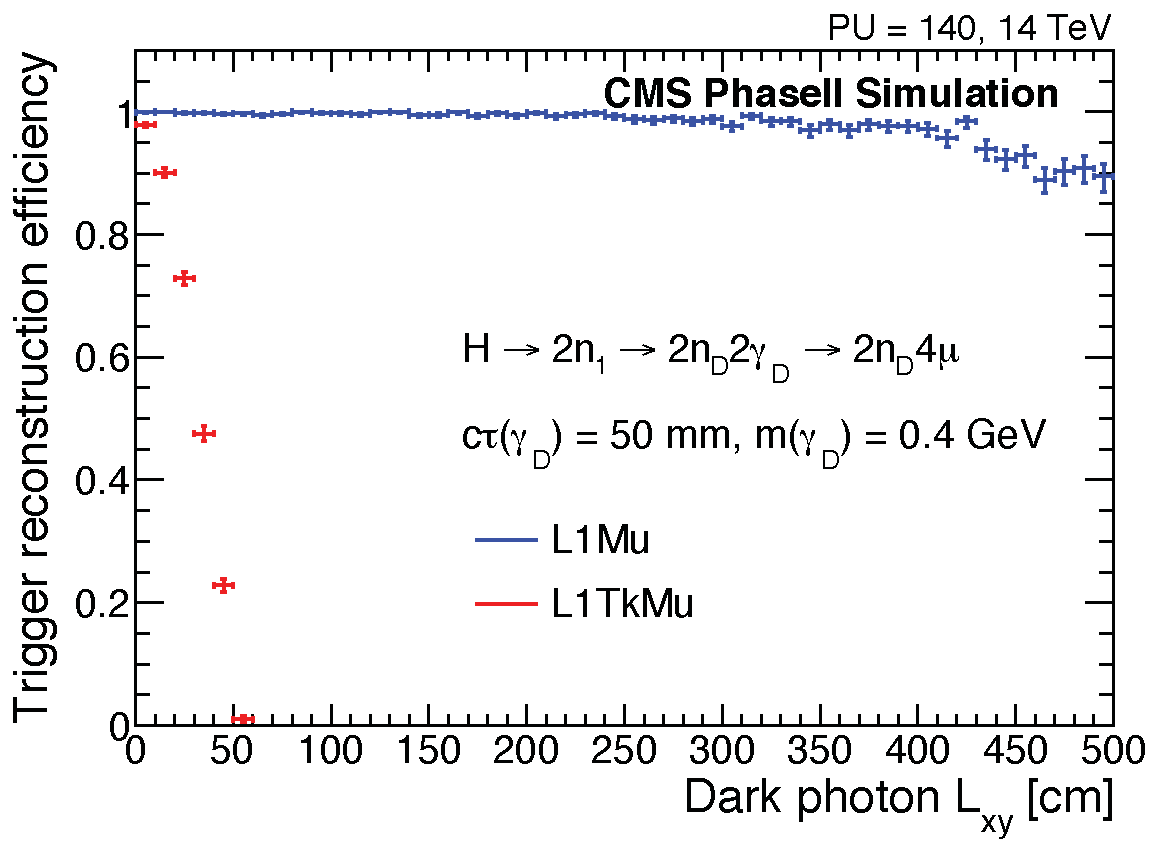
\includegraphics[width=0.6\textwidth]{img/II-1-gem/dark-photon.pdf}
      \caption{The probability of reconstructing at least one muon candidate produced in the decay of a light long-lived light particle decaying to a pair of muons $\gamma_d \rightarrow \mu \mu $ as a function of L$_{xy}$, the distance between the $\gamma_d$ decay vertex to the beamline in the transverse plane. Standalone muon trigger L1Mu performance is compared to that of L1TrkMu, a trigger based on matching muon and track trigger candidates with the CMS Phase-II detector simulation \cite{Colaleo:2021453}.}
      \label{fig:II-1-dark-photon}
    \end{figure}

  \section{Technology Overview of Triple-GEM detectors}

    A GEM foil is a 50-$\mu$m-thick polymer foil covered with 5-$\mu$m-thin copper sheets on both sides chemically perforated by a high density of microscopic holes. The polymer used is either Kapton or Apical, both with a dielectric constant of 3.5. The holes are truncated double cones with an outer diameter of 70 $\mu$m and a inner diameter of 50 $\mu$m and are spaced by 140 $\mu$m on an hexagonal grid. The structure of the GEM foil as shown on the left in Figure \ref{fig:II-1-holes}, is obtained using photolitography techniques that require precise alignment of the top and bottom masks. \\

    The diagram on the right in Figure \ref{fig:II-1-holes} represents the electric field lines that appear when a high voltage difference is applied between the two layers of copper, typically on the order of 300 V, resulting in field densities inside the holes reaching approximately 80 kV cm$^{-1}$. The structure of the electric field is used to amplify the signal of particles passing through the detector. Electrons resulting from the ionization of the gas by charged particles are directed towards the holes of the foil. When reaching high kinetic energy inside the holes, they themselves ionize the medium, producing secondary avalanches of electrons. Each hole acts as a proportional counter with gains up to 800.  \\

    \begin{figure}[h!]
      \centering
      \includegraphics[width=\textwidth]{img/II-1-gem/holes.pdf}
      \caption{Left: scanning electron microscope picture of a GEM foil. Right: schematic view of the electric field lines (white), electron flow (blue), and ion flow (purple) through a bi-conical GEM hole \cite{Colaleo:2021453}.}
      \label{fig:II-1-holes}
    \end{figure}

    To achieve high gains in the detectors, two solutions can be implemented: increase the high voltage on the foils, or use multiple foils. The first option gives rise to discharges when operating at too high electric fields thus damaging the detector. Therefore, the choice to use three GEM foils has been made, hence the name of Triple-GEM detectors. The foils are arranged as shown in Figure \ref{fig:II-1-triple}. A drift cathode is placed on the top of the chamber which creates an electric field between itself and the top copper layer of the first GEM foil in the so-called drift gap measuring 3 mm. Electrons originating from the ionization of the gas mixture (either 70\% Argon + 30\% CO$_2$ or 45\% Argon + 15\% CO$_2$ + 40\% CF$_4$) by a charged particle drift towards the holes of the foil, while ions are collected by the cathode. Following, the electron shower is amplified by GEM 1, GEM 2, and GEM 3, respectively transferring the signal to the transfer 1, transfer 2, and induction gaps measuring 1 mm, 2 mm, and 1 mm each. The size of each gap is of importance in the detector performance and has been optimized over time to increase the speed of the signal and the detector efficiency. The current configuration is called 3/1/2/1 mm in reference to the gap size. In the induction gap, the drift of the electrons towards the anodes induces a signal on the latter which can be detected by electronics. The choice to use either ArCO$_2$ or ArCO$_2$CF$_4$ has yet to be made. Although the use of CF$_4$ improves given parameters of the detector exposed bellow, CMS has limited its use due to its toxicity for the environment. \\

    \begin{figure}[h!]
      \centering
      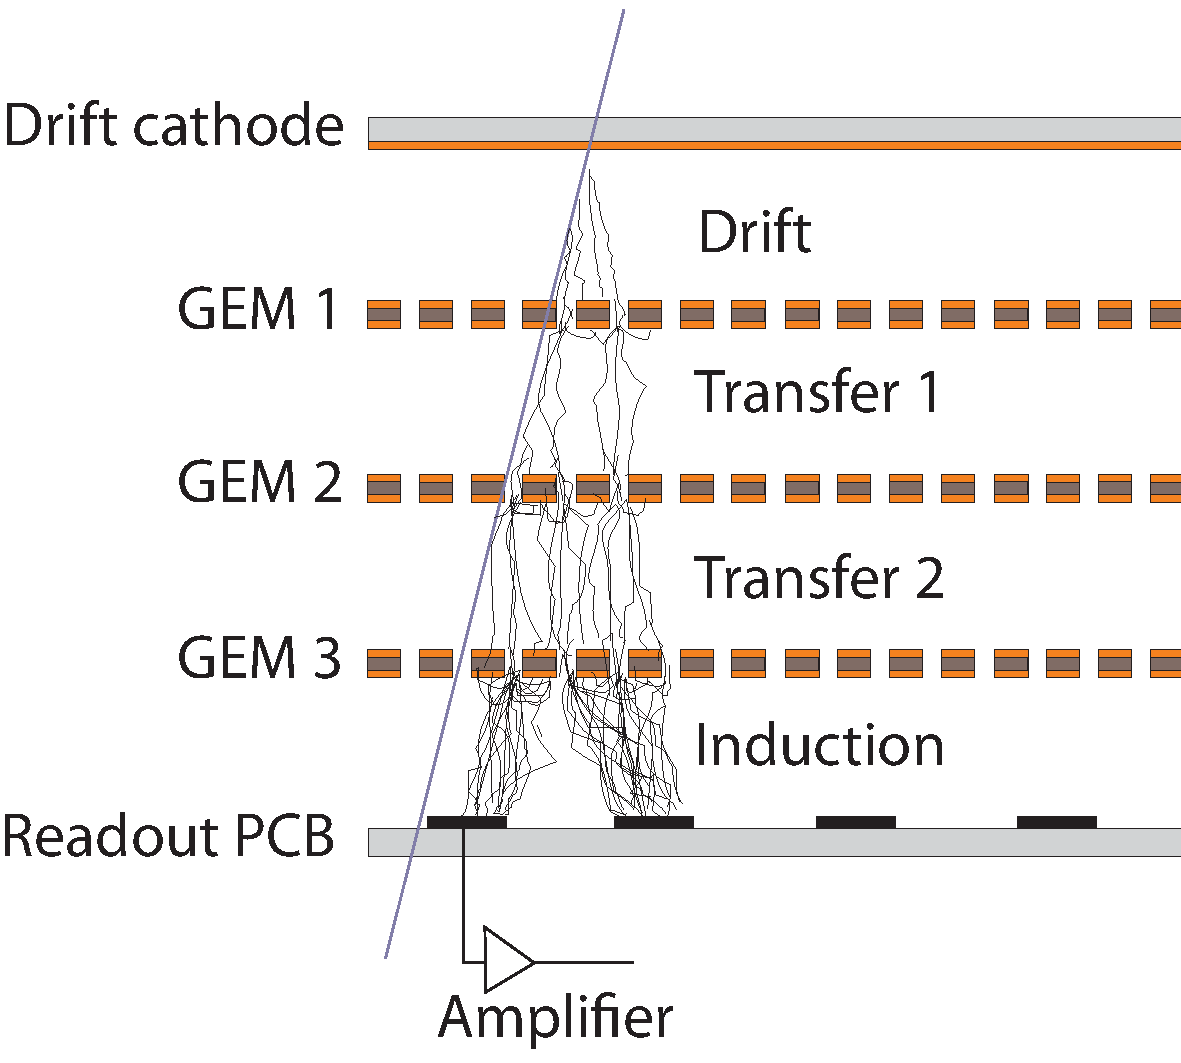
\includegraphics[width=0.5\textwidth]{img/II-1-gem/triple-gem-foils.pdf}
      \caption{Principle of operation of a generic triple-GEM chamber and definition of drift, transfer, and signal induction gap regions within the detector \cite{Colaleo:2021453}.}
      \label{fig:II-1-triple}
    \end{figure}

  \section{Technical Design of GE1/1 chambers for CMS}

    The GE1/1 chambers are arranged in pairs to form superchambers, each covering 10$^o$ in $ \phi $ for a total of 72 chambers per endcap. Figure \ref{fig:II-1-superchamber} displays the geometry of the superchambers. Due to mechanical constraint, the trapezoidal chambers are declined in two versions: a short one and a long one. The short chambers cover 1.61 < |$\eta$| < 2.18 and have a large base of 445 mm, a small base of 220 mm, and a height of 990 mm. The long chambers cover 1.55 < |$\eta$| < 2.18 and have a large base of 510 mm, a small base of 279 mm, and a height of 1283 mm. \\

    \begin{figure}[h!]
      \centering
      \includegraphics[width=0.6\textwidth]{img/II-1-gem/superchamber.pdf}
      \caption{A pair of GEM chambers form a superchamber \cite{Colaleo:2021453}.}
      \label{fig:II-1-superchamber}
    \end{figure}

    The structure of a single chamber is shown in Figure \ref{fig:II-1-exploded} which provides an exploded view of the detector. The drift cathode is placed on the bottom of the detector on which a frame is attached. The three GEM foils are stretched out using screws embedded in the frame along with the seals making the chamber air tight. The anode strips are engraved on the readout board that closes the active region of the detector. One chamber is divided into three $ \phi $ sectors and eight $ \eta $ sectors with 128 strips running radially in each. This results in a mean coverage per strip of 450 $\mu$rad and a pitch varying from approximately 500 $\mu$m to 1.3 mm. To each group of 128-strips a front-end electronics chip called the VFAT3 is attached. It digitizes the signals from the strips returning a single hit/not-hit bit. The VFAT3s are all connected to the GEM Electronics Board (GEB) which acts as router to forward the data towards the OptoHybrid, a concentrator board located on the large side of the GEM which is the interface to the off-detector electronics. The VFAT3s and the OptoHybrid are cooled down using cooling pipes attached on the top of the boards. Finally, a protective cover closes and protects the detector. When two chambers are assembled, a patch panel is added in order to facilitate the insertion and removal of the low and high voltage cables, the water for the cooling, the gas, and the optical fibers connected to the DAQ system. Note that a single source of high voltage is needed to power a chamber thanks to the use of a ceramic voltage divider which spreads the voltage over the various layers. \\

    \begin{figure}[h!]
      \centering
      \includegraphics[width=\textwidth]{img/II-1-gem/gem-exploded.pdf}
      \caption{Exploded view of the mechanical design of a Triple-GEM chamber \cite{Colaleo:2021453}.}
      \label{fig:II-1-exploded}
    \end{figure}

    Once assembled, the 72 superchambers will be installed in the endcaps of CMS as displayed in Figure \ref{fig:II-1-wheel} which shows the first station of the endcap of CMS. The full ring will be placed in the so-called nose of the endcap, between the HCAL and the ME1/1 stations.

    \begin{figure}[p]
      \centering
      \includegraphics[width=\textwidth]{img/II-1-gem/wheel.png}
      \caption{First CMS muon endcap station where the inner ring is equipped with 18 long and 18 short triple GEM superchambers \cite{Colaleo:2021453}.}
      \label{fig:II-1-wheel}
    \end{figure}

  \section{Detector Design Evolution}

    The design and fabrication method of the GE1/1 chambers has evolved over the past 5 years of R\&D. The five generations of detectors are shown in Figure \ref{fig:II-1-generations}. GE1/1-I was the first 1-m-long prototype. It was equipped with only eight readout sectors, components were glued together and GEM foils were separated using spacers. The number of sectors was increased to 24 in GE1/1-II with the full granularity of the current design (384 strips per 10$^o$). The gap configuration was changed from 3/2/2/2 mm to 3/1/2/1 mm to increase the signal speed. From GE1/1-III and onwards, GEM foils were stretched mechanically using an outer frame glued on the drift board. This design also introduced the use of a miniature ceramic high-voltage divider to apply voltage on the foils. However, the assembly of the chamber induced mechanical tension on the readout board, deforming the detector and resulting in a non-uniform response. This problem was resolved in GE1/1-IV by pre-bending the boards in the opposite direction to compensate before being bolted to the frames. This generation was the first assembled without glue, reducing production time to a few hours. However, the pre-beding technique did not yield viable results. Therefore, GE1/1-V uses pull-out pieces to tension the foils to the outer frame, on which the drift and readout board are bolted. The outer frame serves as a wall for the chamber and seals it using O-rings. Finally, the version of the design of the chambers that will be installed in CMS is GE1/1-VI which has optimized dimension to maximize the geometrical acceptance.

    \begin{figure}[h!]
      \centering
      \includegraphics[width=\textwidth]{img/II-1-gem/generations.pdf}
      \caption{Five generations of GE1/1 prototype chambers constructed and tested by the GEM collaboration in 2010-2014. The split figures for GE1/1-II and GE1/1-V demonstrate the evolution from construction using spacer frames to purely mechanical stretching of GEM foils without any spacers \cite{Colaleo:2021453}.}
      \label{fig:II-1-generations}
    \end{figure}

  \section{GE1/1 Prototyping Results}

    In order to provide the desired trigger and physics performance, the GE1/1 chambers must meet the following list of requirements:
    \begin{itemize}
      \item Maximum geometric acceptance within the given CMS envelope;
      \item Rate capability of 10 kHz cm$^{-2}$ or better to cope with the HL-LHC hit rate;
      \item Single-chamber efficiency of 97\% or better for detecting minimum ionizing particles resulting in 99.9\% efficiency for a superchamber when signals are combined with a logical OR;
      \item Angular resolution of 300 $\mu$rad or better on $ \Delta \phi = \phi_{GE1/1} - \phi_{ME1/1} $ to discriminate high-p$_T$ from low-p$_T$ muons;
      \item Timing resolution of 10 ns or better for a single chamber, which can be improved when combining the superchamber measurements, to allow matching with the CSC hits;
      \item Gain uniformity of 15\% or better across a chamber and between chambers to ensure that no geometrical or trigger biases are present. \\
    \end{itemize}

    Rate capability has been measured by monitoring the gain of a chamber when subject to a 22 keV Ag X-ray source and a high-intensity 8 keV Cu source. With Ar/CO$_2$, gain uniformity is maintained up to 100 MHz cm$^{-2}$, at which point the gain begins to drop. This confirms that the GE1/1 chambers are able to sustain rates up to 10 000 times higher than what they will experience in the 1.6 < |$\eta$| < 2.2 region of CMS. \\

    The detection efficiency is measured using a multi-layer tracking system placed in front of the detector in a beam of particles. Tracks are reconstructed in the former and extrapolated to the latter to match with reconstructed hits. When using the analog readout electronics, an offline cut is applied on the charge of the strips to cancel noise. In the digital readout system, an online threshold is applied. Both results indicate an efficiency plateau at 97\%. \\

    Using the above mentioned tracking system, the angular resolution of the GE1/1 chambers has also been measured during test beams. The resolution is taken to be the difference between the projected track position and the measured position in the detector. A resolution of 137$\pm$1 $\mu$rad has been obtained setting an upper limit on the angular resolution which is close to the theoretical value computed for a binary readout of
    \begin{equation}
      \frac{\text{angular strip pitch}}{\sqrt{12}} = \frac{455\  \mu\text{rad}}{\sqrt{12}} = 131\ \mu\text{rad} .
    \end{equation}
    Similar results were obtained using analog readout systems. \\

    The timing measurements are done by fitting the spread of the distribution plotting the time difference between a trigger seen by scintillators and the detection of the particle by the GEM detector. Time resolution studies have been performed using Ar/CO$_2$/CF$_4$ as well as Ar/CO$_2$ gas mixtures. The former yields as resolution of 4 ns due to the fast electron transport speed in CF$_4$ while the latter provides 8 ns. \\

    The response uniformity of the GEMs is measured for each detector as part of the quality control process. An X-ray generator is used to scan the entire chamber and the peak amplitude of the pulse charge distribution is taken as measurement of the uniformity. The latter does not vary more than 15\% across the detector.

  \section{GEM Upgrade Schedule}

    As previously stated, the objective of the GEM collaboration is to install a full ring of GE1/1 detectors in the first muon station of the endcaps during LS2 to maintain good trigger performances. To this end, the collaboration launched a large R\&D program to study the GEM technology and to develop a new DAQ system for the detectors which is described in details in Chapter \ref{chap:II-2-daq}. These developments have been and will be tested during test beam campaigns and in CMS to characterize the chambers and prepare the installation in CMS. \\

    Various test beam campaigns have been organized at CERN using the SPS proton beam to produce muons and pions to measure the performance of the detectors and test the developments done on the new DAQ system. The results of the latest test beam are discussed in Chapter \ref{chap:II-3-test-beam}. Besides test beams, mechanical tests have also been operated to prepare the installation of the chambers in the muon spectrometer. At the beginning of LS1, three replicas of superchambers have been installed in CMS to measure the available space and plan for cable space. \\

    At the end of 2016, during the YETS, four superchambers will be installed in CMS equipped with a full DAQ system and connected to the central DAQ of CMS. This small scale test is called the slice test and will demonstrate the integration of the GEMs with the CSCs before the full installation during LS2. As developments on the DAQ systems are still ongoing, the detectors will be equipped with slightly different components in the readout chain which are reviewed in Chapter \ref{chap:II-4-slice-test}. \\

    Finally, before installation in CMS, each component needs to be qualified, characterized, and tested against the effects of radiation. To this end, automated procedures have been developed and are described in Chapters \ref{chap:II-5-qualification} and \ref{chap:II-6-irradiation}. \\

    Beyond GE1/1, the GEM collaboration also investigates the possibility to equip the second inner muon station with GEMs through a project called GE2/1. 36 superchambers would cover a region in 1.60 < |$\eta$| < 2.46 with 1.84-m-long and 1.18-m-wide detectors. Due to the large size of the detectors, they would be segmented in eight $ \eta $ and six $ \phi $ sectors. The project is still in developments and proposed to be installed during LS3.
               % T OK - G OK
  %   \cleardoublepage
  %
  %   \chapter{The GEM and CSC Data Acquisition Systems}
\label{chap:II-2-daq}

  The installation of GEM detectors in CMS and the integration with the CSCs require the development of a new DAQ system for the GE1/1 project. The understanding of the structure of both the GEM and CSC readout chains as well as the common CMS central DAQ is of importance in the scope of this thesis. To this end, all three systems are presented in details in the sections that follow. \\

  \section{The GE1/1 Data Acquisition System}

    \subsection{The VFAT3 ASIC}

    \subsection{The GEM Electronics Board}

    \subsection{The OptoHybrid}

    \subsection{The GBT and Versatil Link}

    \subsection{The microTCA Standard}

    \subsection{The MP7 Advanced Mezzanine Card}

    \subsection{The AMC13}

    \subsection{The IPBus Protocol}

    \subsection{The XDAQ Application}

  \section{The CSC Data Acquisition System}

  \section{The CMS Central Data Acquisition System}
               % T OK
  %   \cleardoublepage
  %
    % \chapter{A Data Acquisition System for the Test Beam}
\label{chap:II-3-test-beam}

  During the ongoing process of the development of the DAQ system, the electronics has been tested in two test beams organised in Fall 2014 and Fall 2015. The first test beam, ran with the first prototype of the DAQ, aimed at proving the feasability of the architecture of the system, not focusing on data taking from the provided pion and muon beam but rather on usability. As the results were encouraging, the second version of the electronics was developped involving a complete redesign of the hardware, firmware, and software. Therefore, we will mainly focus on the second test beam, which electronics is described in the previous chapter, during which abundant data was recorded showing both excellent results for the detectors and the DAQ system. \\

  In this chapter, we present the firmware and software developments done for the DAQ system for the test beams followed by the analysis of the recorded data. First, we will present the firmware architecture of the OH and the GLIB to better understand the global layout of the system and the features that have been implemented to control the components. Then we will move on to the back-end applications developped to control and monitor the DAQ system and read out data. Finally, after a presentation of the layout of the test beam setup and its characteristics, we will show the results obtained after analysis of the recorded data.

  \section{Architecture of the OptoHybrid Firmware}

    The most important function of the OptoHybrid is to transfer data between the VFAT2s and the GLIB. Downwards, from the off-detector to the on-detector electronics, it transfers slow control requests and fast commands while upwards it sends the trigger and tracking data back to the back-end system. Next to the handling of the basic VFAT2 functionnalities, it must also handle the optical links and a couple of programmable registers which control the system. Furthermore, procedures that were previously implemented in software and required extensive computanionnal time have been moved to firmware in order to speed up the system. \\

    Although rather complex, the firmware of the OptoHybrid can be decomposed in six blocks: the fast commands, the trigger data, the tracking data, the slow control, the calibration routines, and the optical links. Eventough these blocks separatly will be presented, they are tighlty interconnected using a wishbone-like architecture for intercommunication.

    \subsection{Internal Communication Through a Wishbone-Like Architecture}

      Wishbone is an open-source communication protocol used in many projects to enable data transfer between ICs. A light version of the protocol has been implemented in the OptoHybrid to link the various modules of the system. The latter are divided in two categories: masters which initiate requests, and slaves which provide responses. The link between the two is done through a switching hub which redirects the requests to the appropriate slaves by using a 32-bit-long address space mapped to the various modules. By design, multiple masters can interact simultaneously with different slaves allowing for parrallelism in the system. \\

      A request form a master is composed of four signals: a flag signaling the presence of a request, a write-enable bit to indicate the nature of the request (read or write), a 32-bit-long address to which the request will be redirected, and an optionnal 32-bit-long data field in case the request is a write operation. The response from a slave consists of: an ackownledgment signal, a 4-bit-long error status in case the operation failed, and an optionnal 32-bit-long data field holding the response to read requests. A programmable timeout has also been implemented to avoir blocking operation. Some components implement both a master and a slave module in order to be able to receive requests and propagate them to various other modules. \\

      Communication done through the wishbone-like protocol is used mainly for slow control or non-time-critical operations as the latency of a transaction is not fixed. Indeed, the switching hub implements a waiting list functionnality which allows two masters to address the same slave at the same time by storing one of the requests in memory and awaiting for the slave to finish the other transaction.

    \subsection{Encoding Fast Commands}

      Fast commands such as L1As, Resyncs, BC0s, etc can originate from various sources. In normal data taking runs, the AMC13 receives the TTC signals, forwards them to the microTCA AMC which in turn transmits them to the OptoHybrid. When data taking is stopped and calibration runs are performed, the routines implemented in the OptoHybrid are ran and require fast commands. To this end, the TTC signals can also be generated locally using the T1 generator block. This entity can generate L1As, Resyncs, BC0s, and CalPulses in three different ways: send a single command a given number of times at fixed interval, send a CalPulse followed by a L1A with a fixed delay, or send a programmable pattern involving all the commands. Finally, the two remaining sources of TTC commands, and more precisly L1As, are either a loopback from a given VFAT2 trigger bits directly to all the VFAT2s (self-triggering) or the signals coming from an external component through a debugging header on the OptoHybrid. \\

      The switching between the various sources is done by setting a register through slow control operations. Once the source has been selected, the commands are forwarded to the VFAT2s and encoded on the T1 signals. Each command is composed of three bits clocked at 40 MHz. An additionnal feature has been added to the L1A line to throttle the trigger signals when working in high rate environments. Through registers, the operator can select to send only a fraction of the received commands to not overload the VFAT2 buffers and allow for correct readout of the chip.

    \subsection{Formatting Trigger Data}

      Each of the 24 VFAT2s transmits eight trigger bits per BX. These are regroupped using a logic OR in the DAQ system of the test beam  thus yielding 24 bits. The trigger information is used for calibration routines and forwarded over debugging headers to an external electronics crate. As the number of external connections is limited, only six trigger bits can be send thus requiring the need for a selection mechanism controller by programmable registers.

    \subsection{Acquiring Tracking Data}

      Upon reception of a L1A, the VFAT2 transfers the selected event from its SRAM1 to SRAM2 and then to an encoder which serialises the data. Each event is 192 bits long followed by two idle bits and clocked at 40 MHz. This means that it takes 194 BXs to read out one event and that the VFAT2 cannot handle trigger rates higher than $\approx$ 200 kHz without experiencing an overflow of the buffers. The data is pushed out of the VFAT2 automatically and formatted according to the pattern shown in Table \ref{tab:II-3-test-beam-vfat2-tk-format}. The top left bits are Most Significant Bits (MSBs) which are pushed out first and the bottom right bits or the Least Significant Bits (LSBs) which come in last. The first four bits of the first three 16-bit-long words are constant values. These are completed by the BC which increments at each clock cycle, the EC which counts the number of received L1As, four flags which hold information on the status of the buffers, and a chip ID unique to each VFAT2. Following are the 128 bits reflecting the hit information on each channel. Finally, the VFAT2 uses a Cyclic Redundancy Check (CRC) on 16 bits to detect errors. The CRC uses all other 176 bits to encode its data but does not provide a way to correct errors. \\

      \begin{table}
        \begin{tabularx}{\textwidth}{C{1}}
          \textbf{VFAT2 tracking data} \\
          {
          \begin{tabularx}{0.5\textwidth}{|C{1}|C{1}|C{1}|}
            \hline
            \multicolumn{3}{|c|}{15 \hfill 0} \\ \hline
            1010 & \multicolumn{2}{|c|}{BC[11:0]} \\ \hline
            1100 & EC[7:0] & Flags[3:0] \\ \hline
            1110 & \multicolumn{2}{|c|}{Chip ID[11:0]} \\ \hline
            \multicolumn{3}{|c|}{Channel data x8} \\ \hline
            \multicolumn{3}{|c|}{CRC} \\ \hline
          \end{tabularx} }
        \end{tabularx}
        \caption{??}
        \label{tab:II-3-test-beam-vfat2-tk-format}
      \end{table}

      Next to the data line, each VFAT2 provides a DataValid line which is pulled high when the bits coming out of the VFAT2 are valid. However, due to the limited number of pins connecting the GEB and the OptoHybrid, this signal has been left unconnected for all but six VFAT2s. Therefore, data is constantly shifted in a 194 bits (192 bits of data and 2 idle bits) serial-to-parrallel converter and analyzed. When the fixed pattern of 12 bits is seen, a flag is raised signaling the presence of potential data. The data packet is split up in its various elements and the CRC is recomputed and compared against the received CRC. Two additionnal flags respectivly hold the results of the comparation of both CRCs indicating if the data is valid or not, and a logic OR of all 128 channel to indicate if the packet contains a hit or not. In theory, only packets with valid CRCs could be transmitted to the back-end electronics. However, sending all packets offer the possibility to identify recurring errors in the CRCs computation and offers the possibility to correct them offline. \\

      In parallel to the decoding of the data packets, the OptoHybrid maintains its own BC and stores the value of the counter in a buffer each time a L1A is received. When the decoding modules report they have detected data, a concentrator module aggragates the information from all available VFAT2s. Every packet received within a window of 10 BX is assigned to the same event to which the value of the corresponding BC is appended. The assembled event is stored in a large buffer to be latter sent over the optical links to the GLIB. \\

      To prevent positions either not equipped with VFAT2 Hybrids or that are noisy to generate fake data, a 24-bit-long register allows to mask individual positions to ignore any packets it generates. Next to this, each decoding module is equipped with two counter respectivly counting the number of valid and invalid packets.

    \subsection{Controlling and Monitoring the Systems}

      The OptoHybrid is used to control itself through wishbone and the VFAT2s through I2C. The slow control of the OptoHybrid mainly consists in selecting TTC command sources, setting the trigger throttling, reading out counters, etc. These operations are performed to control the data flow and the functionning of the DAQ system itself. Commands sent to the VFAT2s on the other hand have direct impact on the physics of the data taking through the biais of the analog front-end readout. \\

      To communicate with the VFAT2s, six I2C controllers are implemented in the firmware of the OptoHybrid, one per sector on the GEB. Each controller can access four VFAT2s which are identified using three resistors that can be installed on the GEB. VFAT2 uses a modified I2C protocol which uses the same frame format as the official one but a different addressing scheme. The official I2C data frame is shown in Figure \ref{fig:II-3-test-beam-i2c}. The master starts by sending seven address bits which are used to identify the slave it wants to talk to, followed by a read/write bit. After the slave acknowledged the request, eight bits are sent from the master to the slave in case of a write operation followed by a slave acknowledgment, or the opposite in case of a read operation. For the VFAT2, the first three bits of the address are used to select the chip that is addressed by the master while the four remeaning bits are used to select the register that needs to be accessed. This addressing scheme allows the OptoHybrid to access up to 16 registers on the VFAT2s. However, each VFAT2 holds 16 primary registers and 136 extended registers. The extended registers are accesses using two primary pointer registers: one set to point to an extended register, and one to read/write the data in said register. Thus, in order to perform a transaction on a primary register, only one operation is necessary, while two are required to access extended registers. \\

      \begin{figure}[h!]
        \centering
        \includegraphics[width=\textwidth]{img/II-3-test-beam/i2c.png}
        \caption{??? \cite{I2C}.}
        \label{fig:II-3-test-beam-i2c}
      \end{figure}

      To make this process transparent to the user and flatten out the address space of the VFAT2s, the OptoHybrid maps the primary registers from addresses 0 to 16 and the extended registers from addresses 17 to 152. When performing a transaction with the extended registers, the I2C controllers automatically run the double addressing scheme. \\

      Next to the basic I2C controllers, an extended I2C controller was developped to abstract individual addressing and allow request broadcasting. This module forwards I2C requests to all selected VFAT2s at once to configure the entire system in parallel. A programmable register allows to leave out given VFAT2s from the broadcast while a buffer stores the result of the operations.

    \subsection{Calibrating the Systems}

      The calibration routines have been ported from software to firmware in order to increase their speed of operation and reduce the number of requests that need to be performed. The routines are as follows: a threshold scan which measures the noise on the strips as a function of the threshold of the VFAT2s, a latency scan which allows to select the correct BX when receiving L1As, and a s-curve scan which characterize the response of the strips as a function of the collected charge and threshold. \\

      \paragraph{The threshold scan} is used to scan each VFAT2 for noise. For each threshold value set on the VFAT2, the percentage of events displaying a hit is recorded and taken as the percentage of noise. A graph can be obtained showing the noise decrease as the threshold increases yielding a point at which the system can be operated with minimal noise. The threshold scan can be operated using trigger information on the 128 strips as a whole or on individual strips using tracking data. For the latter, the T1 generator is used as trigger source to generate data as these runs being performed when the beam is off. No relation between a L1A and physical event is needed to study the noise on the system. \\

      \paragraph{The latency scan} allows to determine the best latency value to be set in a VFAT2. The latency is the time difference, in number of BX, between the time of arrival of a L1A and the time at which the related event was stored in the VFAT2 buffer. This module is operated when the particle beam is on and triggers are generated by an external source such as a Photomultiplier (PM) placed in front of the detector. For each value of the latency, the OptoHybrid counts the ratio of events with hits over the total number of events. For a noiseless VFAT2 with 100\% detection efficiency, the ratio would be 0\% outside the correct latency window and 100\% inside. The size of the window can be adjusted by changing the length of the monostables output in the VFAT2s. \\

      \paragraph{The s-curve scan} is part of the calibration routines performed for the qualification of the VFAT2s. It yields the response of the VFAT2 strips to an injected charge pulse according to the threshold. It is used in conjunction with the T1 generator which send a CalPulse followed by a L1A at fixed interval, thus with known latency. The use and results obtained for this module are further detailled in Chapter \ref{chap:II-5-qualification}.

    \subsection{Optical Communication with the Off-Detector Electronics}

      The link between the OptoHybrid and the off-detector electronics are the optical links from which two are used: one for the trigger data and fast commands, and one for the tracking data and slow control. Each optical fibre is connected to an SFP+ transceiver which contains the Light Emitting Diode (LED) that drives the link. The SFP+ module is in turn connected to a Gigabit Transceiver X (GTX) block inside the FPGA which is a dedicated component that can handle high-speed serial communications.

      \paragraph{The GTX module} is in charge of the serialization/deserialization of high-speed data. A schematic diagram of the functions it provides ir shown in Figure \ref{fig:II-3-test-beam-gtx}. The GTX handles both the transmission and reception of data. From the FPGA logic, it receives a parallel vector of bits containing the raw data. The raw data enters the Transmit FIFO which acts as a buffer before the Line Encoding module. The latter uses an eight-bit/ten-bit (8b/10b) encoding scheming which is a standard in high-speed communications. 8b/10b encodes every eight bit word on ten bits according to a predefined table. It has the particularity that whatever combination of words might be sent, no more than five successive '0's or '1's will arise in the serial stream. This ensures line balancing: the fact that the electric lines between the GTX and the SFP+ module will remain at an average voltage and not drift to a logic '1' or '0' over time, thus requiring a longer fall or rise time of the signals. 8b/10b also offers a set of K-characters which are unique patterns of bit that can never arise randomly in the stream. Those characters are used to detect the beginning of a frame and allow the receiver to align correctly. Finally, after the encoding of the data frame is done, it is serialized and transmitted to the SFP+ module over differential pairs. \\

      \begin{figure}[h!]
        \centering
        \includegraphics[width=\textwidth]{img/II-3-test-beam/gtx.png}
        \caption{??? \cite{GTX}.}
        \label{fig:II-3-test-beam-gtx}
      \end{figure}

      The receiver essentially follows the opposite path as the transmitter except for the Clock Managment block. The 8b/10b encoding offers one more advantage which is the possibility to recover a clock from the data stream itself, technique called Clock Data Recovery (CDR). In high-speed signal design, small variations in the clock frequency between the transmitter and the receiver can lead to discrepancy in the read out data. To avoid this, the receiver can tune the frequency of the clock of its deserializer using the transitions of the bits in the incoming stream to align its phase to the data. The GTX block further provides the obtained recovered clock to the FPGA to use in the logic. Correct alignment of the data is checked using the K-characters in the stream.

      \paragraph{The fixed latency link} is used to transmit trigger data from the OptoHybrid to the GLIB and receive the fast commands. Of the 64 bits that the downlink transmits, 16 are used to align the serial bit stream on the receiving side and four others are used to encode the four fast commands that the VFAT2 understands. The other 44 bits are not used and left to constant zeros. The uplink uses a 16 bit header to align the stream to which it appends the 24 triggers bits coming from the logic-OR of the VFAT2s. These patterns repeat at 40 MHz as data changes every BX.

      \paragraph{The variable latency link} is used to transmit and receive slow control commands and to transmit the tracking data of one VFAT2 at the time to the GLIB. As only one VFAT2 was exposed to the beam at any given time during the test beam, reconstructing and sending the full event was not a necessity for the DAQ system. In both directions, a given frame format is constantly sent using two bits in the header to indicate the presence of a valid slow control request and valid VFAT2 tracking data in case of the uplink. The two data formats are shown in Table \ref{tab:II-3-test-beam-data-format}. Both send a 16 bit header to align the link followed by the frame data. As can be seen in the table on the left, the OptoHybrid receives requests from the optical link which are then converted to wishbone-like requests by the logic. The optical link module is one of the wishbone masters that controls the system and which responses are forwarded back to the GLIB.

      \begin{table}
        \begin{tabularx}{\textwidth}{C{1}C{1}}
          \textbf{GLIB to OptoHybrid frame} & \textbf{OptoHybrid to GLIB frame} \\
          {
          \begin{tabularx}{0.4\textwidth}{|C{1}|}
            \hline
            15 \hfill 0 \\ \hline
            Header \\ \hline
            Request address (MSB) \\ \hline
            Request address (LSB) \\ \hline
            Request data (MSB) \\ \hline
            Request data (LSB) \\ \hline
            CRC \\ \hline
          \end{tabularx} }
          &
          { \begin{tabularx}{0.4\textwidth}{|C{1}|}
            \hline
            15 \hfill 0 \\ \hline
            Header \\ \hline
            VFAT2 data x14 \\ \hline
            Response data (MSB) \\ \hline
            Response data (LSB) \\ \hline
            CRC \\ \hline
          \end{tabularx} }
        \end{tabularx}
        \caption{??}
        \label{tab:II-3-test-beam-data-format}
      \end{table}

  \section{Architecture of the GLIB Firmware}

  \section{The Control and Monitoring Application}

  \section{The Test Beam Setup}

  \section{Analysis of the Collected Data}



























  -
        % T OK - G OK
    % \cleardoublepage
  %
  %   \chapter{Qualification of the Electronics}
\label{chap:II-4-qualification}

  To prepare the DAQ system for the slice test, the electronic components need to be tested and qualified. For the VFAT2s, qualification procedures have to be developed to characterize the analog front-end of each chip, record their response to calibration pulses, and optimize the parameters to achieve uniformity over the entire detector. For the GEB, qualification means ensuring that no shorts are present and that the integrity of the signals is kept over the full length of the board. Finally, the system as a whole needs to be tested against communication errors or readout problems. \\

  In this chapter, we present the algorithms we have developed to test and qualify the various systems which rely on the firmware and software development made for the test beam. We detail the calibration procedure of the analog front-end of the VFAT2 which has never been done before. Next, we describe the GEB testing PCB which we have created in order to test the communication through the GEB. Finally, we talk about the script used to test the system as a whole which is employed at CERN and in various research laboratories to set up DAQ systems for future developments.

  \section{Qualification of the VFAT2s}

    The qualification process of the VFAT2s has been automatized using Python scripts relying on IPBus to run the various procedures using the dedicated firmware modules of the OptoHybrid. The aim of this tools is to reject faulty chips and record the parameters of the analog front-end which slightly vary from component to component.

    \subsection{Identification of Faulty Channels}

      The first step of the procedure is to run a threshold scan for each channel to reveal those that are not responding or that are noisy. To do so, the tools use the threshold scan module of the firmware that relies on tracking data to access the full granularity information. Figure \ref{fig:II-4-threshold} is a two-dimensional graph plotting the evolution of the noise level for each channel as a function of the VFAT2 threshold in VFAT2 units. As can be seen, one of the channels appears to be damaged as it does not display any change during the whole scan and remains empty. From this result, the VFAT2 would be disqualified and not used for data taking. If performing these scans on instrumented VFAT2s, the results can be used to mask faulty channels and regain acceptable operational conditions.

      \begin{figure}[h!]
        \centering
        \includegraphics[width=0.5\textwidth]{img/plots/cThreshold_Channel-crop}
        \caption{Two-dimensional graph plotting the evolution of the noise level for each channel as a function of the VFAT2 threshold in VFAT2 units.}
        \label{fig:II-4-threshold}
      \end{figure}

    \subsection{Front-end Currents and Voltages}

      Following the threshold scan, the procedure reads out the currents and voltages that are produced by the VFAT2 to bias its analog front-end. When writing values in the 8-bit registers defining the threshold and other parameters, a conversion to an analog value is performed inside the chip which will vary from component to component. It is therefore essential to record the results of each chip. In order to access the analog signals inside the VFAT2, two analog signals are sent out: one for the voltage reference and one for the current reference. These lines are routed on the GEB and transmitted to the OptoHybrid which uses an analog-to-digital converter (ADC) to digitize the information. To fit the window of operation of the ADC, which has a range of 0 V to 1 V, the voltage signal is sent through a voltage divider and the current signal is measured over a resistor. Figure \ref{fig:II-4-adc} plots the ADC counts, current values on the left, and voltage values on the right of each settable register of the VFAT2 as a function of the 8-bit value written in the register. \\

      \begin{figure}[h!]
        \centering
        \includegraphics[width=0.49\textwidth]{img/plots/cADC_Current-crop}
        \includegraphics[width=0.49\textwidth]{img/plots/cADC_Voltage-crop}
        \caption{Plots of the ADC counts, current values on the left, and voltage values on the right of each settable register of the VFAT2 as a function of the 8-bit value written in the register.}
        \label{fig:II-4-adc}
      \end{figure}

      All but one of the current based registers are related to the amplification and shaping of the analog signal. They power the front-end and are used to define the length of the tail of the signal shape, the rise time of the distribution, etc. The remaining register, IComp, defines the amount of current delivered to the comparator which in turn influences the response time of the later. These parameters are set to default values provided by the reference manual of the VFAT2. \\

      The voltage base registers are used for the comparator and the calibration modules. The VThreshold1 and VThreshold2 signals are those defining the threshold on the strips. By design, VFAT2 can handle positive and negative pulse and provides one threshold register for each polarity. During operations, one of the registers is set to zero and the other one is used to adjust the threshold, meaning that a single parameter is used. The VBaseline, VCal, and VLow registers are used to define the amplitude of the calibration pulse sent to the channels. Figure \ref{fig:II-4-injection} shows a diagram of the injection and calibration circuit of the VFAT2. The amplitude of the calibration pulse is equal to the difference between VBaseline which has a fixed value and VLow which is programmable. The output pulse is sent to one channel over a capacitor of 100 fF resulting in a pulse amplitude in term of charge of
      \begin{equation}
        Q = 100 \ \text{fF} \times \left(\text{VBaseline} - \text{VLow} \right) .
      \end{equation}

      \begin{figure}[h!]
        \centering
        \includegraphics[width=0.8\textwidth]{img/II-4-qualification/injection.png}
        \caption{Diagram of the injection and calibration circuit of the VFAT2 highlighting the path of the calibration pulse towards a given channel \cite{Aspell:1267947}.}
        \label{fig:II-4-injection}
      \end{figure}

    \subsection{Front-end Calibration}

      Using the results from the ADC, the script can determine what amount of charge is injected during the calibration phase of the VFAT2 upon reception of a CalPulse fast command. With this, it is possible to produce s-curves which for a given threshold indicate at which amplitude of the calibration pulse a signal becomes visible. Figure \ref{fig:II-4-scurve} plots the hit-to-event ratio as a function of the calibration pulse height in VFAT2 units for a threshold of 25. The graph shows that below a value of 40 no signal is detected due to the threshold level. The turn-on of the curve is defined as the value for which 50\% of hit-to-event ratio is reached and is in this case equal to 44. \\

      \begin{figure}[h!]
        \centering
        \includegraphics[width=0.5\textwidth]{img/plots/cSCurve_T25-crop}
        \caption{Plot of the hit-to-event ratio as a function of the calibration pulse height in VFAT2 units for a threshold of 25.}
        \label{fig:II-4-scurve}
      \end{figure}

      The operation is then repeated for various threshold values and the turn-on value is extracted automatically using a logistic function to fit the curve. The equation of the function is as follows
      \begin{equation}
        f(x) = \frac{1}{1 + e^{-k \left( x - x_0 \right)}}
      \end{equation}
      where $ x_0 $ is the value of the midpoint or turn-on, and $ k $ is the steepness of the slope. Figure \ref{fig:II-4-scurves} is a collection of s-curve scans for various thresholds on the left which can be translated to a plot of the calibration pulse height of the turn-on in VFAT2 units and current as a function of the threshold in VFAT2 units on the right. \\

      \begin{figure}[h!]
        \centering
        \includegraphics[width=0.49\textwidth]{img/plots/cSCurve_ThresholdVCal-crop}
        \includegraphics[width=0.49\textwidth]{img/plots/cSCurve_TurnOn-crop}
        \caption{Left: collection of s-curve scans for various thresholds with corresponding curent values. Right: plot of the calibration pulse height of the turn-on in VFAT2 units and current as a function of the threshold in VFAT2 units.}
        \label{fig:II-4-scurves}
      \end{figure}

      Using these results, the threshold value applied on the strips can be converted to a charge, which is of important to compute the equivalent noise charge of the system. This is the amplitude of the noise in terms of electrons, which can easily be compared to the signal induced by the particles which is often expressed in fentocoulombs. The results presented here above are in agreement with those obtained during the initial qualification of the VFAT2 \cite{Aspell:1267947} both displaying a charge range of -2 fC to 18 fC.

    \subsection{Front-end equalization}

      The results obtained in the previous procedures were values averaged on all the strips. However, channels display a dispersion around the central value which induces a bias as the effective threshold is not constant across the chip. To eliminate this effect, it is possible to equalize the response of the front-end by using channel by channel programmable registers. Each of them is equipped with a programmable register which adjusts the threshold value slightly. The equalization procedure used to align the front-ends starts by applying a given value to the common threshold register and sets all channel registers to zero. It then performs s-curve scans for each channel. The operation is repeated but with the channel registers set to their maximum value. Figure \ref{fig:II-4-trim} plots the s-curve scans for each channel with the minimum value of the channel registers on the left and the maximum value on the right. The two plots obtained this way are very similar with only the turn-on value changing. \\

      \begin{figure}[h!]
        \centering
        \includegraphics[width=0.49\textwidth]{img/plots/cSCurve_ChannelVCal_Trim0-crop}
        \includegraphics[width=0.49\textwidth]{img/plots/cSCurve_ChannelVCal_Trim1-crop}
        \caption{Plots of the s-curve scans for each channel with the minimum value of the channel registers on the left and the maximum value on the right.}
        \label{fig:II-4-trim}
      \end{figure}

      To align the channels, the average value of turn-on for both minimal and maximal value configuration is taken and set to be the aim of the equalization routine. For each channel, the script then sets its individual register value to the mean value and performs an s-curve scan. According to the turn-on value, the register is incremented or decremented and the procedure is repeated until the channel is aligned. The results of the alignment are shown in Figure \ref{fig:II-4-trimed} which plots the s-curve scan for each channel with the aligned values for the register on the left and the dispersion of the turn-on value for the non-aligned and aligned configurations. \\

      \begin{figure}[h!]
        \centering
        \includegraphics[width=0.49\textwidth]{img/plots/cSCurve_ChannelVCal_Trimed-crop}
        \includegraphics[width=0.49\textwidth]{img/plots/cSCurve_ChannelVCal_Disp-crop}
        \caption{Left: plot of the s-curve scan for each channel with the aligned values for the channel register. Right: dispersion of the turn-on value for the non-aligned (orange and blue) and aligned configurations (green, scaled by a factor of 0.35).}
        \label{fig:II-4-trimed}
      \end{figure}

      At the end of the script, the VFAT2 channels have all been tested against noise issues and have been adjusted so that they all display the same response to calibration pulses. This is the first time the full range of possibilities offered by the VFAT2 is used in a DAQ system and demonstrates that these features are within working specification.

  \section{Qualification of the GEB}

    In order to test the GEB, a small PCB equipped with the same connector as the VFAT2 Hybrids was developed. Using signals originating from the OptoHybrid, the board can check the integrity of the data and use on-board LEDs to indicate the results of the tests for the current position.

    \subsection{The GEB Testing Board}

      The PCB is a four layer board equipped with an FPGA and microcontroller unit (MCU) to analyze the signals. Figure \ref{fig:II-4-geb-pcb} provides 3D models and a PCB layout of the board. Next to the processing units, the board also embarks an ADC, a digital-to-analog converter (DAC), a flash memory, a USB-to-SPI converter to link the universal serial bus (USB) port to the FPGA through serial peripheral interface bus (SPI), and powering options.

      \begin{figure}[h!]
        \centering
        \includegraphics[width=0.49\textwidth]{img/II-4-qualification/geb-3d-0.png}
        \includegraphics[width=0.49\textwidth]{img/II-4-qualification/geb-3d-1.png}
        \vspace*{0.3cm}
        \includegraphics[width=0.49\textwidth]{img/II-4-qualification/geb-3d-2.png}
        \includegraphics[width=0.49\textwidth]{img/II-4-qualification/geb-pcb.png}
        \caption{3D models and PCB layout of the GEB testing board.}
        \label{fig:II-4-geb-pcb}
      \end{figure}

      \paragraph{Powering of the board} is done either through the GEB connector which provides 2.5 V to the system or through the USB port. In case USB is used, the GEB power source is automatically disabled and 3.3 V is given to the system to increase processing speed. The 2.5 V or 3.3 V are further used to generate the 1.2 V required for the internal logic of the FPGA.

      \paragraph{The processing units} of the board, namely the Xilinx Spartan-6 FPGA (XC6SLX9-2TQG144C) and the ATMEL MCU (ATmega164PA), are what control the various components. The FPGA is the main element of the board and is connected to all other chips. It can either control them directly or act as a router for the signals originating from the MCU. The communication between the two processing units is done four serial buses: two universal asynchronous receiver/transmitter (UART), one SPI, and one bus composed of four GPIOs. Next to the links to the FPGA, the remaining 16 IOs of the MCU are broken out on header connectors for debugging purposes. The same is done for 22 IOs of the FPGA which are connected to headers.

      \paragraph{The GEB connector} holds 30 digital signals, 2 analog signals, and power and ground lines. The digital signals are all connected to the FPGA while the two analog signals are connected to the DAC.

      \paragraph{The USB port} is used to communicate with a computer using an FTDI chip (FT220XS) which converts the USB protocol to SPI.

      \paragraph{The analog part} of the board is controlled by the ADC (ADS1015) and the DAC (DAC8532). The two outputs of the DAC are connected to the GEB connector to drive the two analog signals digitized by the OptoHybrid. The ADC signals on the other hand are purely used for debugging purposes and connected to headers.

      \paragraph{Programming} the system is done through the Joint Test Action Group (JTAG) protocol which connects to the FPGA and the MCU. JTAG allows multiple devices to be connected in series and programs them both by shifting the configuration from one to another. The configuration scheme of the system can be modified to only affect the FPGA by removing a 0 $\Omega$ resistor which bypasses the MCU.

    \subsection{Testing the GEB}

      To test the GEB positions, the OptoHybrid is used to generate a pseudorandom binary sequence (PRBS) and transmit it over the data lines along with a reference clock. PRBS is often used to detect errors on communication lines including optical fibers. It relies on a sequence of bits to compute the next bit in the stream. A vector of bits is loaded in shift registers and is moved by one position every clock cycle. The overflowing position in transmitted on the line while the entering position is computed by summing the data stored in given positions. PRBS-7, for example, uses 7-bit-long vectors and computes the new element with
      \begin{equation}
        x_0 = x_6 XOR x_5 AND 1
      \end{equation}
      which yields a repetition period of pattern of 127 clock cycles. \\

      For each differential pair or single ended signal, a different seed is used for the PRBS-7 generator. By receiving the clock along with the data, the GEB tester board can decode the bit streams and ensure that the encoding is correct. In case one of the lines is faulty, the LEDs connected to the FPGA are used to display an error code. \\

      The analog lines are tested by generating a given voltage using the DAC. The OptoHybrid is then used to readout the value on the line and check the results are matching.

  \section{Qualification of the System}

    The final qualification procedure developed aims at testing the system in its entirety. Figure \ref{fig:II-4-script} provides a screen shot of the output of the script. The latter first attempts to establish communication with the GLIB and the OptoHybrid in section A and B. It then performs a series of read/write operations on the registers ensuring that every request receives a response in section C and D. Once the tests on the GLIB and OptoHybrid are done, the script detects all present VFAT2s in section E through I2C requests. Using these, random read/write operation are made on the registers of the VFAT2s in section F to test the reliability of the communication. Afterwards, in section G, chips are turned on one by one and tracking data is read out. The script verifies that the counters add up and that the data is not corrupted. Then, it performs the same action with all VFAT2s active at the same time in section H. The last test performed using the VFAT2s, in section I, is the maximum readout rate that can be achieved by the system. Finally, section J looks at the error rate on the optical links to ensure no errors appear on the communication lines. \\

    This test is used to test the system configuration and ensure that every component is configured correctly. It can detect errors at any level of the system, from the VFAT2s to the GLIB.

    \begin{figure}[p!]
      { \footnotesize
\begin{alltt}
A. Testing the GLIB's presence
   Trying to read the GLIB board ID... If this test fails, the script
   will stop.
   > { \color{green} Passed... }

B. Testing the OH's presence
   Trying to set the OptoHybrid registers... If this test fails, the
   script will stop.
   > { \color{green} Passed... }

C. Testing the GLIB registers
   Performing single and FIFO reads on the GLIB counters and ensuring
   they increment.
   > { \color{green} Passed... }

D. Testing the OH registers
   Performing single and FIFO reads on the OptoHybrid counters and
   ensuring they increment.
   > { \color{green} Passed... }

E. Detecting the VFAT2s over I2C
   Detecting VFAT2s on the GEM by reading out their chip ID.
   Detected 18 VFAT2s: [1, ..., 23]

F. Testing the I2C communication with the VFAT2s
   Performing random read/write operation on each connect VFAT2.
   > { \color{green} Passed... #1 }
   { \color{gray} [...] }
   > { \color{green} Passed... #23 }

G. Reading out tracking data
   Sending triggers and testing if the Event Counter adds up.
   > { \color{green} Passed... #1 }
   { \color{gray} [...] }
   > { \color{green} Passed... #23 }

H. Reading out tracking data
   Turning on all VFAT2s and looking that all the Event Counters add up.
   > { \color{green} Passed... }

I. Testing the tracking data readout rate
   Sending triggers at a given rate and looking at the maximum readout
   rate that can be achieved.
   Maximum readout rate 200000 Hz

J. Testing the optical link error rate
   GLIB tracking link error rate is of          0 Hz
   GLIB trigger link error rate is of           0 Hz
   OptoHybrid tracking link error rate is of    0 Hz
   OptoHybrid trigger link error rate is of     0 Hz

K. Results
   A.    > { \color{green} Passed... }
   { \color{gray} [...] }
   J.    > { \color{green} Passed... }
\end{alltt} }
      \caption{Output of the qualification procedure developed to test the DAQ system in its entirety.}
      \label{fig:II-4-script}
    \end{figure}

  \section{Conclusion}

    For the first time, a method was developed to use the VFAT2 capabilities to their full extend by taking advantage of the channel by channel optimization. The procedure is used to detect faulty units and perform qualification tests which results are stored in database for future reference. With this script, the analog front-end of each VFAT2 is entirely characterized which provides information on the effective threshold applied in terms of electrons and thus induced charge. \\

    Furthermore, a GEB testing board has been design to test each position on the GEB and detect broken lines. The board relies on an FPGA coupled with an MCU to communicate with the OptoHybrid and test the integrity of the transmitted signals. The results of each test are displayed using on-board LEDs. \\

    Finally, the system as a whole is tested using a script which targets specific components of the architectures. Random read/write operations to the GLIB, OptoHybrid, and VFAT2s are performed, tracking data is read out, and stress tests are done to push the system to the limit. \\

    These tools are used for the preparation of the slice test to select appropriate components and install testing facilities at CERN and in other associated research laboratories.
    % T OK
  %   \cleardoublepage
  %
    \chapter{Irradiation Tests}
\label{chap:II-5-irradiation}

  The OptoHybrid will be located in a region of CMS exposed to fluxes of particles up to 200 kHz cm$^{-2}$, some of which might interact with the FPGA and cause errors in the logic. Those could in turn influence the functioning of the system and degrade its performance. To understand and potentially solve this issue, irradiation tests have been performed to measure the interaction cross section of the particles with the various components of the FPGA. Two OptoHybrids v2a programmed with a dedicated firmware designed to detect errors have been placed in a high intensity proton beam of fluxes up to 2 $ \times $ 10$^8$ particles cm$^{-2}$ s$^{-1}$. The two boards were each controlled by an additional OptoHybrid placed outside the test area which recorded the events and statistics. \\

  In this chapter, we provide the reader with an overview of the internal architecture of an FPGA to better understand the potential sources of errors and the effects of radiation. We then describe the firmware of the irradiated and control FPGAs which has been used during the test. The setup and beam parameters of the irradiation test are reviewed before presenting the results that were obtained after analysis.

  \section{Architecture of an FPGA}

    To optimize the occupancy of the resources of the FPGA and develop code that uses the full potential of the device, a deep comprehension of the intrinsic architecture of the chip is required. Although families of FPGAs differ in size and complexity, their building blocks remain the same and are described hereafter.

    \subsection{Configurable Logic Blocks}

      Configurable Logic Blocks (CLBs) \cite{VIRTEX-CLB} are the building blocks of the FPGA used to implement sequential and combinatorial logic. They are composed of two important objects: Look-Up Tables (LUTs) and registers. LUTs are components which outputs are a function of the inputs as defined in a programmable table. They implement a truth table for every possible combination of the inputs which defines the value of the outputs. The response of a LUT to a change in the inputs is almost instantaneous. LUTs in the Xilinx Virtex-6 FPGAs can either implement functions with six inputs and a single output or functions with five inputs and two outputs. The outputs of the LUTs can, if so required by the design, be connected to registers which sample the signals at the rising edge of a given clock. Registers are used for their sample-and-hold functionality which makes designs synchronous to clocks. With these two components, CLBs can implement complex functions and describe intricate systems. \\

      \begin{figure}[p!]
        \centering
        \includegraphics[width=\textwidth]{img/II-5-irradiation/clb.png}
        \caption{Simplified view of a slice composed of four LUTs on the left and eight registers on the right \cite{VIRTEX-CLB}.}
        \label{fig:II-5-clb}
      \end{figure}

      Each CLB is composed of two slices each made of four LUTs and eight registers which layout is shown in Figure \ref{fig:II-5-clb}. Each LUT is connected to an input bus of six signals (A, B, C, and D inputs) and to an unbuffered output bus of a single bit (O6 to A, B, C, and D). Four additional signals enter the slice (AX, BX, CX, and DX) and are connected to multiplexers (red) which allow to buffer either the former or the second output of the LUTs (O5). The output of the same buffer is then connected to a second multiplexer (orange) which allows to select either the former or an unbuffered output of the LUTs (AMUX, BMUX, CMUX, and DMUX). Finally, a third multiplexer (green) connects a range of signals to the registers on the right which are then connected to four outputs (AQ, BQ, CQ, and DQ). Three additional multiplexers (blue) offer the possibility to mix the signals from the four LUTs to generate a wider range of logical operations. The flexibility offered by this architecture is what enables FPGAs to implement complex designs. The Xilinx Virtex-6 FPGA used in the OptoHybrid v2a (XC6VLX130T) holds 10 000 CLBs with a total of 80 000 LUTs and 160 000 registers.

    \subsection{Digital Signal Processing}

      Digital Signal Processing units (DSPs) \cite{VIRTEX-DSP} are modules which perform mathematical operations using dedicated hardware elements. They are used to quickly solve problems without relying on CLBs which can consume large amount of resources to perform an equivalent task. Figure \ref{fig:II-5-dsp} shows a diagram of the DSP48E1 slices present in the Xilinx Virtex-6 family. They include a 30-bits adder, a 25-bits by 18-bits multiplier, and a programmable module which can implement either a multiplication, an addition, or a logic operation. Using the various multiplexers and configuration bits, the user can define the data paths that are followed and thus create DSP modules which meet the requirements of the design.

      \begin{figure}[h!]
        \centering
        \includegraphics[width=0.7\textwidth]{img/II-5-irradiation/dsp.png}
        \caption{Diagram of the DSP48E1 slices present in the Xilinx Virtex-6 family \cite{VIRTEX-DSP}.}
        \label{fig:II-5-dsp}
      \end{figure}

    \subsection{The switching matrix}

      The inputs and outputs of the slices of the CLBs as well as of the other components of the FPGA are interconnected through the switching matrix. It is a vast network of wires and switches which are used to route signals between elements. The open or closed state of each switch is programmable and defines the routes signals follow inside the logic. Figure \ref{fig:II-5-switch} shows an element of the matrix connected to two slices (blue) along with the signals that are routed in the network (cyan). Complex designs can span a large area of the FPGA due to the high usage of logic and thus be difficult to place and route by the compiler. A technique called floorplanning is used to reduce compilation time and improve the design by constraining parts of the code to given areas in the FPGA. This reduces propagation delays and logic usage which in turn yield a more efficient design.

      \begin{figure}[h!]
        \centering
        \includegraphics[width=0.9\textwidth]{img/II-5-irradiation/switch.png}
        \caption{Schematic of two slices (blue) connected to an element of the switching matrix which routes the signals (cyan) between components over the multitude of existing paths (gray).}
        \label{fig:II-5-switch}
      \end{figure}

    \subsection{Block RAM}

      Besides programmable logic, the FPGA also includes dedicated storage elements. Block RAMs (BRAMs) \cite{VIRTEX-RAM} can store up to 36 kb of data which can be configured in different ways: 32K x 1 bit, 16K x 2 bits, etc. They can also be used as First In First Out (FIFO) modules which are similar to data queues.

    \subsection{The configuration memory}

      The configuration memory holds the configuration of the entire FPGA and defines its behavior. It sets the truth table of the LUTs, parametrizes the DSP, creates the connection between elements, etc. It is what implements the design in the FPGA. In most FPGAs, the configuration memory is volatile and will lose its content upon power down or reset. To reload it, the FPGA tries to read it out of an attached memory device or remains in a blank or corrupted state if it fails to do so.

  \section{Effects of Radiation on FPGAs}

    To understand how radiation affects an FPGA, it is import to know how the interaction between the particles and the silicon occurs and what the energy transfer mechanisms are. Then, the consequences of these energy depositions on the transistors of the chip can be analyzed along with the effects on the FPGA.

    \subsection{Energy Losses in Matter}

      Radiation affects the functioning of FPGAs through its interactions with the silicon substrate that composes the chip. These interactions take the form of direct or indirect ionization depending on the nature of the incident particle. Charged particles will directly ionize the medium through their coulomb interactions with the electrons, causing them to escape with a fraction of the energy of the particle. Neutral particles on the other hand interact through indirect ionization which results from the scatterings with the medium which transfer energy to the electrons and nuclei. Both processes result in a trail of ions and electrons in the path of the incident particle. \\

      These energy losses are stochastic by nature and thus described by probability distributions around a mean value. They further depend upon the energy of the incident particle as different physical processes will have different behaviors for their cross sections. However, a value called the Linear Energy Transfer (LET) is used and defined as the amount of energy lost by a particle per unit of distance in the direct vicinity of the track
      \begin{equation}
        LET = - \frac{dE}{dX} .
      \end{equation}
      The latter greatly depends upon the medium and is thus normalized by its density and expressed in terms of MeV cm$^2$ g$^{-1}$. As reference, 62 MeV protons have a LET of 8.39 $\times$ 10$^{-3}$ MeV cm$^2$ mg$^{-1}$ while 33 MeV protons have a LET of 1.37 $\times$ 10$^{-2}$ MeV cm$^2$ mg$^{-1}$. The LET thus increases as the energy decreases due to the stronger interactions with the medium which will contain the energy deposition to a small cylinder around the track. The maximum LET is achieved when the particle comes to rest in the medium. High energy protons on the other hand will create $\delta$-rays inside the medium which will in turn create an ionization trail which does not contribute to the LET. The total deposited charge is thus higher and will have more impact on the devices.

    \subsection{Effects of Radiation on Transistors}

      The ions and electrons created along the track of the particle will either recombine if they are located in the bulk of the substrate, or drift towards the doped regions of the transistor if located near the p-n junction, as depicted in Figure \ref{fig:II-5-transistor}. The latter gives rise to the creation of an ion and electron current in the transistor and a resulting current spike at the gates of the component. This can propagate in the circuit and affect its status. \\

      \begin{figure}[h!]
        \centering
        \includegraphics[width=0.5\textwidth]{img/II-5-irradiation/transistor.png}
        \caption{Charge deposition by a charged particle inside a transistor affecting the state of the circuit \cite{XILINX-RADIATION}.}
        \label{fig:II-5-transistor}
      \end{figure}

      Over time, charge builds up in the oxide region of the transistors and screens or enhances the electric field of the gate. This results in a shift of the voltage threshold of the transistor. Additionally, this also affects the mobility of the charge carriers in the region of the transistor where the conductive channel forms between the two doped regions. This can lead to current leakage and an increase in the voltage shift.

    \subsection{Single Event Transients}

      When a current spike occurs in a transistor due to the passage of a particle, it can be propagated inside the combinatorial logic of the device. These events are called Single Event Transients (SETs). They typically have a fast rising time on the order of 100 ps, and last for less than 1 ns. When coupled to sequential logic, such signals can easily be recovered from if their duration is small in comparison to the frequency of the clock used to run the circuit. Unless the error is produced exactly at the sampling time of the registers and thus sampled, it is not stored and thus mitigated. These errors are critical in purely combinatorial logic but can be easily mitigated in sequential logic. They will not be further discusses in the bellow sections.

    \subsection{Single Event Upsets}

      If the transistor affected by the passage of a particle is located within a memory cell, the event is called a Single Event Upset (SEU). These events can trigger a change of state of the cell and result in a bit flip. Memory cells are composed of a group of transistors running in a stable state. They will retain their value until a change occurs or power is shut down. When an SEU occurs, the current spike causes the memory cell to react and place itself in another stable state, effectively operating a bit flip.

    \subsection{Total Ionizing Dose}

      With time, the amount of charge accumulated by the transistors increases and greatly reduces the efficiency of the device. The threshold voltage of the transistors is shifted such that they do not fulfill their function anymore and their behavior becomes unpredictable. This leads to a breakdown of the logic gates and thus the higher level functions they are part of. Sectors of the FPGA or the device itself might become unusable. These effects might dissipate over time if the device is removed from the irradiated area.

  \section{SEU Mitigation Techniques}

    To correct SEUs taking place in the configuration memory, the latter has to be read out by the FPGA itself. This is possible through the Soft Error Mitigation (SEM) core, a component placed inside the device which allows the firmware to analyze the data in memory and, using a two bit complement, perform a FEC on the bits. Although very effective to correct errors on the fly, this technique is time consuming due to the large amount of data to readout and can take up to several milliseconds to identify and repair an error. Furthermore, the FEC will fail to recover the data in case two bits are flipped within the same word, raising a flag that tells the system a hard reset is needed. While the error remains uncorrected, the components of the FPGA configured through the corrupted bits will encounter errors. \\

    A common technique used to mitigate errors in CLBs and DSPs is to triplicate the logic and couple its outputs to a majority voter. This allows to correct the data while SEM solves the corrupted bits in the configuration memory. First, the sequential logic is triplicated, meaning the inputs are sent to three identical modules which output is returned synchronously. The latter are then forwarded to a majority voter which performs a bit-by-bit vote and returns the most probable response. This technique can recover data if only one of the modules is affected by an SEU. In case two modules are corrupted and flip the same bit, data will be corrupted as well. Additionally, a flag can be raised by the majority voter if all three inputs are not identical, meaning an error occurred. A logic diagram of a triplicated module is shown in Figure \ref{fig:II-5-tmr}. Next to the simple triplication method exposed here-above and represented in black, a more complex triplication can be set in place and is represented in gray. In addition to the triplication of the modules holding the logic, the voter is also triplicated along with its outputs. In that scheme, the three outputs are passed to the next module on three different inputs. This allows to mitigate errors occurring in the voter itself. \\

    \begin{figure}[h!]
      \centering
      \includegraphics[width=0.7\textwidth]{img/II-5-irradiation/tmr}
      \caption{Logic diagram of a triplicated module coupled to a single voter (black) or to three distinct voters (gray).}
      \label{fig:II-5-tmr}
    \end{figure}

    Finally, SEUs occurring in BRAMs can be corrected using a two complements FEC which can recover single bit errors and detect double bit errors. This option is available on some BRAM components in the FPGA.

  \section{Firmware Design for the Irradiated FPGA}

    The firmware of the irradiated FPGA is designed to use a maximum of the available resources and transmit any error detected during run time. Specific firmware has been developed to test the CLBs, BRAMs, DSPs, and SEM. To optimize the design, floorplanning is used to divide the FPGA in ten regions running identical code. This prevents the compiler from placing elements in different sectors of the device and thus increase routing resources. Figure \ref{fig:II-5-floorplanning} depicts how the design occupies the FPGA: the image on the left represents the FPGA sectors labeled XaYb composed of CLBs in dark blue, BRAMs in red, and DSPs in green; the image in the middle highlights the resources used by the design; and the image on the right shows how the firmware developed for each function occupies the FPGA with CLBs in blue, BRAMs in yellow, DSPs in red, SEM in purple, and the communication protocol in green. The sampling rate of the various error detection tools is of 40 MHz. Figure \ref{fig:II-5-firmware} provides a logic diagram of the firmware designed to detect errors in the various components of the irradiated FPGA.

    \begin{sidewaysfigure}[p!]
      \centering
      \includegraphics[width=0.32\textwidth]{img/II-5-irradiation/fpga-empty.png}
      \includegraphics[width=0.32\textwidth]{img/II-5-irradiation/fpga-used.png}
      \includegraphics[width=0.32\textwidth]{img/II-5-irradiation/fpga-color.png}
      \caption{Schematic view of the occupancy of the FPGA. Left: sectors of the FPGA labeled XaYb composed of CLBs in dark blue, BRAMs in red, and DSPs in green. Middle: highlight of the resources used by the design. Right: occupancy of the code developed to test the CLBs in blue, BRAMs in yellow, DSPs in red, SEM in purple, and the communication protocol in green.}
      \label{fig:II-5-floorplanning}
    \end{sidewaysfigure}

    \begin{figure}[h!]
      \centering
      \includegraphics[width=\textwidth]{img/II-5-irradiation/firmware}
      \caption{Logic diagram of the firmware designed to detect errors in the irradiated FPGA.}
      \label{fig:II-5-firmware}
    \end{figure}

    \subsection{Configurable Logic Block}

      To test the CLBs, an algorithm performing logic operations and bit swapping on a 32-bit word is triplicated and connected to a majority voter to form a level-1 module. Three level-1 modules are connected together to another majority voter to form a level-2 module. The level-1 modules are used to detect errors in the CLBs and the level-2 modules to signal when the triplication technique fails to recover errors. The 32-bit word fed to the algorithm is generated by shifting a word every clock cycle. The same data is provided to all modules meaning that it is not susceptible to SEUs. \\

      Each of the 10 sectors of the FPGA contains 19 level-2 modules and 3 additional level-1 modules for a total occupancy of the FPGA of 80\%. Within each sector the flags of the level-1 and level-2 modules are gathered and sent to the communication module which forwards information to the control FPGA located outside the irradiation area of the tests.

    \subsection{Block RAM}

      In Xilinx Virtex-6 FPGAs, some of the BRAM components are equipped with error detection and correction features. These can detect double bit flips and correct for single bit flips. During the tests, 90\% of the available BRAMs, namely 240 components, are used and constantly written to and read from in order to detect SEUs happening inside the memory cells.

    \subsection{Digital Signal Processing}

      Each sector of the FPGA is composed of 48 DSPs grouped into 6 columns which share dedicated connections. Each column implements the same series of mathematical operations and is fed with the same 32-bit word generated within the sector. The results of the six columns are then compared to detect single, double, or triple failures according to the number of DSPs which returned a corrupted value.

    \subsection{Soft Error Mitigation}

      The SEM core included in the Xilinx Virtex-6 FPGA, when activated, continuously scans the configuration memory to detect corrupted bits. The core outputs various signals to report its status: a heartbeat, a detection flag which indicates an error has been identified, a correction flag which indicates an error has been corrected, and a critical flag which indicates the detected error cannot be recovered. In case the critical flag is set, a hard reset is needed to trigger a total reconfiguration of the FPGA from the external memory containing the design files.

  \section{Firmware Design for the Control FPGA}

    The signals collected by the irradiated FPGA are sent to a control FPGA located outside of the test area. This FPGA implements a set of counters that can be accessed by a computer through a dedicated core in the FPGA called ChipScope. The latter allows to monitor signals and send pulses inside the FPGA. It is used to monitor the communication protocol and read out the counters.

    \subsection{Communication Protocol}

      To connect the two boards, a High-Definition Multimedia Interface (HDMI) cable is used containing a total of eight wires. The data is always going from the irradiation zone to the control room with four of the wires used to send CLB, BRAM, and DSP errors and four used by the SEM core. \\

      The four wires used to transmit errors from the various components implement a simple protocol and encode data on two 4-bit words clocked at 40 MHz. The first word is composed of all '1' to inform the control FPGA that a communication is happening, and the second word encodes the type of error: CLB level-1, CLB level-2, BRAM single, BRAM double, DSP single, DSP double, or DSP triple. The control FPGA samples the signals at a frequency of 160 MHz in order to perform oversampling and avoid error when decoding the data due to the difference in frequency between the clocks of the two boards. \\

      The remaining four wires connected to the SEM core carry the heartbeat, detection, correction, and critical signals.

    \subsection{ChipScope Core}

      \begin{sidewaysfigure}[p!]
        \centering
        \includegraphics[width=\textwidth]{img/II-5-irradiation/cs-clb.png}
        \caption{View of the interface of ChipScope in which the VIO control window is located on the left where signals in blue are those that are read out, and signals in green are those that can be modified, and the ILA monitoring windows in shown on the right.}
        \label{fig:II-5-cs-clb}
      \end{sidewaysfigure}

      The Xilinx Virtex-6 FPGA implements a dedicated core called ChipScope that allows signals to be read out and set from a computer. In firmware, two versions of the core exist: one called Virtual Input/Output (VIO) which connects to signals and allows to modify or view them in real-time, and one called Integrated Logic Analyzer (ILA) which reads out the signals and provide a view of their evolution over time. In software, control windows can be created to handle those signals as depicted in Figure \ref{fig:II-5-cs-clb} in which the VIO control window is located on the left where signals in blue are those that are read out, and signals sin green are those that can be modified, and the ILA monitoring windows in showed on the right. \\

      The VIO window provides an overview of the error counters and allows to reset them individually. It also controls a timer which is used to count the elapsed time and a "reconfiguration needed" signal which indicates that the irradiated FPGA requires a hard reset. The ILA monitor displays the incoming bits and the resulting information. The first bus labeled "HDMI" holds the four bits used to encode the error types which can be seen to transition from 0x0 to 0xF and 0x4. The 0xF signals the beginning of a transmission and the 0x4 indicates a CLB level-1 error which in turn raises one of the error flags. The last four buses are connected to the signals of the SEM core.

  \section{Irradiation Setup}

    The irradiation tests were performed at the CYCLONE110 cyclotron at the Université Catholique de Louvain \cite{CYCLOTRON} using a proton beam with energies between 14.4 MeV and 62 MeV. The machine can deliver fluxes up to 2 $ \times $ 10$^8$ particles cm$^{-2}$ s$^{-1}$ with a homogeneity of 10\% within an 80 mm of diameter beam spot. The top picture in Figure \ref{fig:II-5-cyclotron} is a photograph of the beam line delivering the protons in the irradiation area in front of which degraders can be placed in order to change the energy of the particles. The FPGA was the only component on the OptoHybrid to be directly exposed to the beam. \\

    \begin{figure}[p!]
      \centering
      \includegraphics[width=\textwidth]{img/II-5-irradiation/cyclotron.jpg} \\
      \vspace*{0.4cm}
      \includegraphics[width=\textwidth]{img/II-5-irradiation/boards.jpg}
      \caption{Top: photograph of the beam line delivering the protons in the irradiation area in front of which degraders can be placed in order to change the energy of the particles. Bottom: photograph of the two OptoHybrids being aligned in front of the beam using lasers.}
      \label{fig:II-5-cyclotron}
    \end{figure}

    Two OptoHybrids v2a were installed in front of the beam to mimic the setup of a superchamber in CMS. The bottom picture in Figure \ref{fig:II-5-cyclotron} is a photograph of the two boards being aligned in front of the beam using lasers. Next to the low voltage cables required to power the board, two HDMI cables are attached to each OptoHybrid v2a: one used to communicate with the control boards, and one used to send reset signals to the FPGA. \\

    In the control room, two additional OptoHybrids v2a were used to collect data through the HDMI cable and count the errors. These values were read out using ChipScope on the two control boards separately from a computer.

  \section{Data Analysis}

    The parameters of the beam and disposition of the setup allowed for the study of the dependence of the SEU cross section with the energy, TID, and placement of the boards. The number of SEUs was recorded for various energies and fluxes of particles over the course of 24 hours. For every case, the cross section was computed from the counters as being
    \begin{equation}
        \sigma = \frac{N}{\phi t} ,
    \end{equation}
    where $ N $ is the number of recorded SEUs, $ t $ is the duration of the test, and $ \phi $ is the flux of particles. \\

    Over the duration of the test, the TID of the FPGAs increased, reaching up to 84 krad. The rad is a unit used to measure the dose absorbed by the object and is a function of the fluence, which is the flux integrated over time, and the LET. In comparison, the TID accumulated by the GE1/1 detectors in CMS at the end of Phase II is estimated to be of the order of 10 krad. To accelerate the aging process of the FPGAs and accumulate statistics, both boards were exposed to fluxes up to 10 000 times higher than those that they will have to cope within the environment of CMS. \\

    Finally, from the error counting in the CLBs and the two triplication levels, it is possible to extract the effectiveness of the latter method as mitigation technique of the SEUs.

    \subsection{Evolution of the SEU Cross Section with the Energy}

      The cross section with the configuration memory and the BRAMs were computed from the data collected using the results of the SEM core and the FEC of the BRAMs. Figure \ref{fig:II-5-data-seu-energy} displays the interaction cross section of particles as a function of the energy of the beam for the configuration memory resulting in recoverable (green) and critical (blue) errors on the left, and with the BRAMs resulting in single (blue) and double (orange) bit flips on the right. \\

      \begin{figure}[h!]
        \centering
        \includegraphics[width=0.49\textwidth]{img/plots/cE_SEM-crop}
        \includegraphics[width=0.49\textwidth]{img/plots/cE_BRAM-crop}
        \caption{Interaction cross section of particles as a function of the energy of the beam for the configuration memory resulting in recoverable (green) and critical (blue) errors on the left, and with the BRAMs resulting in recoverable (blue) and critical (orange) errors on the right.}
        \label{fig:II-5-data-seu-energy}
      \end{figure}

      Under 20 MeV, the number of errors is almost null with a cross section less than 1.14 $\times$ 10$^{-8}$ cm$^2$, in both the configuration memory and BRAMs, with zero errors detected at the lowest energy of 14.4 MeV. This behavior has been observed and explained in previous irradiation tests \cite{Bylsma2013242, Huhtinen2000155} and is due to the very limited range of the particles. At 10 MeV, protons have a LET of 3.48 $\times$ 10$^{-2}$ MeV cm$^2$ mg$^{-1}$, and can only reach 10 $\mu$m in silicon due to the high energy losses they experience. They are thus not able to interact with the core of the FPGA but only with its packaging. At higher energies, the particles start to penetrate the silicon and recoverable errors are detected while critical errors are still rare events with a cross section of 1.88 $ \times $ 10$^{-8}$ cm$^2$. The latter are still rare as the total deposited energy is low and only reaches a limited range in the fabric of the FPGA. This generate single bit flips which result in recoverable errors. At even higher energies, above 40 MeV, the number of SEUs in the configuration memory keeps increasing to reach a cross section of 3.08 $\pm$ 0.21 $ \times $ 10$^{-7}$ cm$^2$ at 62 MeV while the error count in the BRAM seems to hit a plateau at a cross section of 1.02 $\pm$ 0.12 $ \times $ 10$^{-7}$ cm$^2$. \\

      These results can be compared with tests performed for the electronics of the CSCs \cite{Bylsma2013242} for the same FPGA, which yielded values of 3.7 $\pm$ 0.50 $ \times $ 10$^{-8}$ cm$^2$ and 5.7 $\pm$ 0.60 $ \times $ 10$^{-8}$ cm$^2$ for interaction cross sections with the CLBs and BRAMs respectively at 55 MeV. The discrepancy in the values obtained for the configuration memory and CLBs is expected as the measured quantities differ. The configuration memory encapsulates the CLB and other resources present in the FPGA. It is thus expected that the interaction cross section of the former be larger than the latter. Exact numbers relative to the percentage of memory that is used to describe the CLBs are not disclosed by Xilinx, only an estimate of 6.4\% is given \cite{XILINX-SEM}. This scaling factor can be applied to the cross section of the configuration memory at 62 MeV to find an approximative cross section for the CLBs of 1.98 ($\pm$ 0.14) $\times$ 10$^{-8}$ cm$^2$. For both the CLBs and the BRAMs, the obtained cross sections do not match within the error bars but however are at the same order of magnitude, only varying by a maximum of 30\%. \\

      Finally, a comparison with the reference values provided by Xilinx \cite{XILINX-RELAIBILITY} can be done. The latter uses the irradiation facility of the Los Alamos Neutron Science Center to produce a neutron beam with an energy spectrum similar to the one measured in the atmosphere. The resulting neutrons range in energy from 0.1 MeV to 1 GeV with an unknown flux. A strict comparison cannot be performed, however, a validity check on the order of magnitude of the results is possible. The reference document states a cross section of 1.26 $\pm$ 0.23 $\times$ 10$^{-14}$ cm$^2$ per bit of configuration memory. The FPGA used in the design of the OptoHybrid holds 43 720 728 bits resulting in a cross section for the entire FPGA of 5.51 $\pm$ 0.99 $\times$ 10$^{-7}$ cm$^2$. This is compatible with the value obtained of 3.08 $\pm$ 0.21 $ \times $ 10$^{-7}$ cm$^2$ at energy of 62 MeV. The same can be done for the BRAM, for which a cross section of 1.14 $\pm$ 0.21 $ \times $ 10$^{-14}$ cm$^2$ per bit of memory is announced. This yields a cross section of 9.84 $\pm$ 0.18 $\times$ 10$^{-8}$ cm$^2$ for the entire FPGA. This can be put in parallel with the value of 1.02 $\pm$ 0.12 $ \times $ 10$^{-7}$ cm$^2$ obtained in this study. The values for the configuration memory differ by less than 32\% while the values of the BRAM are within the error margins. This validates the experimental process and results presented here-above.

    \subsection{Evolution of the SEU Cross Section with the TID}

      The OptoHybrids were initially exposed to a total of 33 krad over the course of various tests performed during the first 22h. The remaining two hours were used to irradiate the FPGAs with high fluxes and then perform a data taking run to measure a potential increase in interaction cross section: first, three runs that each provided 10 krad, followed by a run at 20 krad. Figure \ref{fig:II-5-data-seu-tid} displays the interaction cross section of particles as a function of the TID at an energy of 49.7 MeV for the configuration memory resulting in recoverable (green) and critical (blue) errors on the left, and with the BRAMs resulting in recoverable (blue) and critical (orange) errors on the right. \\

      \begin{figure}[h!]
        \centering
        \includegraphics[width=0.49\textwidth]{img/plots/cDose_SEM-crop}
        \includegraphics[width=0.49\textwidth]{img/plots/cDose_BRAM-crop}
        \caption{Interaction cross section of particles as a function of the TID at an energy of 49.7 MeV for the configuration memory resulting in recoverable (green) and critical (blue) errors on the left, and with the BRAMs resulting in recoverable (blue) and critical (orange) errors on the right.}
        \label{fig:II-5-data-seu-tid}
      \end{figure}

      From these results, no trend indicating an increase of the interaction cross section with the TID has been observed. This means that the FPGA remains operational at radiation doses that exceed those expected at CMS. Similar conclusions have been made from previous irradiation tests \cite{Bylsma2013242} were the TID reached 30 krad.

    \subsection{Comparison of the Two Boards}

      A comparison between the two boards was operated regarding the evolution of the interaction cross section with the energy. A different behavior is expected from the two FPGAs as the first one shields the second one at low energies. As particles pass through the former, they lose energy and might reach the threshold at which no SEU is produced in the latter. Figure \ref{fig:II-5-data-seu-comp} displays the interaction cross section of particles as a function of the energy of the beam and the position of the FPGA for the configuration memory resulting in recoverable (green and red) and critical (blue and purple) errors on the left, and with the BRAMs resulting in recoverable (blue and green) and critical (orange and red) errors on the right. \\

      \begin{figure}[h!]
        \centering
        \includegraphics[width=0.49\textwidth]{img/plots/cE_SEU_Comp-crop}
        \includegraphics[width=0.49\textwidth]{img/plots/cE_BRAM_Comp-crop}
        \caption{Interaction cross section of particles as a function of the energy of the beam and the position of the FPGA for the configuration memory resulting in recoverable (green and red) and critical (blue and purple) errors on the left, and with the BRAMs resulting in recoverable (blue and green) and critical (orange and red) errors on the right.}
        \label{fig:II-5-data-seu-comp}
      \end{figure}

      It can be seen that the interaction cross section with the configuration memory of the second FPGA is lower than the first one due to the shielding provided by the latter. An incident beam with less than 40 MeV will not impact the second OptoHybrid due to the low energy remaining in the beam after the first interaction. The effect becomes visible only at energies higher than 40 MeV where the slope of the curve quickly rises. The interaction cross section with the BRAM displayed a plateau in the first FPGA, which is also seen in the second one, with the only difference being in the energy at which it appears. \\

      To confirm the fact that no errors are expected in the second FPGA at energies bellow 40 MeV, the energy losses of the particles through the first FPGA can be computed using the LET. At 40 MeV, the LET is of 1.17 $ \times $ 10$^{-2} $ MeV cm$^2$ g$^{-1}$. From the specifications of the Xilinx Virtex-6 FPGAs, it can be found that the chip is made of a 1-mm-thick silicon layer, with density of 2.3290 g cm$^{-3}$, protected by a 1-mm-thick copper lid, with a density of 8.96 g cm$^{-3}$. The PCB of the OptoHybrid adds an additional 1.8 mm of FR-4 material with a density of 1.850 g cm$^{-3}$. Using these number, a total energy loss can be computed
      \begin{equation}
        \Delta E = LET \times \rho \times h,
      \end{equation}
      where $\rho$ is the density of the material and $ h $ its thickness. The combined energy loss is of 17.71 MeV for a particle of 40 MeV. This means it will have an energy of 22.29 MeV when reaching the second FPGA and thus be at the energy threshold to produce an SEU.

    \subsection{Interaction with the CLBs and DSPs}

      The errors occurring in the CLBs and DSPs are due to bit flips in the configuration memory which change the structure of the design. This means that these SEUs will be detected by both SEM and the triplicated logic. By computing the ratio of errors seen in the CLBs and DSPs, and by making the approximation that all errors produced in the configuration memory are reflected in either of these components, an upper limit can be given on the interaction cross section. From all the events recorded by the triplicated logic, 6.61\% affected the DSPs and 93.39\% the CLBs. By applying those ratios to the cross section of recoverable errors in SEM, this yields an interaction cross section of 2.04 $ \times $ 10$^{-8}$ cm$^2$ and 2.88 $ \times $ 10$^{-7}$ cm$^2$ respectively for protons at 62 MeV.

    \subsection{Effectiveness of Triplication as Error Mitigation Technique}

      A common method used to mitigate SEUs is to triplicate the logic and perform a majority vote on the outputs. The effectiveness of this method was tested during irradiation at various particle fluxes. For this, two levels of triplication were compared: the level-1 which triplicates a basic algorithm, and the level-2 which triplicates the level-1 modules resulting in a double level of triplication. A failure of the level-1 only indicates that an error was detected in one of the module but corrected by the method. A failure detected at the level-2 is a sign that the triplication failed to correct an error in the system. Using these signals, a failure and success rate can be computed for this technique. Figure \ref{fig:II-5-data-triplication} shows the success (blue) and failure (orange) percentage of the triplication method according to the flux of particles when an SEU appears. \\

      \begin{figure}[h!]
        \centering
        \includegraphics[width=0.49\textwidth]{img/plots/c_l-crop}
        \caption{Success (blue) and failure (orange) percentage of the triplication method according to the flux of particles when an SEU appears.}
        \label{fig:II-5-data-triplication}
      \end{figure}

      As can be observed, the failure rate increases with the particle flux due to the accumulation of errors in the design. The characteristic time needed to correct an error in the configuration memory is of a few milliseconds which at high fluxes is longer than the time between two SEUs. If two SEUs affect the same area of the logic, the triplication method will fail. At fluxes of 5 $ \times $ 10$^8$ cm$^{-2}$ s$^{-1}$, the SEU rate is so high that the triplication method cannot recover data at all. However, by extrapolating the data points, it can be seen that this technique will prove efficient and mitigate all the SEUs at fluxes bellow 10$^5$ cm$^{-2}$ s$^{-1}$.

    \subsection{Impact on the Triple-GEM Upgrade Project}

      From the numbers obtained during the irradiation tests, it is possible to estimate the number of SEUs that will be observed by the OptoHybrid in GE1/1 during run time in CMS. The dominant background in CMS is composed of photons and neutrons. Figure \ref{fig:II-5-neutrons} shows the particle fluxes for the GE1/1 station as a function of the pseudorapidity for the LHC Phase II on the left, and the energy spectrum of the background particles in GE1/1 on the right. \\

      \begin{figure}[h!]
        \centering
        \includegraphics[width=\textwidth]{img/II-5-irradiation/fluka.png}
        \caption{Left: particle fluxes for the GE1/1 station as a function of the pseudorapidity for the LHC Phase II \cite{Zenoni:2065693}.Right: energy spectrum of the background particles in GE1/1 \cite{Zenoni:2065693}.}
        \label{fig:II-5-neutrons}
      \end{figure}

      The fluxes shown on the left are integrated over the whole energy spectrum and reach a maximum around 100 kHz cm$^{-2}$ for photons and neutrons at the highest $\eta$ value of 2.1. The OptoHybrid will be located in the lowest $\eta$ region where fluxes reach 20 kHz cm$^{-2}$. These values have to be corrected according to the energy of the incident particles and the type of interactions they undergo with the FPGA. Photons do not interact with the silicon of the FPGA as the thickness of the chip (< 1 mm) is four orders of magnitude smaller than their mean free path in silicon (12 cm) \cite{Agashe:2014kda}. Experimental results \cite{trad} showed that electrons have an interaction cross section with silicon devices five orders of magnitudes lower than protons. These results coupled with the flux of electrons which is around 200 Hz cm$^{-2}$ leads to a negligible contribution of the electrons with less than one event per year. Finally, neutrons can be described with the same values as those obtained for protons as they have the same behavior \cite{Huhtinen2000155}. \\

       The 20 kHz cm$^{-2}$ flux is thus reduces as the contribution from the particles below 20 MeV is ignored as it has been shown that they do not interact with the FPGA. Therefore, in order to set an upper limit on the number of SEUs, the interaction cross section is integrated with the flux between 20 MeV and 1 GeV. The cross section for particles with energy higher than 62 MeV is linearly extrapolated from the results shown in Figure \ref{fig:II-5-data-seu-energy}. Table \ref{tab:II-5-seu-rate} lists the types of SEUs encountered along with their respective interaction cross section and the resulting rate of errors in CMS per FPGA for the LHC Phase I and LHC Phase II conditions. The LHC Phase II conditions correspond to a fluxes five times higher than for LHC Phase I. \\

      \begin{table}[h!]
        \begin{tabularx}{\textwidth}{L{1.1}C{1}C{0.95}C{0.95}}
          \textbf{Event type} & \textbf{cross section} & \textbf{SEUs per day \newline LHC Phase I} & \textbf{SEUs per day \newline LHC Phase II} \\ \hline
          SEM - recoverable & 3.08 $ \times $ 10$^{-7}$ cm$^2$ &  6.65  & 33.2  \\
          SEM - critical & 3.19 $ \times $ 10$^{-8}$ cm$^2$ & 0.68  & 3.44  \\
          BRAM - recoverable & 1.02 $ \times $ 10$^{-7}$ cm$^2$ & 2.19  & 11  \\
          BRAM - critical & 1.71 $ \times $ 10$^{-8}$ cm$^2$ & 0.27  & 1.33  \\
          CLB & 2.88 $ \times $ 10$^{-7}$ cm$^2$ & 6.21  & 31  \\
          DSP & 2.04 $ \times $ 10$^{-8}$ cm$^2$ & 0.44  & 2.2 \\
        \end{tabularx}
        \caption{Types of SEUs encountered along with their respective interaction cross section and the resulting daily rate of errors in CMS per FPGA assuming that the LHC runs at nominal values during 24h.}
        \label{tab:II-5-seu-rate}
      \end{table}

      The recoverable errors do not pose a problem for the design as the triplication method can be used to successfully mitigate all errors in the CLBs and DSPs caused by the configuration memory, and ECC can correct those in the BRAM. Indeed, the maximum flux of 2 kHz cm$^{-2}$ is inferior to the 100 kHz cm$^{-2}$ the triplication can handle. The critical errors will require a partial reconfiguration of the FPGA, a process in which the defective bits are recovered from the external memory device and reloaded in real-time. Finally, the double bit flips in the BRAM can be mitigated by triplicating the storage of data in memory, which is allowed due to the large amount of available BRAMs.

    \subsection{Impact on the Firmware of the OptoHybrid}

      The presented results are upper limits on the cross section of SEUs for an FPGA which resources are fully used. The firmware of the OptoHybrid v2 used for the DAQ system of the slice test occupies 36\% of the CLBs and 3\% of the BRAMs. This means that the cross section of SEUs that will effectively impact the functioning of the design will be reduced by a factor of 3 for the CLBs and 33 for the BRAMs. \\

      Although the total number of SEUs that will affect the logic per day during the slice test (LHC Phase I) will be on the order of five, some modules are critical and need to be triplicated in order to mitigate errors. These modules are the tracking data readout and the trigger data formatting, as well as some registers which control the system. The remaining of the system is used for slow control operations and can be affected by SEUs without having an impact on the data taking and thus compromise the run. The system can afford to wait a few milliseconds for SEM to correct the errors and normal operations to resume.

  \section{Conclusion}

    To characterize the behavior of the on-detector electronics used for the CMS GEM project when subject to radiation, two OptoHybrid v2a boards were exposed to proton beams during irradiation tests performed at the cyclotron of Louvain-La-Neuve. Custom firmware was developed for the FPGAs in order to compute the interaction cross section with the various components inside the chip and to study the effectiveness of mitigation techniques.  \\

    After analysis of the data, we obtained an interaction cross section of 3.08 $\pm$ 0.21 $ \times $ 10$^{-7}$ cm$^2$ and 1.02 $\pm$ 0.12 $ \times $ 10$^{-7}$ cm$^2$ for the configuration memory of the FPGA and the BRAM respectively, the two main sources of errors. These values are obtained for protons of 62 MeV, which behavior is similar to neutrons, the prominent source of radiation that affect the FPGA. Within the neutron spectrum, particles bellow 20 MeV do not interact with the silicon of the chip while rates of particles above 100 MeV are negligible in CMS. When transposed to the environment of CMS, these values yield a rate of 33.2 errors a day and 11 errors a day per FPGA respectively for the LHC Phase II. These errors can be mitigated using triplication techniques which, through extrapolations from results at higher rates, have shown to be efficient at low particle fluxes below 5 $ \times $ 10$^4$ particles cm$^{-2}$ s$^{-1}$. \\

    Over the course of the tests, the FPGAs were exposed to a total of 84 krad, corresponding to a dose 8 times higher than what will be collected during the totality of the LHC Phase II. We did not observe any increase in the interaction cross section for the components of the FPGAs which continued to function correctly until the end of the tests. \\

    From our studies, we conclude that, although subject to SEUs, the FPGAs used in the OptoHybrid design are suitable for the environment of CMS and will survive for the entirety of the Phase II run. The mitigation technique that we tested, namely triplication, is a suitable method to mitigate any error in the data accompanied by the use of the SEM core to correct the upsets that modify the configuration of the FPGA.
      % T OK - G OK
    \cleardoublepage
  %
  %   \chapter{Summary}
\label{chap:II-7-summary}

The November 2015 test beam campaign has shown that the DAQ system composed of the VFAT2 ASIC, GEB v2, OptoHybrid v2a, and GLIB is able to run flawlessly providing quality data which has been used to compute the noise and efficiency on the system as a function of various parameters. The system is able to handle a superchamber of GE1/1 detectors with ease. \\

The flexible firmware architecture we developed for the OptoHybrid which provides the user with numerous monitoring and control options ran for the duration of the test beam and carried out all required tasks. The wishbone-like communication protocol implemented in the FPGA allows future developments to be easily integrated and modules to communicate with one another. \\

The firmware of the GLIB and the communication through the optical links have ran smoothly showing no errors on the transmitted data. The readout rate was high enough to prevent buffer from overflowing and the data taking has shown to be well integrated with the software. \\

The web application that we designed has been used extensively and is still in use for gain and uniformity studies at CERN. It has proven to be a complete solution to control and monitor the DAQ system allowing users to run all the necessary scans. \\

Finally, we have analyzed the data recorded during the test beam. Threshold scans have shown an elevated noise level which has since then been understood and solved. Using the latency scans and the tracking data, we performed various studies of the noise and efficiency levels against high-voltage, threshold, and particle rates. Our results have been compared to previous test beams and are consistent. An efficiency of 97\% has been obtained and rate capability has been tested up until 120 kHz with a resulting efficiency of 96\%. The analysis we have performed show that the GEM detectors equipped with the DAQ system we have designed meet the requirements of the project regarding the efficiency and the rate capability of the chambers.





For the first time, a method was developed to use the VFAT2 capabilities to their full extend by taking advantage of the channel by channel optimization. The procedure is used to detect faulty units and perform qualification tests which results are stored in database for future reference. With this script, the analog front-end of each VFAT2 is entirely characterized which provides information on the effective threshold applied in terms of electrons and thus induced charge. \\

Furthermore, a GEB testing board has been design to test each position on the GEB and detect broken lines. The board relies on an FPGA coupled with an MCU to communicate with the OptoHybrid and test the integrity of the transmitted signals. The results of each test are displayed using on-board LEDs. \\

Finally, the system as a whole is tested using a script which targets specific components of the architectures. Random read/write operations to the GLIB, OptoHybrid, and VFAT2s are performed, tracking data is read out, and stress tests are done to push the system to the limit. \\

These tools are used for the preparation of the slice test to select appropriate components and install testing facilities at CERN and in other associated research laboratories.




To characterize the behavior of the on-detector electronics used for the CMS GEM project when subject to radiation, two OptoHybrid v2a boards were exposed to proton beams during irradiation tests performed at the cyclotron of Louvain-La-Neuve. Custom firmware was developed for the FPGAs in order to compute the interaction cross section with the various components inside the chip and to study the effectiveness of mitigation techniques.  \\

After analysis of the data, we obtained an interaction cross section of 3.08 $ \times $ 10$^{-7}$ cm$^{2}$ and 1.02 $ \times $ 10$^{-7}$ cm$^{2}$ for the configuration memory of the FPGA and the BRAM respectively, the two main sources of errors. When transposed to the environment of CMS, this yields a rate of 27 errors a day and 9 errors a day respectively. These errors can be mitigated using triplication techniques which have proven to be efficient at low particle fluxes. \\

Over the course of the tests, the FPGAs were exposed to a total of 84 kRad, corresponding to a dose 8 times higher than what will be collected during the totality of the LHC Phase 2. We did not observe any increase in the interaction cross section for the components of the FPGAs which continued to function correctly until the end of the tests. \\

From our studies, we conclude that, although subject to SEUs, the FPGAs used in the OptoHybrid design are suitable for the environment of CMS and will survive for the entirety of the Phase 2 run. The mitigation technique that we tested, namely triplication, is a suitable method to mitigate any error in the data accompanied by the use of the SEM core to correct the upsets that modify the configuration of the FPGA.
           % T OK
  %   \cleardoublepage
  %
  % \part{Data Acquisition System Design}
  %
  %   The backbone of every DAQ system is the integration of its components into a single coherent architecture. The latter must provide a seamless user experience abstracting every aspect of the design and be optimized for efficient data readout and transfer. While companies provide all-in-one system that are well integrated and include intuitive user interfaces, they are rarely suitable for custom applications that need to interface with components from different vendors. Custom interfaces need to be developed to control the system and transfer data between the subsystems. \\

The architecture of a DAQ system is mainly defined by the way data is distributed between the components: it is either pulled or pushed. Data is pulled from one component to another when a transfer solely occurs upon request from the receiver, and is pushed when the decision to forward data is taken by the transmitter. As each component either pushes or pulls data, a bottleneck appears in the system due to limitations in the bandwidth, storage capacity, etc. This in turn can cause data losses or system failures if not handle properly. Classical approaches to DAQ system design make use of a central node which handles the system and coordinates the communication between the components. However, new technologies have enabled the development of new topologies which blur the lines, integrating components which fulfill multiple roles. \\

In this part, two DAQ system are presented: one following the classical approached which uses a central node, and the other using recent developments in web technologies to create a modern and dynamic system. Both system are described in details in order to highlight the innovative approach taken during the design of the second architecture. \\

All firmware and software developments exposed in Chapters \ref{chap:III-1-arch} and \ref{chap:III-2-web-daq}, have been performed solely by the author unless otherwise specified.
          % T OK
  %   \cleardoublepage
  %
  %   \chapter{A Classical Approach to Data Acquisition System Design}
\label{chap:III-1-arch}

  In the early development stages of the DAQ system for the GE1/1 detector, before the first version of the OptoHybrid was designed, a small prototyping setup was developed to readout a 10 cm $ \times $ 10 cm Triple-GEM detector using VFAT2 Hybrids. With time, the setup was improved to use the GLIB and later on the OptoHybrid. Next to the data readout chain, the system also controls the high voltage and gas sources from a web interface. \\

  In this chapter, we describe the evolution of the DAQ system developed to read out a small Triple-GEM prototype. We describe the technologies that have been used and the developments that were performed in order to integrate the components in the system.

  \section{The Experimental Setup}

    The experimental setup consists of a 10 cm $ \times $ 10 cm Triple-GEM detector placed between two scintillators which coincidence is used to produce triggers. The GEM prototype is equipped with a two-dimensional readout board with 2 times 128 strips in each direction. Figure \ref{fig:III-1-gem} is a photograph of the detector showing the four readout connector, the high voltage resistive divider in the bottom left, and the gas supply in the bottom right. \\

    \begin{figure}[h!]
      \centering
      \includegraphics[width=0.8\textwidth]{img/III-1-arch/gem.png}
      \caption{}
      \label{fig:III-1-gem}
    \end{figure}

    The high voltage provided to the GEM and the photomultipliers attached to the scintillators is originating from a CAEN V6533N VME module. VME is a crate standard that defines a high speed communication protocol and an infrastructure for the interconnect of the boards. A CAEN V1718 VME-USB bridge board is used to control the communication of the VME crate from a computer. This modules allows the latter to talk to any board in the crate by initiating requests. The gas flow is regulated by four HORIBA STEC SEC-N112MGRW mass flow controllers: three for the Ar, CO$_2$, and CF$_4$ gas bottles and one to monitor the mixture. These are controlled through a serial link communication by a computer. Figure \ref{fig:III-1-gas-hv} shows photographs of the VME high-voltage module on the left and the mass flow meters on the right.

    \begin{figure}[h!]
      \centering
      \includegraphics[width=0.39\textwidth]{img/III-1-arch/hv.jpg}
      \includegraphics[width=0.39\textwidth]{img/III-1-arch/gas.jpg}
      \caption{}
      \label{fig:III-1-gas-hv}
    \end{figure}

  \section{The Infrastructure of the System}

    To control and monitor the GEM detectors, high voltage, and gas systems, a custom solution was developed around a web interface. The latter allows the user to change parameters of the runs, visualize the evolution of the settings, access logs, etc. All this information is stored in a database located on the central computing node which also hosts the web server. The database is the communication interface between all elements. It stores requests, responses, statuses, etc. From the database, a second computer located near the experimental setup extracts the parameters that need to be set on the high voltage and gas system and handles the communication protocol with these two components. This infrastructure remained unchanged while the data readout of the GEMs evolved with time.

    \subsection{The Web Interface}

      Controlling and monitoring the elements of the system is done through a web interface which makes heavy use of JavaScript. The web server runs on NodeJS, which allows JavaScript to be executed on the back-end, and communicates with the client through Socket.IO, an implementation of the WebSocket technology which provides real-time messaging. The rendering of the page is done using Bootstrap for the design and AngularJS for the data handling. Using these technologies, the web interface provides a responsive and user friendly application. \\

      The application is divided in three areas: the run control, high voltage monitoring, and gas monitoring. The run control is where parameters of the system are set when starting a new run. The system is constantly in run status even when the voltages are off or the gas disconnected. In order to differentiate data taking runs from stand-by runs, a logbook can be accessed to retrieve the parameters of the system. \\

      To monitor the parameters during a run, the user has to use home page to access a summary of the run, or the high voltage and gas pages for more details. These list the current status of the registers and monitoring valus which can be plotted. Figure \ref{fig:III-1-app} is a list of screenshots from the web application with the home page on the top left, run page on the top right, high voltage page on the bottom left, and gas page on the bottom right. Each page defines alarms that will modify the layout of the interface if error occurs, such as incorrect values stored in the system, over heating, etc. \\

      Every action taken or value read is respectively stored or read from the database. The web interface is the link between the user and the latter.

      \begin{figure}[h!]
        \centering
        \includegraphics[width=0.49\textwidth]{img/III-1-arch/app-home.png}
        \includegraphics[width=0.49\textwidth]{img/III-1-arch/app-runs.png} \\
        \includegraphics[width=0.49\textwidth]{img/III-1-arch/app-hv.png}
        \includegraphics[width=0.49\textwidth]{img/III-1-arch/app-gas.png}
        \caption{}
        \label{fig:III-1-app}
      \end{figure}

    \subsection{The Central Computing Node}

      The central computing node is located in a server rack far from the experimental setup. It holds the web server and the MySQL database. its main role is to log every action and store the monitoring data. It is the bottleneck of the system which limits communication throughput as it has to operate various operations on the database for each request which are relatively slow.

    \subsection{The High Voltage and Gas Controller}

      The communication between the database and the high voltage and gas systems is done through a computer placed in a rack near the experimental setup. Custom software was developped by the ULB DAQ team to communicate with the VME crate and the mass flow controllers. CAEN provides an integrated library to perform read/write operations on the crate which is used to apply the parameters stored in the database. Communication with the flow meters is done through UART in the same application.

  \section{A First Prototype using the Xilinx SP601 Development Board}

    The first prototype of the DAQ system was developed using a Xilinx SP601 development board which is equipped with a Xilinx Spartan-6 FPGA (XC6SLX16-2CSG324) similar to the one used on the first version of the OptoHybrid, 1 Gb of DDR2 SDRAM, an Ethernet PHY, a USB-to-UART bridge, and a VITA 57.1 FMC-LPC extension header. The SP601 was linked to a VFAT2 Hybrid mounted on the Triple-GEM detector through a specially designed board which plugged onto the FMC connector. On the other side, the SP601 was connected to the computer present in the rack. Figure \label{fig:III-1-sys-1} provides a schematic overview of the system and its components.

    \begin{figure}[h!]
      \centering
      \includegraphics[width=0.8\textwidth]{img/III-1-arch/sys_1.png}
      \caption{SYS 1.}
      \label{fig:III-1-sys-1}
    \end{figure}

    \subsection{The VFAT2 FMC}

      The VFAT2 FMC is a small board which makes the connection between the SP601 and two VFAT2s, provides power to the boards, and is able to receive or send triggers through two LEMO connectors. It connects to the FMC header of the SP601 and forwards the signals of the VFAT2s to the FPGA.

      \begin{figure}[h!]
        \centering
        \includegraphics[width=\textwidth]{img/empty.png}
        \caption{FMC.}
        \label{fig:III-1-fmc}
      \end{figure}

    \subsection{The Trigger and Tracking Paths}

      The trigger, defined as the coincidence of the top and bottom photomultipliers, is injected in the system through the LEMO connectors of the FMC board and redirected to the FPGA. It is then encrypted and forwarded to the VFAT2s as a T1 signal. The trigger data received from the VFAT2s is put on one bit using a logic-OR and transmitted over the second LEMO connector of the FMC board and used to measure timing delays. \\

      The tracking data of the VFAT2s is decoded and stored in a local buffer to be later read out by the MicroBlaze soft core processor implemented on the FPGA.

    \subsection{The MicroBlaze Soft Core Processor}

      MicroBlaze is an embedded 32-bit processor developed by Xilinx which can be implemented on the fabric of the FPGA. As it is not hard-coded in the silicon of the FPGA, it is said to be a soft core. Figure \ref{fig:III-1-microblaze} is a functional diagram of the architecture of the processor. The instruction buffer holds the instructions to be executed by the processor. They are decoded by the instruction decoder which forwards the operation the registers or to the various logic units: the Arithmetic Logic Unit (ALU) which performs integer operations, the Floating Point Unit (FPU) which performs floating point operations, etc. The result of the operation is either stored in the registers or forwarded on the data bus. Finally, new instructions are fetched on the instruction bus to be stored in the instruction buffer according to the program counter value which points to the next address to execute. The data and instruction buses use a 32-bit addressing scheme to retrieve data from the elements they are connected to and communicate with the components that attach to the processor. \\

      \begin{figure}[h!]
        \centering
        \includegraphics[width=\textwidth]{img/III-1-arch/microblaze.png}
        \caption{microblaze.}
        \label{fig:III-1-microblaze}
      \end{figure}

      To extend the computing power offered by the MicroBlaze processor, the data bus and instruction bus can be connected to other entities that are also implemented on the fabric of the FPGA. For example, a given address range of the instruction bus can be mapped to a memory controller which will interface with the onboard SDRAM to store the instructions of the program to run. The data bus on the other hand can be connected to Ethernet controllers, UART modules, etc to extended the IO capability of the processor. The way the instruction and data bus are mapped generated an address map file which describes the components attached to the processor. \\

      To control the processor and its components, a toolkit is provided by Xilinx to compile C or C++ code for the MicroBlaze. Each module also comes with a driver which is used in conjunction with the address map file to access the dedicated functions. Additional modules can be developed and connected to the MicroBlaze interface, which has been done to control the buffer holding the tracking data of the VFAT2s. The module is composed of VHDL code to control the buffer on the fabric of the FPGA and of a driver written in C to provide high-level functions to access the data. \\

      The final design of the MicroBlaze processor is composed of an external memory controller to store the program, an I2C controller to communicate with the slow control of the VFAT2, a dedicated module created to read out the tracking data, and a UART module to communicate with the computer located near the experimental setup.

    \subsection{IPBus over UART}

      The connection between the computer and the SP601 is done through UART over USB. The conversion between protocols is done through either drivers on the computer or a dedicated chip on the development board. The output of the chip is further connected to the MicroBlaze which receives interrupts whenever data is transmitted. \\

      UART is a full-duplex two-wires protocol: RX which receives data and TX which transmits data. The communicating parties are set on equal ground (no master or slave) and do not exchange a clock which means they have to agree on a sampling frequency before hand. The latter is the limiting factor as uncorrelated clocks will have slightly different frequencies and thus induce errors when sampling at high speeds. Therefore, UART is limited to speeds of 1 kHz which means data is transmitted at 100 bits per second. When the lines are idle, they are pulled up in order to indicate the presence of the other party. To initiate a communication, a start bit corresponding to a logic '0' is sent. Then follows the 8 bits of data with the LSB sent first. Finally, a stop bit equal to a logic '1' is sent, ensuring that during each communication a transition from '0' to '1' ensues. Figure \ref{fig:III-1-uart} shows the communication protocol with the relevant bit order. \\

      \begin{figure}[h!]
        \centering
        \includegraphics[width=0.8\textwidth]{img/III-1-arch/uart.png}
        \caption{uart.}
        \label{fig:III-1-uart}
      \end{figure}

      To control the systems, it was chosen to use an implementation of IPBus over UART to be as close as possible to later developments. To this end, dedicated software has been design for both the computer and the MicroBlaze. The software is flexible enough to either user a UART or an Ethernet interface, abstracting the transportation layer from the data. In the case of the UART implementation that was used, the 32-bit structure of the IPBus frame is decomposed in 8-bit packets. Each instruction is then recomposed by the MicroBlaze and forwarded to the corresponding module. The response is then sent back to the computer. \\

      The software in charge of the communication with the SP601 that is running on the computer is constantly polling the database for new requests to transmit. It also pulls data out of the tracking data buffers that it stores in the same database. The user can then visualize the events from the web interface or issue commands. Figure \ref{fig:III-1-app-cmd} is a screenshot of the interface that allows the user to send commands and read the response from the system.

      \begin{figure}[h!]
        \centering
        \includegraphics[width=0.7\textwidth]{img/III-1-arch/app-cmd.png}
        \caption{App cmd.}
        \label{fig:III-1-app-cmd}
      \end{figure}

  \section{Upgrade of the System using the GLIB}

    When the GLIB became available, developments focused on the backend electronics and software moved from an IPBus UART to an IPBus Ethernet implementation. As the GLIB is also equipped with an FMC connector, it was decided to use it as frontend module coupled with the VFAT2 FMC already used in the first prototype. The link between the two GLIBs is done through optical fibers. Figure \ref{fig:III-1-sys-2} displays the configuration of the system using two GLIBs as readout boards. 

    \begin{figure}[h!]
      \centering
      \includegraphics[width=0.8\textwidth]{img/III-1-arch/sys_2.png}
      \caption{SYS 2.}
      \label{fig:III-1-sys-2}
    \end{figure}

  \section{Final System using the First Prototype of the OptoHybrid}

    \begin{figure}[h!]
      \centering
      \includegraphics[width=0.8\textwidth]{img/III-1-arch/sys_3.png}
      \caption{SYS 3.}
      \label{fig:III-1-sys-3}
    \end{figure}























  \section{Conclusion}
             % T OK
  %   \cleardoublepage
  %
  %   \chapter{Developing Data Acquisition Systems using new WEB Technologies}
\label{chap:III-2-web-daq}

  In the past years, web technologies have evolved to the point that fully fledged applications can be developed. The main advantage of these applications is that they can run on any platform and do not require installation processes by the client. \\

  In this chapter, we describe the architecture of a system making use of a MicroBlaze processor to run a web server and enable real-time communication between the front-end electronics and the control and monitoring application.

  \section{The Experimental Setup and System Architecture}

    The system is composed of the Xilinx SP601 development board to which the VFAT2 FMC is attached and connected to a VFAT2 Hybrid. Figure \ref{fig:III-2-sp601} is a photograph of the board showing the various components: the FPGA in the middle, the SDRAM on its right, the Ethernet connector and MAC controller in the bottom left corner, and the FMC connector on the left. The SP601 communicates with any computer on the network through an Ethernet connection. \\

    \begin{figure}[h!]
      \centering
      \includegraphics[width=0.8\textwidth]{img/III-2-web-daq/sp601.jpg}
      \caption{SP601}
      \label{fig:III-2-sp601}
    \end{figure}

    On the FPGA of the SP601, a dual-core Microblaze processor is implemented: one core handles the Ethernet connection and the other the communication with the VFAT2. The former runs a web server on top of the TCP/IP protocol in order to deliver the content of the web application used by the client to control and monitor the system ; the latter receives commands from the client and transfers them to the VFAT2. The whole system is contained in one board which can connect to various clients at the same time or to an external storage unit.

  \section{Web Server and WebSockets}

    A MicroBlaze processor is embedded on the FPGA of the SP601 and acts as web server to deliver web applications to clients which connect to the IP address of the board. Once the web application has been downloaded by the client, real-time communication is established over WebSockets to transmit requests between parties.

    \subsection{The HTTP Standard}

      When an internet browser pulls a web page from a server, it sends an Hypertext Transfer Protocol (HTTP) request containing the type of request and the path of the page. The type of request defines what the action of the client is. It can be GET, PUT, DELETE, etc which will respectively ask for a specific page, transfer content, delete content, etc. The path on the other hand can be a reference to a file to download, to a script to handle the new data, etc. The request is encoded in ASCII characters and is thus human-readable. Figure \ref{fig:III-2-http} displays an example of HTTP request and response in which the client requests a specific page and the server returns the content of that page. \\

      \begin{figure}[h!]
        \begin{tabularx}{\textwidth}{C{1}C{1}}
          \textbf{HTTP request} & \textbf{HTTP response} \\
        { \footnotesize
\begin{alltt}
\textcolor{blue}{GET} \textcolor{MidnightBlue}{/index.html} \textcolor{Plum}{HTTP/1.1} \newline
Host: www.web-daq.com
\end{alltt} } & { \footnotesize
\begin{alltt}
\textcolor{Plum}{HTTP/1.1} \textcolor{LimeGreen}{200 OK} \newline
Date: Thu, 28 July 2016 10:36:02 GMT \newline
Content-Type: text/plain; charset=UTF-8 \newline
Content-Encoding: UTF-8 \newline
Content-Length: 29 \newline
\textbf{This is the web application !}
\end{alltt} }
        \end{tabularx}
        \caption{}
        \label{fig:III-2-http}
      \end{figure}

      After analyzing the HTTP request, the server performs the desired operation and returns a status code, information headers, and optionally data. The status codes are defined in the HTTP standard: 200 means the operation was successful, 404 means that the request file is missing, 500 means the server encountered an error, etc. The additional headers contain information regarding the type of content that is returned (text, image, etc), the encoding of the data, the data size, etc. Finally, the response ends with the raw data. \\

      To each request, a single response is provided by the server. Moreover, the server does not initiate requests, meaning the communication has to be started by the client. The server can not push data to the client, but only provided data when probed (pulled).

    \subsection{The WebSocket Protocol}

      To allow the server to push data and enable real-time communication, the WebSocket standard was developed. WebSockets are sockets that can be used inside the internet browser to communicate with a server following a given data format. When a connection is established, it remains open on both sides reducing the overhead on each data packet and decreasing the latency. \\

      Upon connection from a client to the server, a dedicated HTTP request is sent informing the latter that the WebSocket protocol is being used. The server stores the information of the client in a list of active users until the latter disconnects or the connection times out. After this handshaking procedure, data can be sent between parties without restriction.

    \subsection{Handling Client Requests}

      The server on the MicroBlaze processor handles both HTTP and WebSocket requests, differentiating them using the HTTP header as selection criteria. It them forwards them to two dedicated functions according to the type of request. \\

      For HTTP requests, the headers are extracted along with the type and path. Only GET requests need to be handled in this application, corresponding to the download of resources: web page, image, etc. In case the path is valid, the file is retrieved from memory and sent back to the user. Otherwise, an error 404 is generated to inform the user that the resource is not available. In normal operation mode, the client connects once to the server over HTTP to download the application and then switches over to WebSocket communication. \\

      Once the application is downloaded, the connection with the server over WebSockets is established automatically. The server registers the client and real-time communication between parties can begin. Additionally, the server can establish a connection with a storage element to forward all events and log them in a database.

  \section{The MicroBlaze Processor}



    \subsection{Memory File System}

    \subsection{LWIP}

    \subsection{Dual Processor Architecture}

  \section{Conclusion}
          % T OK
  %   \cleardoublepage
  %
  %   \chapter{Summary}
\label{chap:III-3-summary}

  Along with the advancements in microelectronics and the rise of new technologies, the architecture of DAQ systems will evolve to become more efficient and data driven. This is illustrated through the work we performed on the design of two DAQ systems: one controlling a small Triple-GEM prototype which followed the classical rules of DAQ design, and one that made use of novel technologies to create an innovative architecture. \\

  The two systems implement radically different topologies to interconnect their nodes and handle the flow of data. The readout system of the 10 cm $ \times $ 10 cm GEM prototype, which evolved over time according to the readiness of the hardware components, uses a star network to control the various subsystems. In this configuration, data is pulled from node to node and systematically transits through the central computing node which becomes the bottleneck of the system. The DAQ system relies on a updating scheme with a high frequency of pull requests in order to remain up to date. This in turn increases the traffic on the network and impacts the speed of the communications while diminishing the available bandwidth. \\

  The second system implements a two-way mesh network based on novel web technologies which allows for event driven functionalities with response times as low as 2.58 ms. Helped by the increase in computational power of microelectronics, the system merges the functions of the central computing node and front-end electronics in a single device which runs a web server. The latter delivers the control and monitoring application to the client and pushes the data. Furthermore, a direct connection between the server or client and the database can be established to store information. \\

  The architecture created to develop this proof-of-concept has shown to bring improvements on various fronts of data and system management. It provides a truly event-driven architecture which renders obsolete the need of a constant pull mechanism to ensure that all systems are up to date. This in turn reduces the traffic on the network with response times up to 1 000 times faster in comparison with other DAQ systems. The architecture also limits the number of subsystems in the DAQ system and thus maintenance by merging the functionalities of various components together. Finally, relying on a web application to control the system ensures a wider compatibility and lower maintenance cost than system dependent applications.
          % T OK
  %   \cleardoublepage

  %%%%%%%%%%%%%%%%%%%%%%%%%%%%%%%
  %% Back matter of the thesis %%
  %% Conclusion, figures, ...  %%
  %%%%%%%%%%%%%%%%%%%%%%%%%%%%%%%

  % % Conclusion
  % \chapter*{Conclusion}
\label{chap:IV-0-conclusion}

  The work exposed in this PhD thesis revolves around the developments performed on the DAQ system of the Triple-GEM upgrade project of the muon spectrometer of CMS. 
          % T OK
  % \cleardoublepage
  %
  % % List of figures
  % \addcontentsline{toc}{chapter}{\listfigurename}
  % \listoffigures
  % \cleardoublepage
  %
  % % List of tables
  % \addcontentsline{toc}{chapter}{\listtablename}
  % \listoftables
  % \cleardoublepage
  %
  % % List of acronyms
  % \chapter{List of Acronyms}
\label{chap:IV-1-acronyms}

  \begin{description}

    % I-1-standard-model
    \item[QCD]		    \dotfill	Quantum chromodynamics
    \item[EWK]		    \dotfill	Electroweak (theory)

    % I-2-lhc
    \item[LHC]		    \dotfill	Large Hadron Collider
    \item[CERN]       \dotfill	European Organisation for Nuclear Research
    \item[LEP]        \dotfill  Large Electron Positron (collider)
    \item[YETS]       \dotfill  Year End Technical Stop
    \item[LS]         \dotfill  Long Shutdown
    \item[Booster]    \dotfill  Proton Synchrotron Booster
    \item[PS]         \dotfill  Proton Synchrotron
    \item[SPS]        \dotfill  Super Proton Synchrotron
    \item[BX]         \dotfill  Bunch Crossing

    % I-3-cms
    \item[CMS]		    \dotfill  Compact Muon Solenoid
    \item[PIXELS]		  \dotfill  Silicon pixels
    \item[TIB]		    \dotfill  Tracker Inner Barrel (silicon strips)
    \item[TID]		    \dotfill  Tracker Inner Disk (silicon strips)
    \item[TOB]		    \dotfill  Tracker Outer Barrel (silicon strips)
    \item[TEC]		    \dotfill  Tracker EndCap (silicon strips)
    \item[ECAL]		    \dotfill  Electromagnetic Calorimeter
    \item[HCAL]		    \dotfill  Hadron Calorimeter
    \item[HB]		      \dotfill  Barrel Hadron Calorimeter
    \item[HE]		      \dotfill  Endcaps Hadron Calorimeter
    \item[HO]		      \dotfill  Outer Hadron Calorimeter
    \item[HF]		      \dotfill  Forward Hadron Calorimeter
    \item[DT]		      \dotfill  Drift Tube
    \item[CSC]		    \dotfill  Cathode Strip Chamber
    \item[RPC]		    \dotfill  Resistive Plate Chamber
    \item[SL]		      \dotfill  Super Layer (Drift Tubes)
    \item[L1 Trigger]	\dotfill  Level-1 Trigger
    \item[HLT]		    \dotfill  High Level Trigger
    \item[GMT]		    \dotfill  Global Muon Trigger
    \item[GT]		      \dotfill  Global Trigger
    \item[L1A]		    \dotfill  Level-1 Accept
    \item[TCDS]		    \dotfill  Trigger Control and Distribution System
    \item[DAQ]		    \dotfill  Data Acquisition
    \item[FED]		    \dotfill Front-End Driver
    \item[RU]		      \dotfill  Read-out Unit
    \item[DQM]		    \dotfill  Data Quality Monitoring

    % II-1-gem

    % II-2-daq

    % II-3-test-beam

    % II-5-qualification

    % II-6-irradiation

    % III-1-arch

    % III-2-web-daq

  \end{description}

  % \cleardoublepage
  %
  % % Bibliography
  % \addcontentsline{toc}{chapter}{Bibliography}
  % \printbibliography
  % \cleardoublepage

\end{document}
